%%%%%%%%%%%%%%%%%%%%%%%%%%%%%%%%%%%%%%%%%%%%%%%%%%%%%%%%%%%%%%%%%%%%%%%%%%%%%%%%%%%%%%%%
% Setup I6pd2 style, common packages
%%%%%%%%%%%%%%%%%%%%%%%%%%%%%%%%%%%%%%%%%%%%%%%%%%%%%%%%%%%%%%%%%%%%%%%%%%%%%%%%%%%%%%%%
\documentclass[final,hyperref={pdfpagelabels=false},noamsthm]{beamer}
\usepackage{default}

\usetheme{I6pd2} % Use the I6pd2 theme supplied with this template

\usepackage[english]{babel} % English language/hyphenation

\usepackage{amsmath,amsthm}
\usepackage{multirow}
\usepackage{makecell}

\usepackage{tikz}
\usetikzlibrary{fit}					% fitting shapes to coordinates
\usetikzlibrary{backgrounds}	% drawing the background after the foreground
\usetikzlibrary{arrows,shapes,positioning}
\usepackage{tikz-network}
\usepackage{pgfplots}

%%%%%%%%%%%%%%%%%%%%%%%%%%%%%%%%%%%%%%%%%%%%%%%%%%%%%%%%%%%%%%%%%%%%%%%%%%%%%%%%%%%%%%%%
% Shortcuts for this project
%%%%%%%%%%%%%%%%%%%%%%%%%%%%%%%%%%%%%%%%%%%%%%%%%%%%%%%%%%%%%%%%%%%%%%%%%%%%%%%%%%%%%%%%

% blackboard series
\def\bbP{\mathbb{P}}
\def\bbp{\mathbb{p}}
\def\bbE{\mathbb{E}}
\def\bbN{\mathbb{N}}

% calligraphic series
\def\calT{\mathcal{T}}
\def\calW{\mathcal{W}}
\def\calX{\mathcal{X}}

% bold series
\def\bfP{\mathbf{P}}
\def\bfX{\mathbf{X}}

% distributions
\def\aDist{\Lambda}
\def\aTime{T}
\def\Geom{\text{Geom}}

% stuff
\newcommand{\prob}{\mathbb{P}}
\newcommand{\calV}{\mathcal{V}}
\newcommand{\calE}{\mathcal{E}}
\newcommand{\ee}{Z} % ends of edges
\newcommand{\bfee}{\mathbf{\ee}}
\newcommand{\bfE}{\mathbf{E}}
\newcommand{\PYP}{\mathcal{PYP}}
\newcommand{\geom}{\beta}
\newcommand{\BNTL}{\text{\rm BNTL}}
\newcommand{\bfT}{\mathbf{T}}
\newcommand{\calO}{\mathcal{O}}
\newcommand{\bbR}{\mathbb{R}}
\newcommand{\bfPsi}{\boldsymbol{\Psi}}
\newcommand{\bfn}{\mathbf{n}}
\newcommand{\bfd}{\mathbf{d}}
\newcommand{\argdot}{{\,\vcenter{\hbox{\scalebox{0.5}{$\bullet$}}}\,}}%{\bullet}
\def\indicator{\mathbf{1}}
\newcommand{\limscale}[2]{\overset{\scriptscriptstyle{#1 \uparrow #2}}{\widesim[1.25]}}
\newcommand{\simiid}{\overset{\scriptscriptstyle{\text{i.i.d.}}}{\widesim}}
\newcommand{\widesim}[1][1.5]{
	\mathrel{\scalebox{#1}[1]{$\sim$}}
}

\definecolor{darkgreenClj}{rgb}{0.25,.5,0.25}
\definecolor{blueClj}{rgb}{0,0.33,0.66}
\definecolor{redClj}{rgb}{0.66,0.0,0.0}
\definecolor{purpleClj}{rgb}{0.33,0,0.66}
\definecolor{cyanClj}{rgb}{0.0,0.5,0.5}
\definecolor{orangeClj}{rgb}{0.75,0.35,0.0}
\definecolor{grayClj}{rgb}{0.6,0.6,0.6}
\definecolor{darkgrayClj}{rgb}{0.3,0.3,0.3}

% useful function from: https://tex.stackexchange.com/questions/66465/how-to-get-actual-values-of-colour-theme-colours-in-beamer
\newcommand{\extractRGB}[1]{\extractcolorspecs{#1}{\model}{\mycolor} \convertcolorspec{\model}{\mycolor}{RGB}}

%%%%%%%%%%%%%%%%%%%%%%%%%%%%%%%%%%%%%%%%%%%%%%%%%%%%%%%%%%%%%%%%%%%%%%%%%%%%%%%%%%%%%%%%
% Define footer contents
%%%%%%%%%%%%%%%%%%%%%%%%%%%%%%%%%%%%%%%%%%%%%%%%%%%%%%%%%%%%%%%%%%%%%%%%%%%%%%%%%%%%%%%%

\newcommand{\leftfoot}{} % Left footer text

\newcommand{\rightfoot}{~ \url{http://csml.stats.ox.ac.uk/learning/}} % Right footer text


\title{Sampling and Inference for Beta Neutral-to-the-Left Models of Sparse Networks} % Poster title

\author{Benjamin Bloem-Reddy, \underline{Adam Foster}, Emile Mathieu, Yee Whye Teh }
\institute{Department of Statistics, University of Oxford}

%%%%%%%%%%%%%%%%%%%%%%%%%%%%%%%%%%%%%%%%%%%%%%%%%%%%%%%%%%%%%%%%%%%%%%%%%%%%%%%%%%%%%%%%
% Main presentation
%%%%%%%%%%%%%%%%%%%%%%%%%%%%%%%%%%%%%%%%%%%%%%%%%%%%%%%%%%%%%%%%%%%%%%%%%%%%%%%%%%%%%%%%

\begin{document}
	
\begin{frame}[plain]
	\titlepage
\end{frame}

\begin{frame}
	\frametitle{Contents}
	\tableofcontents
\end{frame}

\section{Background}

\begin{frame}
	\frametitle{Temporal networks}
	\textbf{Examples}
	\begin{itemize}
		\item Messages sent between people over time
		\item Protein-protein interactions
	\end{itemize}
	
\end{frame}

\begin{frame}
	\frametitle{Temporal networks}
	\begin{center}
	\resizebox{0.75\textwidth}{!}{
		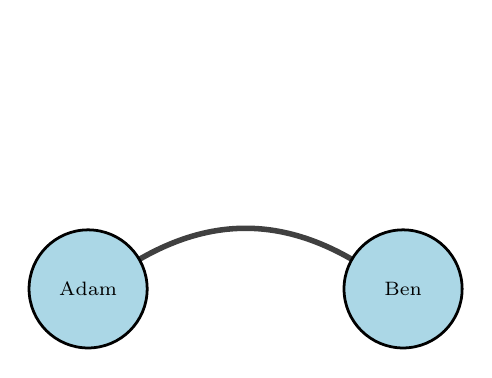
\begin{tikzpicture}
			\Vertex[label=Adam, y=-2, size=1.5]{A}
			\Vertex[label=Ben, x=4, y=-2, size=1.5]{B}
			\Vertex[Pseudo, x=4, y=1]{P}
			\Edge[bend=30,lw=2](A)(B)
		\end{tikzpicture}
	}
	\end{center}
\end{frame}

\begin{frame}
	\frametitle{Temporal networks}
	\begin{center}
	\resizebox{0.75\textwidth}{!}{
		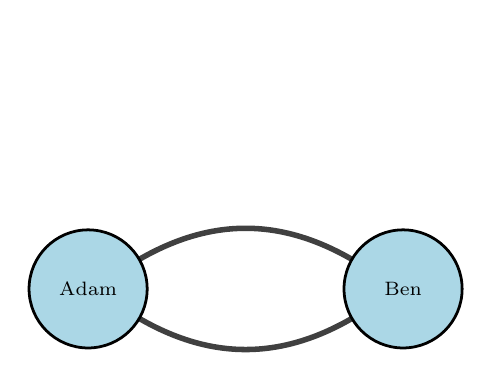
\begin{tikzpicture}
			\Vertex[label=Adam, y=-2, size=1.5]{A}
			\Vertex[label=Ben, x=4, y=-2, size=1.5]{B}
			\Vertex[Pseudo, x=4, y=1]{P}
			\Edge[bend=30,lw=2](A)(B)
			\Edge[bend=-30,lw=2](A)(B)
		\end{tikzpicture}
	}
	\end{center}
\end{frame}

\begin{frame}
	\frametitle{Temporal networks}
	\begin{center}
	\resizebox{0.75\textwidth}{!}{
		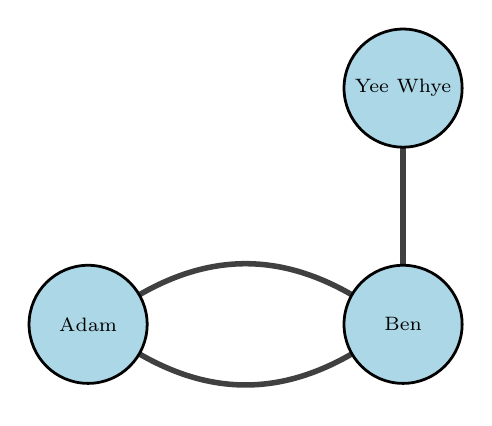
\begin{tikzpicture}
			\Vertex[label=Adam, y=-2, size=1.5]{A}
			\Vertex[label=Ben, x=4, y=-2, size=1.5]{B}
			\Vertex[label={Yee Whye}, x=4, y=1, size=1.5]{Y}
			\Edge[bend=30,lw=2](A)(B)
			\Edge[bend=-30,lw=2](A)(B)
			\Edge[lw=2](B)(Y)
		\end{tikzpicture}
	}
	\end{center}
\end{frame}

\begin{frame}
	\frametitle{Temporal networks}
	\begin{center}
	\resizebox{0.75\textwidth}{!}{
		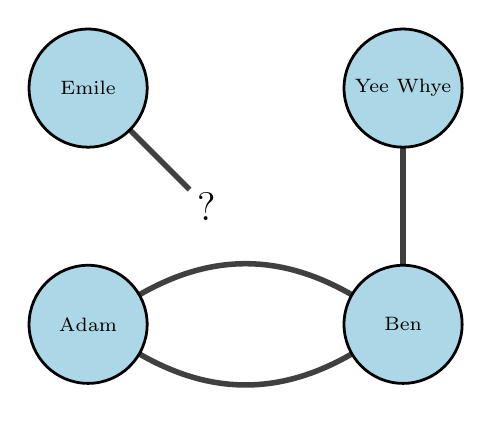
\begin{tikzpicture}
			\Vertex[label=Adam, y=-2, size=1.5]{A}
			\Vertex[label=Ben, x=4, y=-2, size=1.5]{B}
			\Vertex[label={Yee Whye}, x=4, y=1, size=1.5]{Y}
			\Vertex[label=Emile, y=1, size=1.5]{E}
			\Vertex[Pseudo,label={?}, x=1.5, y=-0.5, fontsize=\Large]{Ghost}
			\Edge[bend=30,lw=2](A)(B)
			\Edge[bend=-30,lw=2](A)(B)
			\Edge[lw=2](B)(Y)
			\Edge[lw=2](E)(Ghost)
		\end{tikzpicture}
	}
	\end{center}
\end{frame}

\begin{frame}
	\frametitle{Temporal networks}
	\begin{center}
	\resizebox{0.75\textwidth}{!}{
		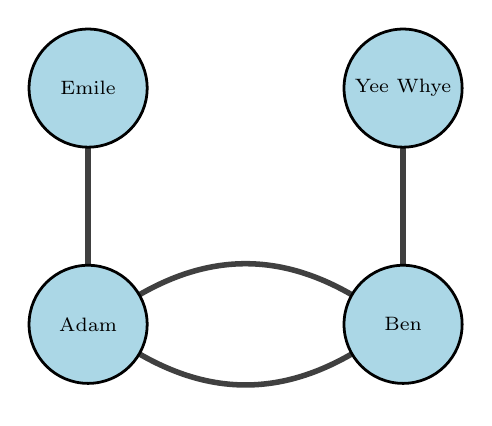
\begin{tikzpicture}
			\Vertex[label=Adam, y=-2, size=1.5]{A}
			\Vertex[label=Ben, x=4, y=-2, size=1.5]{B}
			\Vertex[label={Yee Whye}, x=4, y=1, size=1.5]{Y}
			\Vertex[label=Emile, y=1, size=1.5]{E}
			\Edge[bend=30,lw=2](A)(B)
			\Edge[bend=-30,lw=2](A)(B)
			\Edge[lw=2](B)(Y)
			\Edge[lw=2](E)(A)
		\end{tikzpicture}
	}
	\end{center}
\end{frame}

% \begin{frame}
% 	\frametitle{Temporal networks}
% 	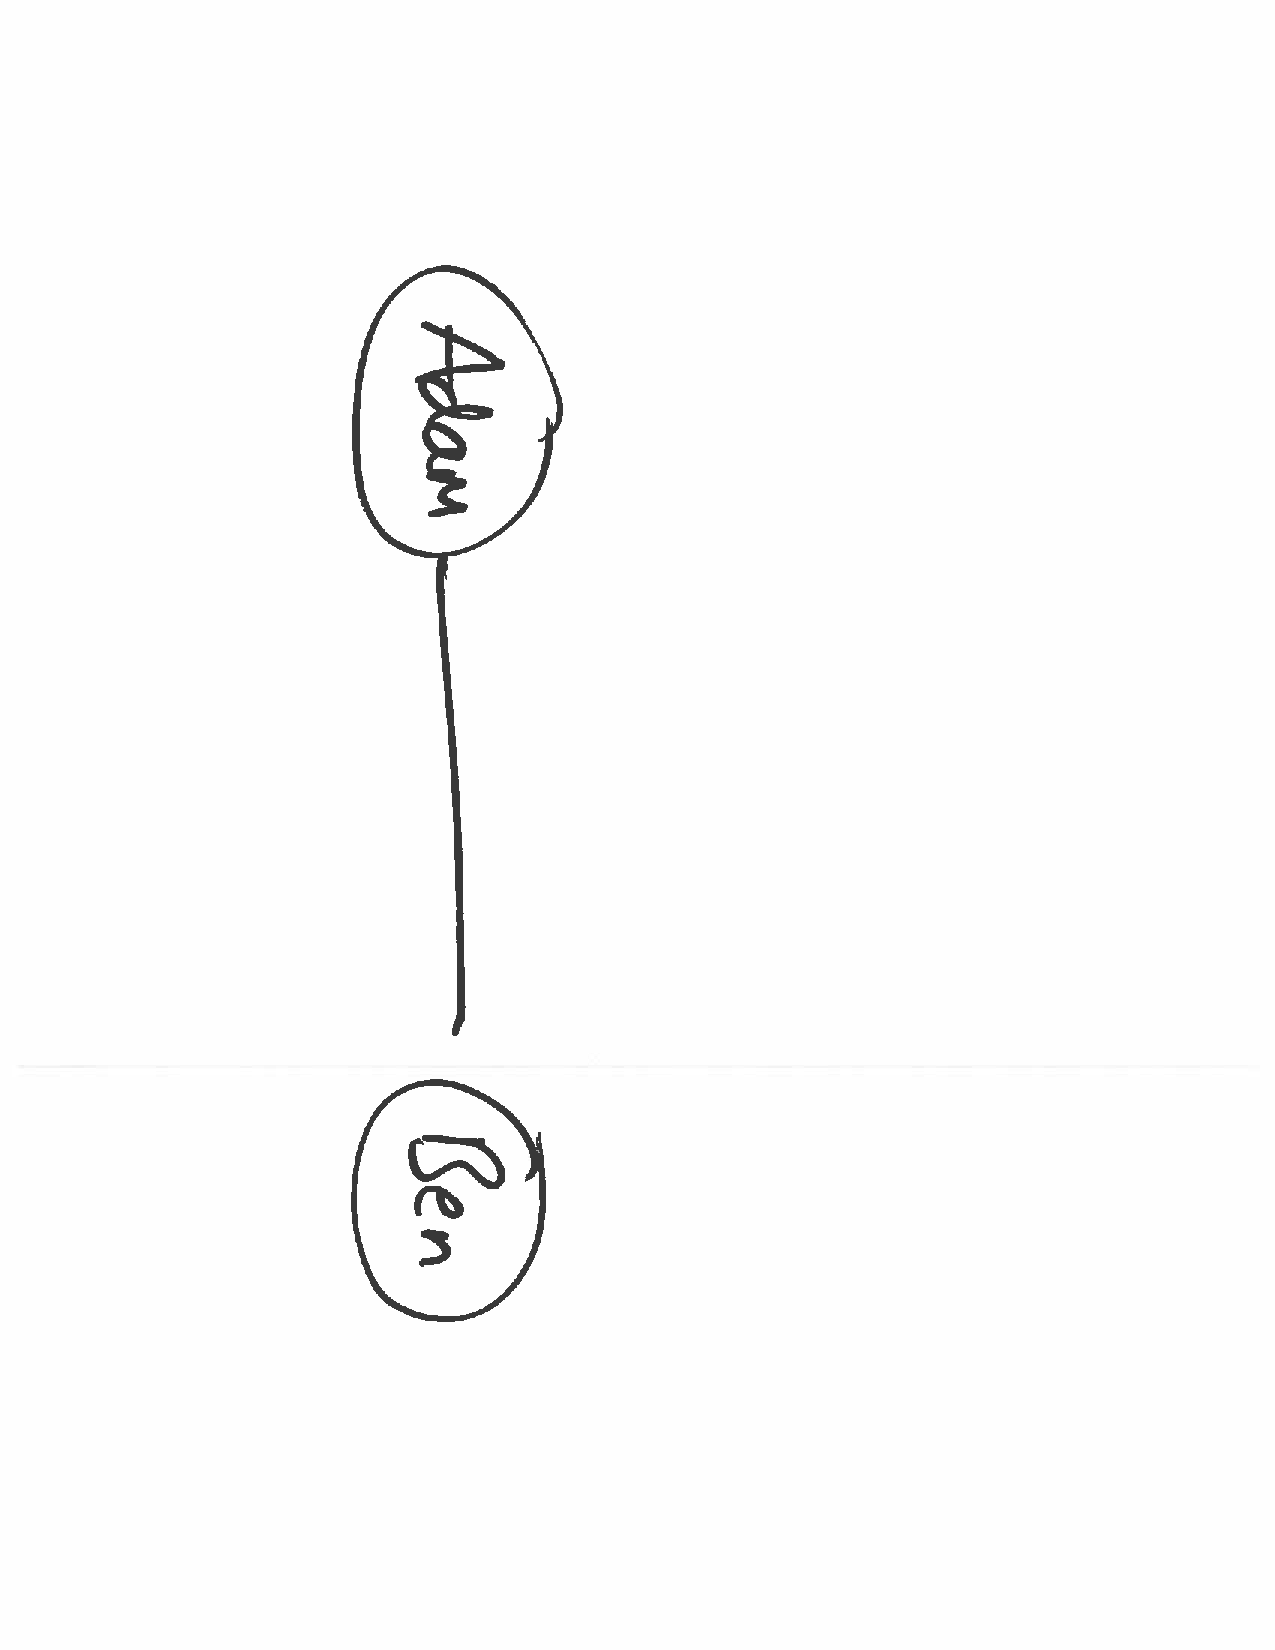
\includegraphics[angle=90,origin=c,scale=0.4]{fig/socialnet1}
% \end{frame}

% \begin{frame}
% 	\frametitle{Temporal networks}
% 	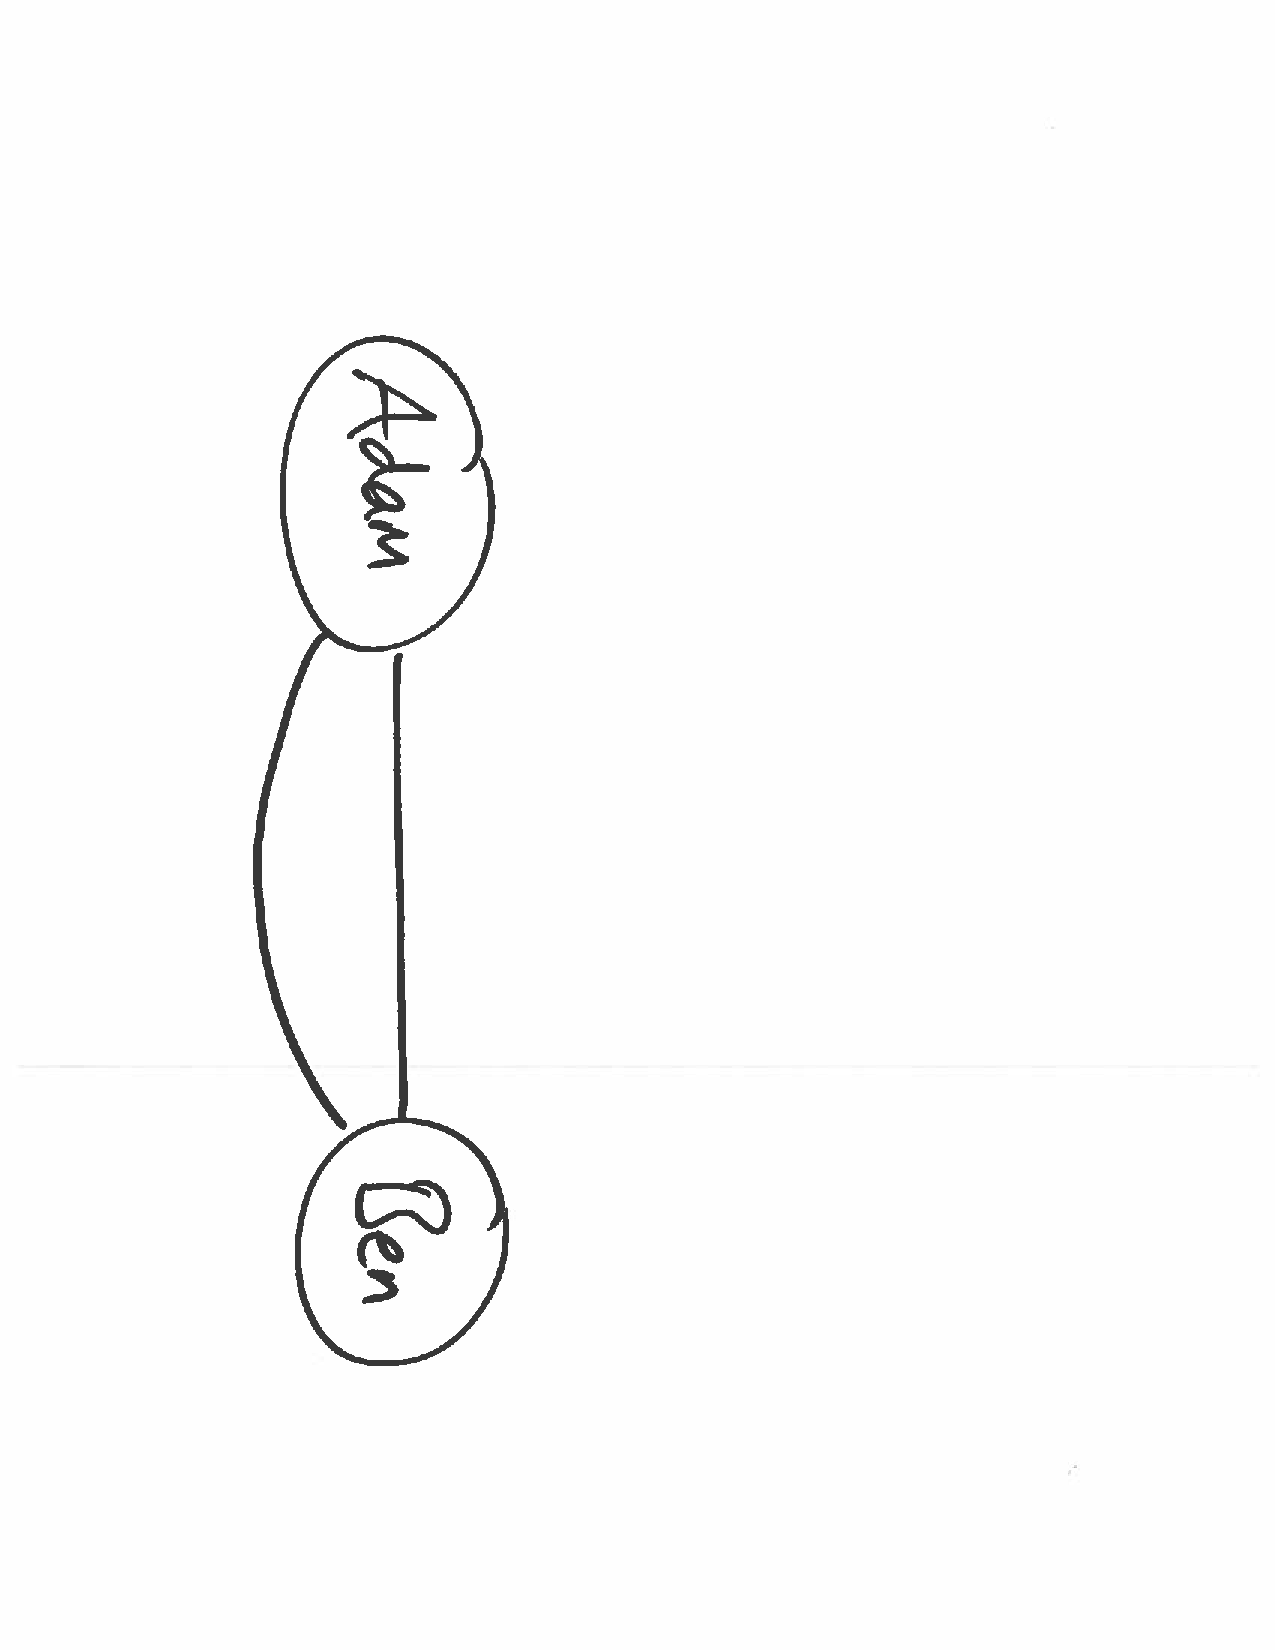
\includegraphics[angle=270,origin=c,scale=0.4]{fig/socialnet2}
% \end{frame}

% \begin{frame}
% 	\frametitle{Temporal networks}
% 	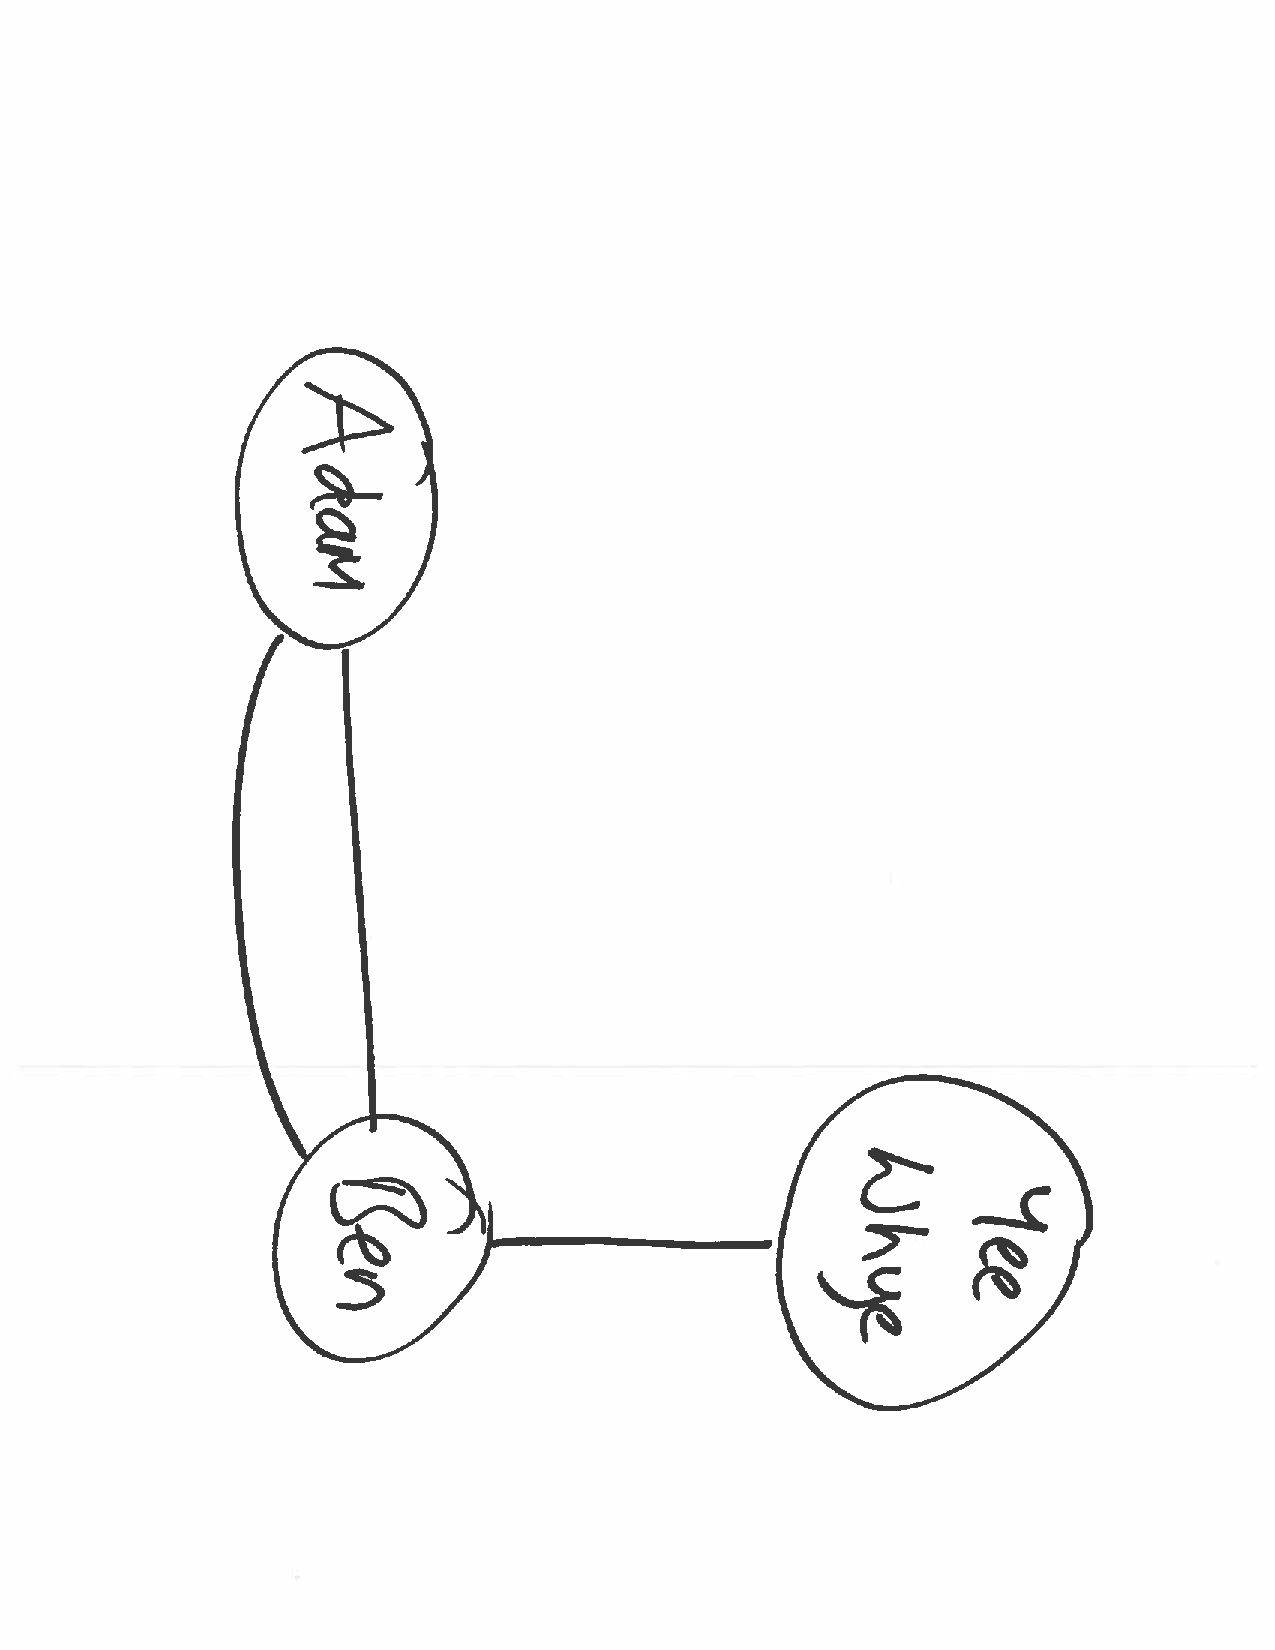
\includegraphics[angle=90,origin=c,scale=0.4]{fig/socialnet3}
% \end{frame}

% \begin{frame}
% 	\frametitle{Temporal networks}
% 	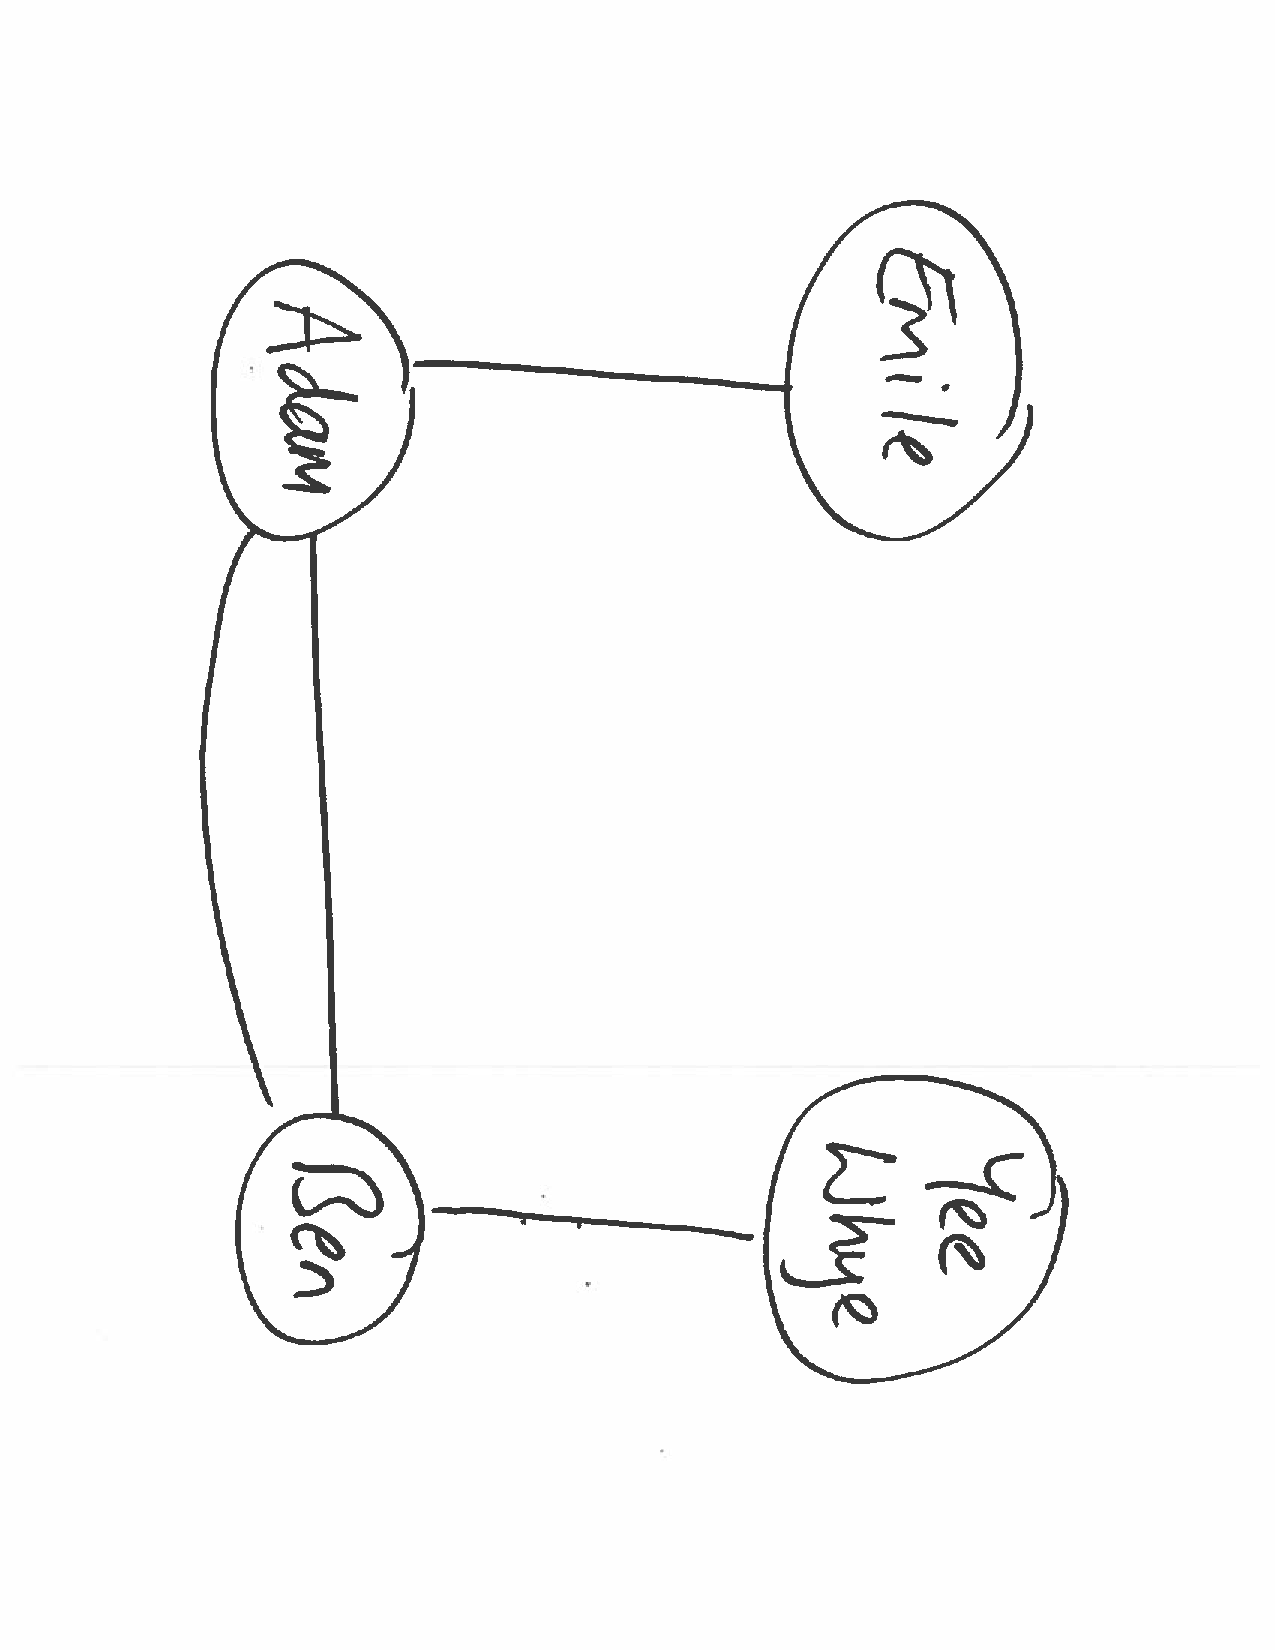
\includegraphics[angle=90,origin=c,scale=0.4]{fig/socialnet4}
% \end{frame}

% step function for edges and vertices graph
\pgfplotstableread{
1 1
2 1
3 2
4 2
5 3
6 3
7 3
8 3
}\datatable

\begin{frame}
	\frametitle{Edges and vertices}
	\begin{center}
	\only<1-4>{
	  \resizebox{0.65\textwidth}{!}{
		\begin{tikzpicture}
			\begin{axis}[
				axis lines = left,
				xlabel = {Number of edges},
				ylabel = {Vertex i.d.},
				xtick = {1,2,3,4},
				ytick = {1,2,3},
				xmin = 0,
				xmax = 4.5,
				ymax = 4,
				ymin = 0,
				style = thick
			]
			% \addplot+[ultra thick, const plot, no marks,color=darkblue] table [x index=0, y index=1]{\datatable};
			% \draw (axis cs:1,0.5) -- (axis cs:2,0.5);
			\only<1-4>{\fill[color=blueClj] (axis cs:.5,1) circle (5pt);}
			\only<1-4>{\fill[color=blueClj] (axis cs:1,1) circle (5pt);}
			\only<2-4>{\fill[color=orangeClj] (axis cs:1.5,2) circle (5pt);}
			\only<2-4>{\fill[color=blueClj] (axis cs:2,1) circle (5pt);}
			\only<3-4>{\fill[color=darkgreenClj] (axis cs:2.5,3) circle (5pt);}
			\only<3-4>{\fill[color=blueClj] (axis cs:3,1) circle (5pt);}
			\only<4>{\fill[color=orangeClj] (axis cs:3.5,2) circle (5pt);}
			\only<4>{\fill[color=darkgreenClj] (axis cs:4,3) circle (5pt);}
			\end{axis}
		\end{tikzpicture}
	  }
		\begin{tikzpicture}
			\only<1-4>{
				\Vertex[color=blueClj,label=1,x=0,y=0]{v1}
				\Vertex[Pseudo,x=2,y=0]{pv} % just to get the spacing right across slides
				\Edge[loopposition=180,lw=2](v1)(v1)
			}
			\only<2-4>{
				\Vertex[color=orangeClj,label=2,x=2,y=0]{v2}
				\Edge[lw=2](v2)(v1)
			}
			\only<3-4>{
				\Vertex[color=darkgreenClj,label=3,x=1,y=1]{v3}
				\Edge[lw=2](v3)(v1)
			}
			\only<4>{
				\Edge[lw=2](v3)(v2)
			}
		\end{tikzpicture}
	}
	\end{center}
\end{frame}

% \begin{frame}
% 	\frametitle{Edges and vertices}
% 	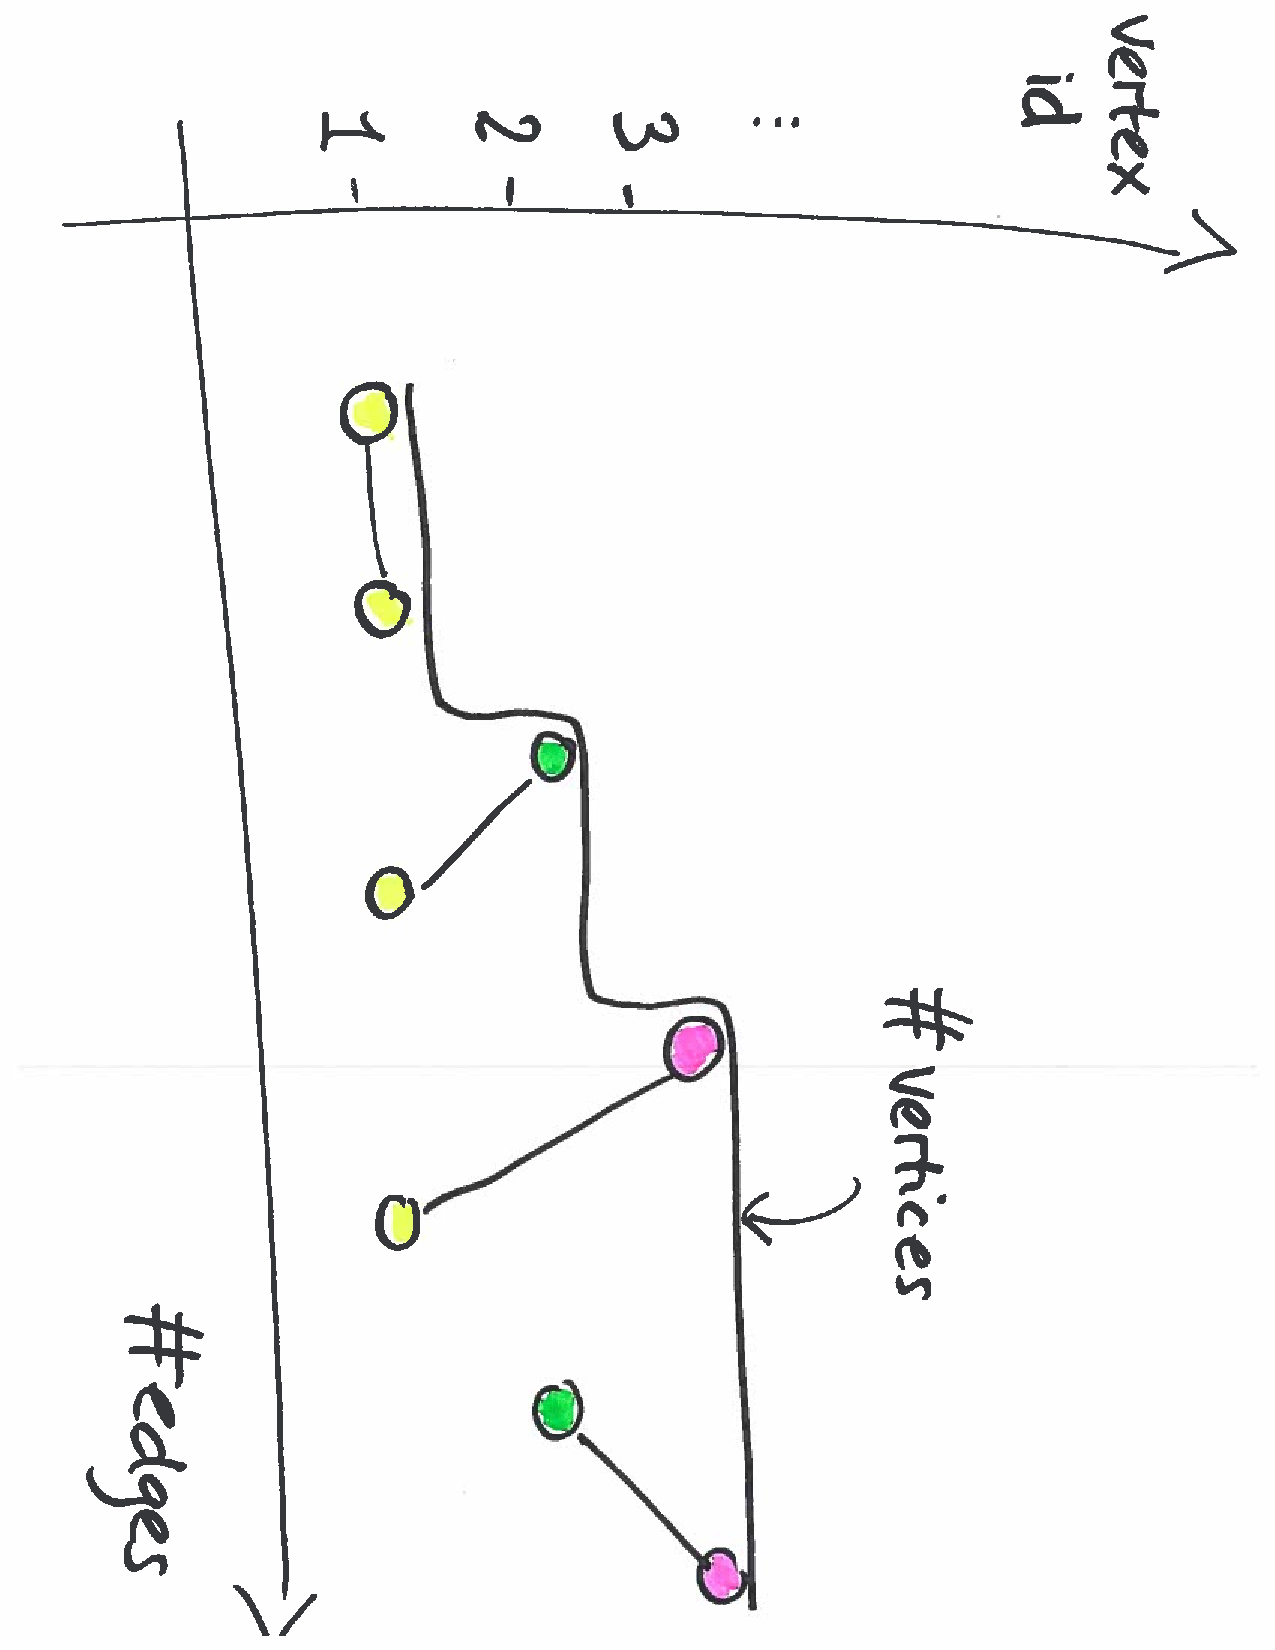
\includegraphics[angle=90,origin=c,scale=0.4]{fig/edgevertex}
% \end{frame}


% \begin{frame}
% 	\frametitle{Sparsity}
% 	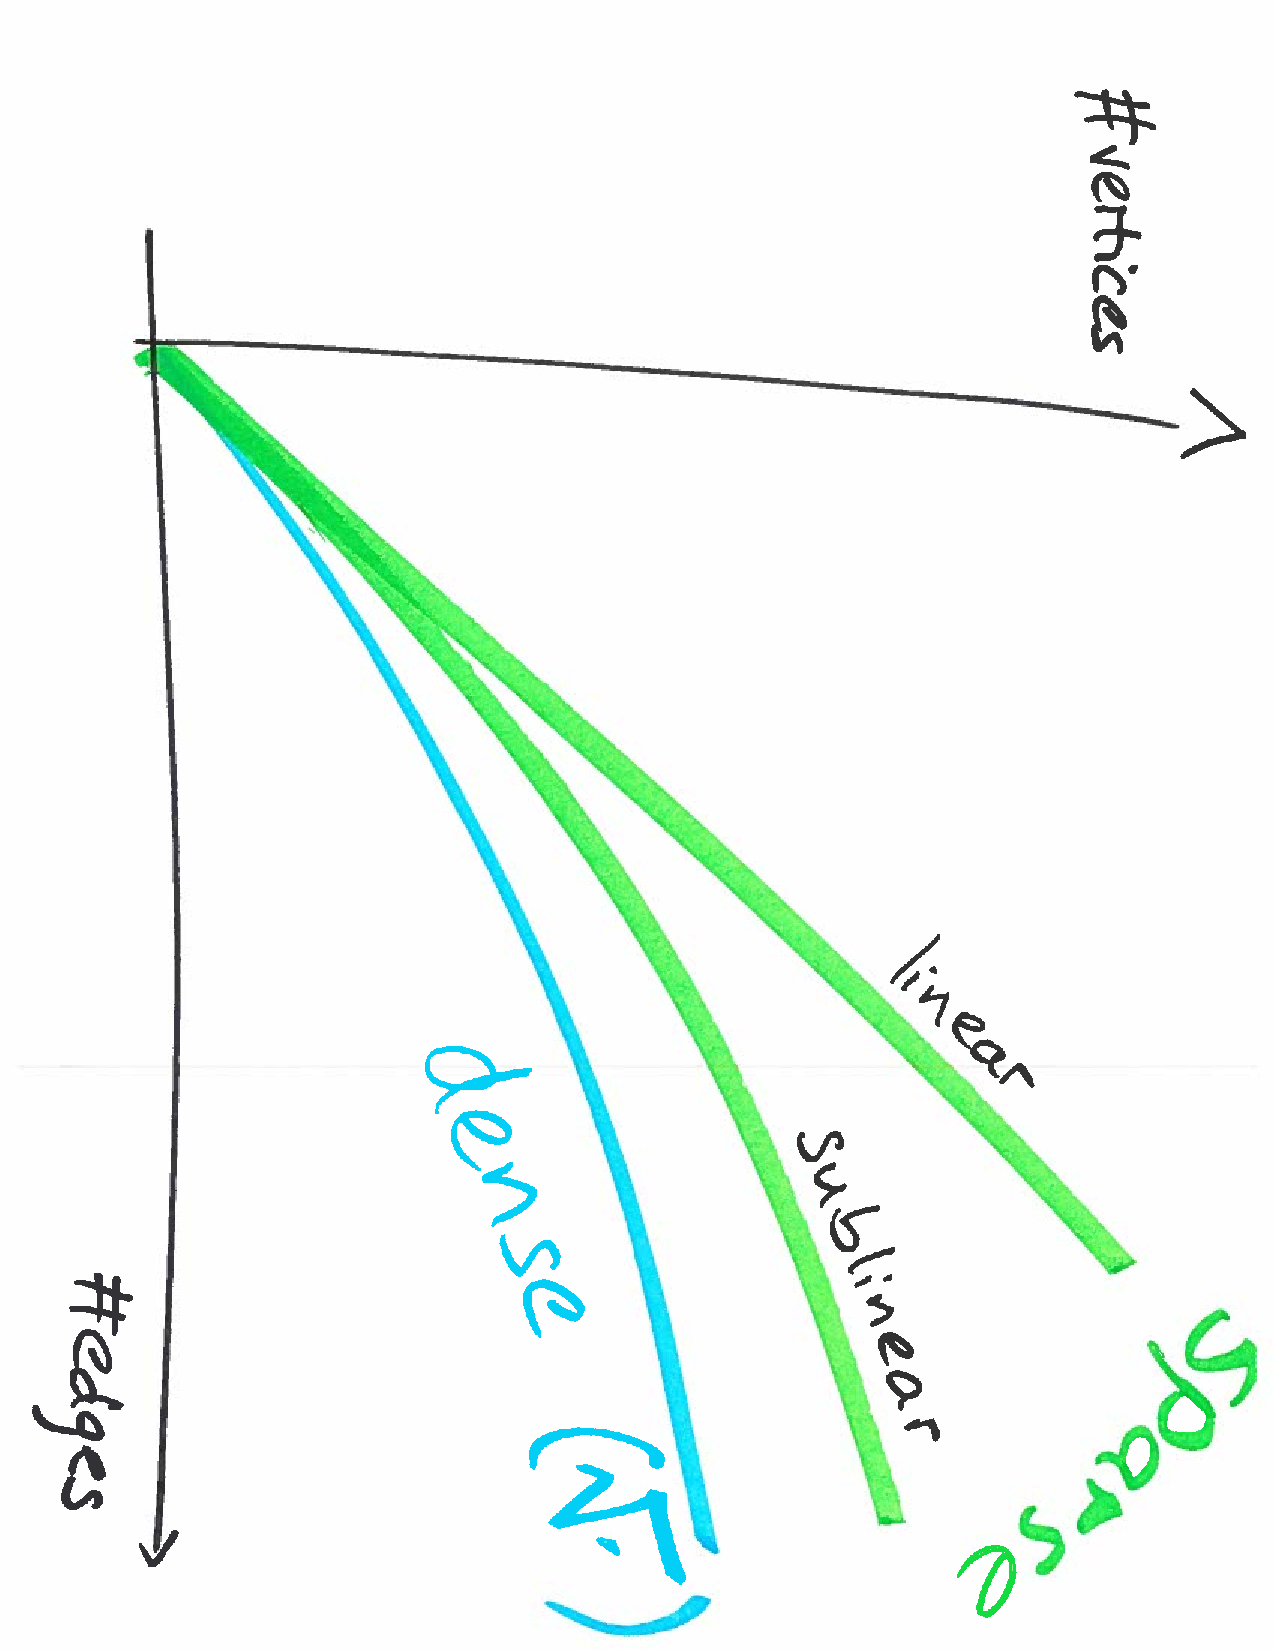
\includegraphics[angle=90,origin=c,scale=0.4]{fig/sparsity}
% \end{frame}

\begin{frame}
	\frametitle{Sparsity}
	\begin{center}
		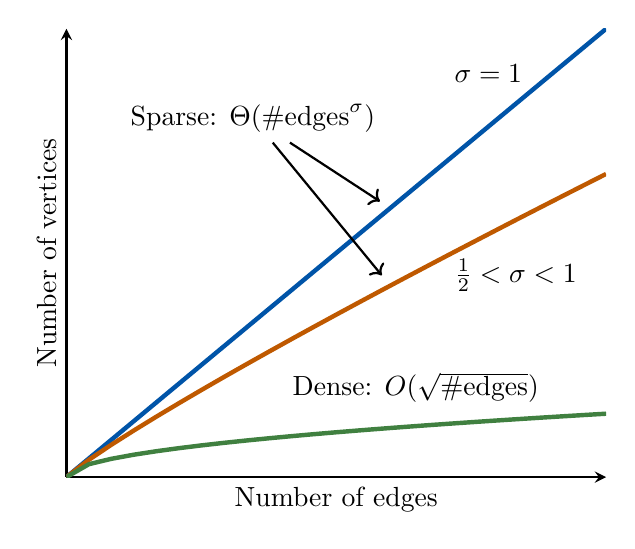
\begin{tikzpicture}
			\begin{axis}[
				axis lines = left,
				xlabel = {Number of edges},
				ylabel = {Number of vertices},
				ticks = none,
				style = thick
			]
				\addplot[color=blueClj,domain=0:50,style=ultra thick]{x};
				\addplot[color=orangeClj,domain=0:50,style=ultra thick]{x^(0.9)};
				\addplot[color=darkgreenClj,domain=0:50,style=ultra thick]{x^(0.5)};
				\node[anchor=west] (sparse) at (axis cs:5,40){\normalsize Sparse: $\Theta(\text{\#edges}^{\sigma})$};
				\node (l1) at (axis cs:30,30){};
				\node (l2) at (axis cs:30,21.35){};
				\draw[->](sparse)--(l1);
				\draw[->](sparse)--(l2);
				\node[anchor=west] (dense) at (axis cs:20,10){\normalsize Dense: $O(\sqrt{\text{\#edges}})$};
				\node[anchor=west] (sig1) at (axis cs:35,45){$\sigma=1$};
				\node[anchor=west] (sig2) at (axis cs:35,22.5){$\frac{1}{2}<\sigma<1$};
			\end{axis}
		\end{tikzpicture}
	\end{center}
\end{frame}

% \begin{frame}
% 	\frametitle{Power law degree distribution}
% 	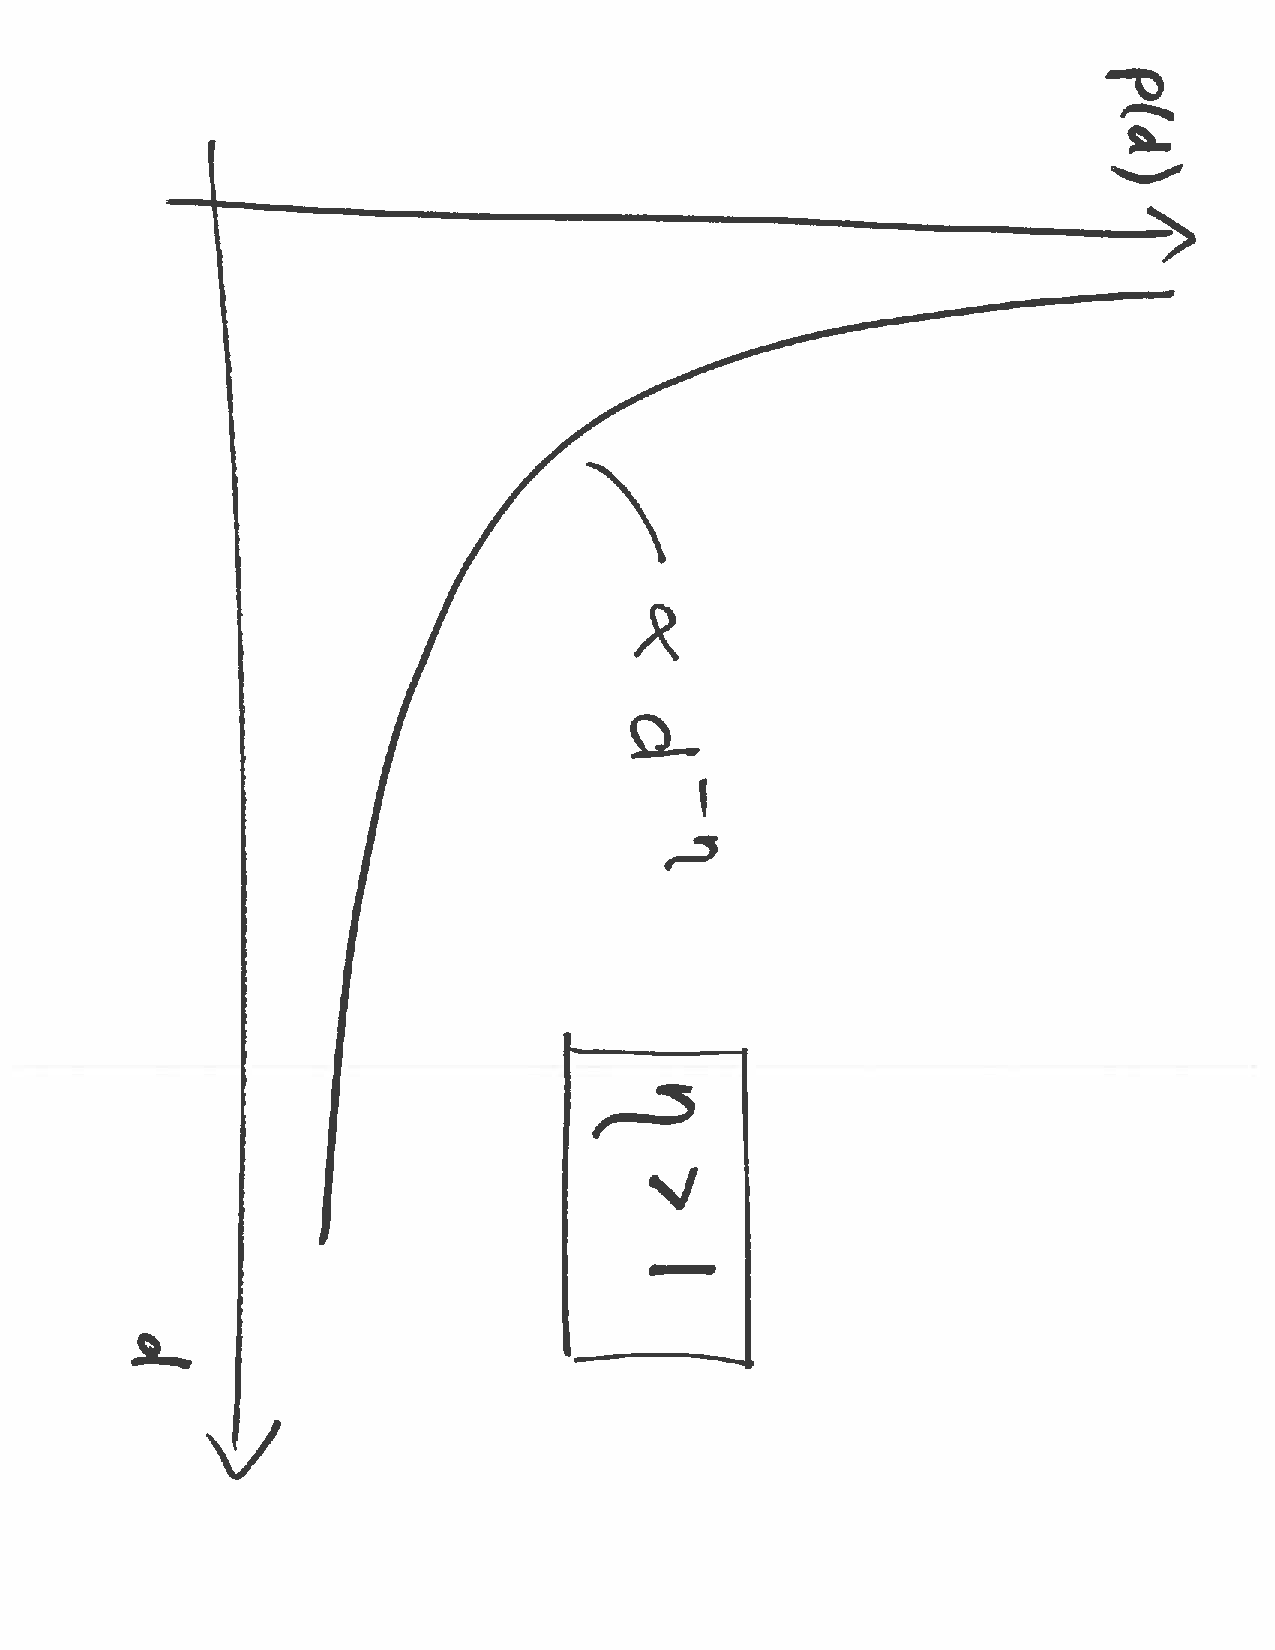
\includegraphics[angle=90,origin=c,scale=0.37]{fig/powerlaw}
% \end{frame}

\begin{frame}
	\frametitle{Power law degree distribution}
	\begin{center}
		$p(d) \propto d^{-\eta}$, for $\eta > 1$
		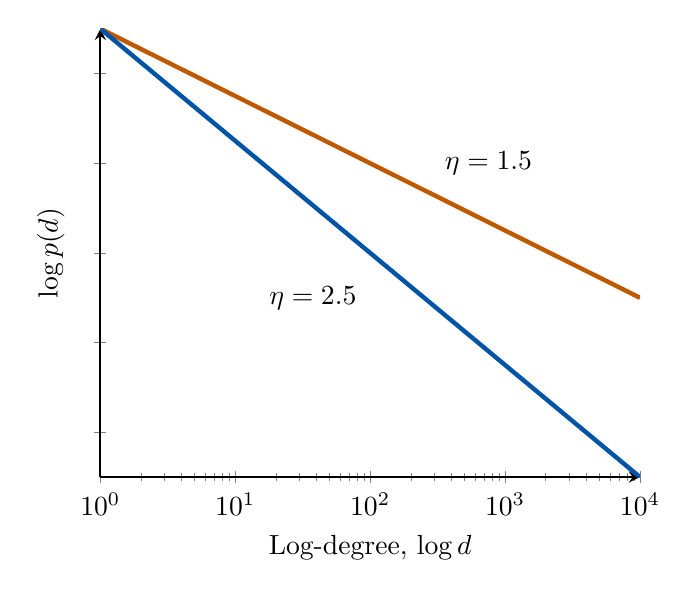
\begin{tikzpicture}
			\begin{axis}[
				ymode = log,
				xmode = log,
				axis lines = left,
				xlabel = {Log-degree, $\log d$},
				ylabel = {$\log p(d)$},
				style = thick,
				yticklabels = {,,}
				% xticklabels = {,,}
				% ymajorticks = false,
				% xmajorticks = false
			]
				\addplot[color=orangeClj,domain=1:10000,style=ultra thick]{x^(-1.5)};
				\addplot[color=blueClj,domain=1:10000,style=ultra thick]{x^(-2.5)};
				\node[anchor=west] (pl1) at (axis cs:300,0.001){$\eta=1.5$};
				\node[anchor=west] (pl2) at (axis cs:15,0.000001){$\eta=2.5$};
			\end{axis}
		\end{tikzpicture}
	\end{center}
\end{frame}

\begin{frame}
	\frametitle{Sparsity and power law}
	\begin{align*}
	\textbf{Sublinear } \text{sparsity} & \quad \iff \quad  \eta \in (1,2) \\
	\textbf{Linear } \text{sparsity} & \quad \iff \quad \eta > 2
	\end{align*}
\end{frame}

\begin{frame}
	\frametitle{Empirical study}
	\begin{table}[b]
		% \vspace*{-\baselineskip}
		\label{tab:datasets}
		\begin{center}
			\begin{tabular}{lll}
				SNAP dataset \cite{snapnets} & \# of vertices   & \# of edges    \\
				\hline
				Ask Ubuntu    & 159,316   & 964,437    \\
				UCI social network   & 1,899     & 20,296     \\
				\vdots & \vdots & \vdots
			\end{tabular}
		\end{center}
	\end{table}
	
\end{frame}

\begin{frame}
	\frametitle{Ask Ubuntu}
	\begin{figure}[h]
		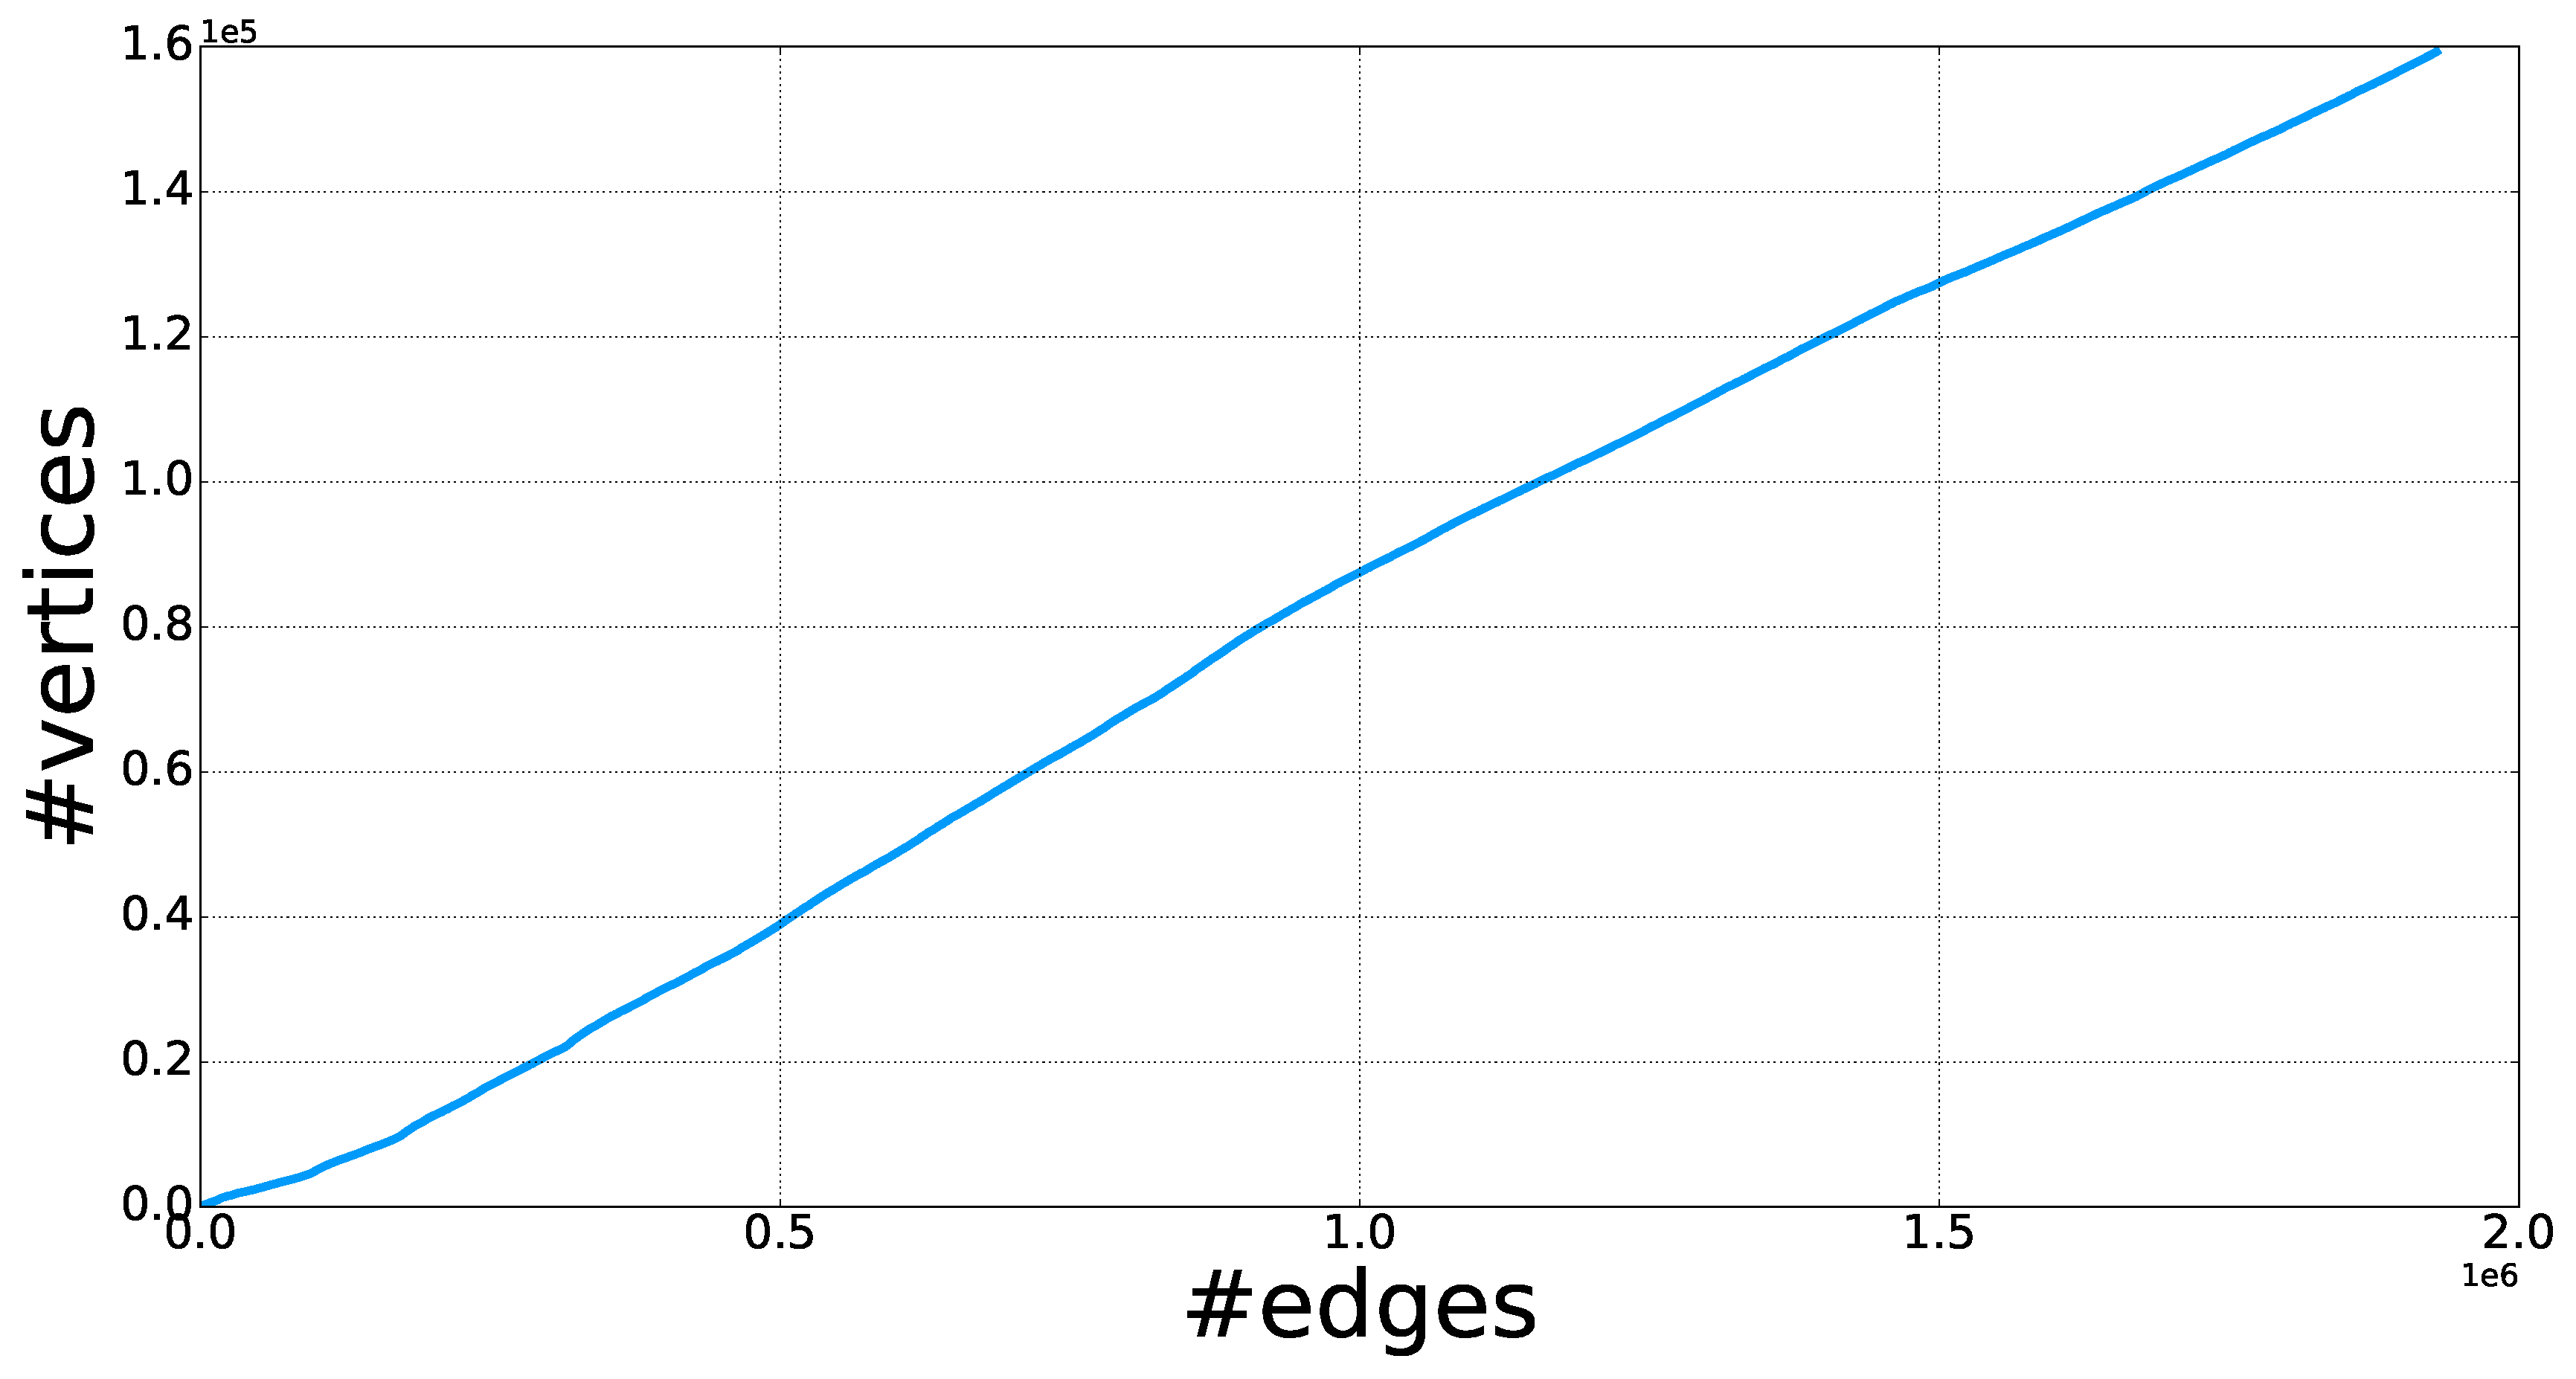
\includegraphics[width=1.0\textwidth]{fig/n_askubuntu_arrival.pdf}
	\end{figure}
	%$\hat{\sigma}=-0.0990787$
	%$\hat{\sigma} = -0.099$
\end{frame}

\begin{frame}
	\frametitle{UCI social network}
	\begin{figure}[h]
		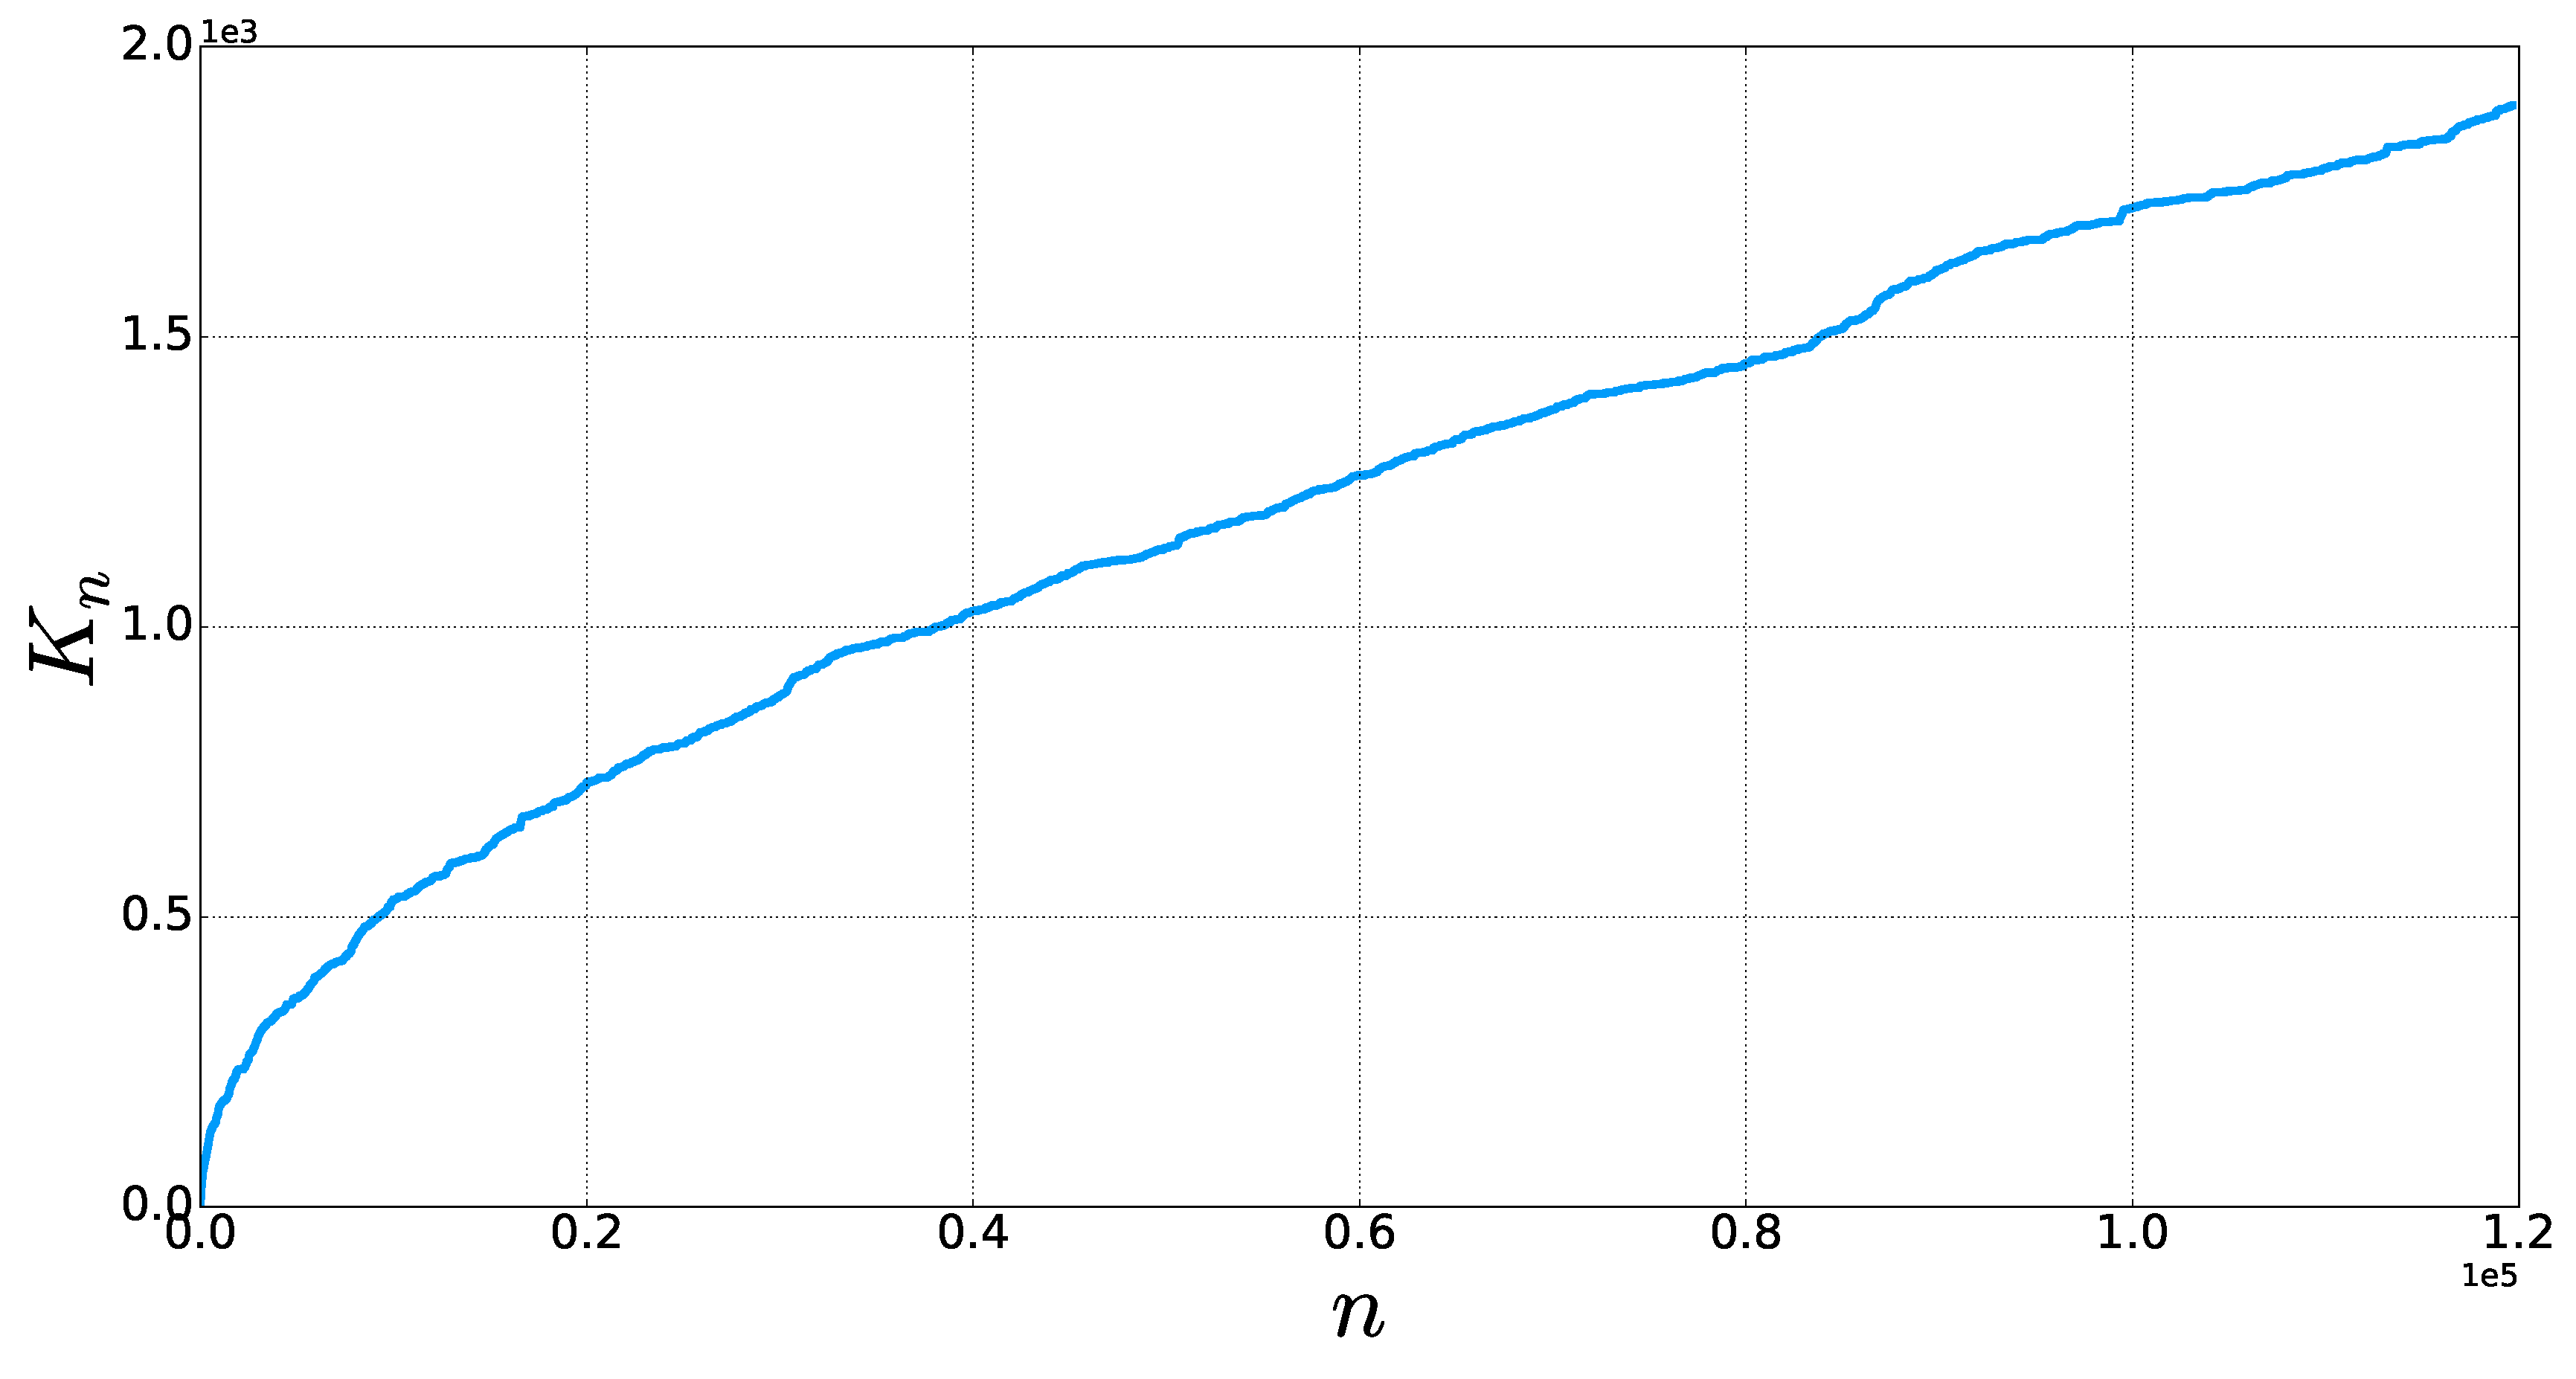
\includegraphics[width=1.0\textwidth]{fig/n_CollegeMsg_arrival.pdf}
	\end{figure}
	% $\sigma=0.95228934$
	% $\hat{\sigma} = 0.952$
\end{frame}

%\begin{frame}
%	\frametitle{Ask Ubuntu degree distribution}
%	\begin{figure}[h]
%		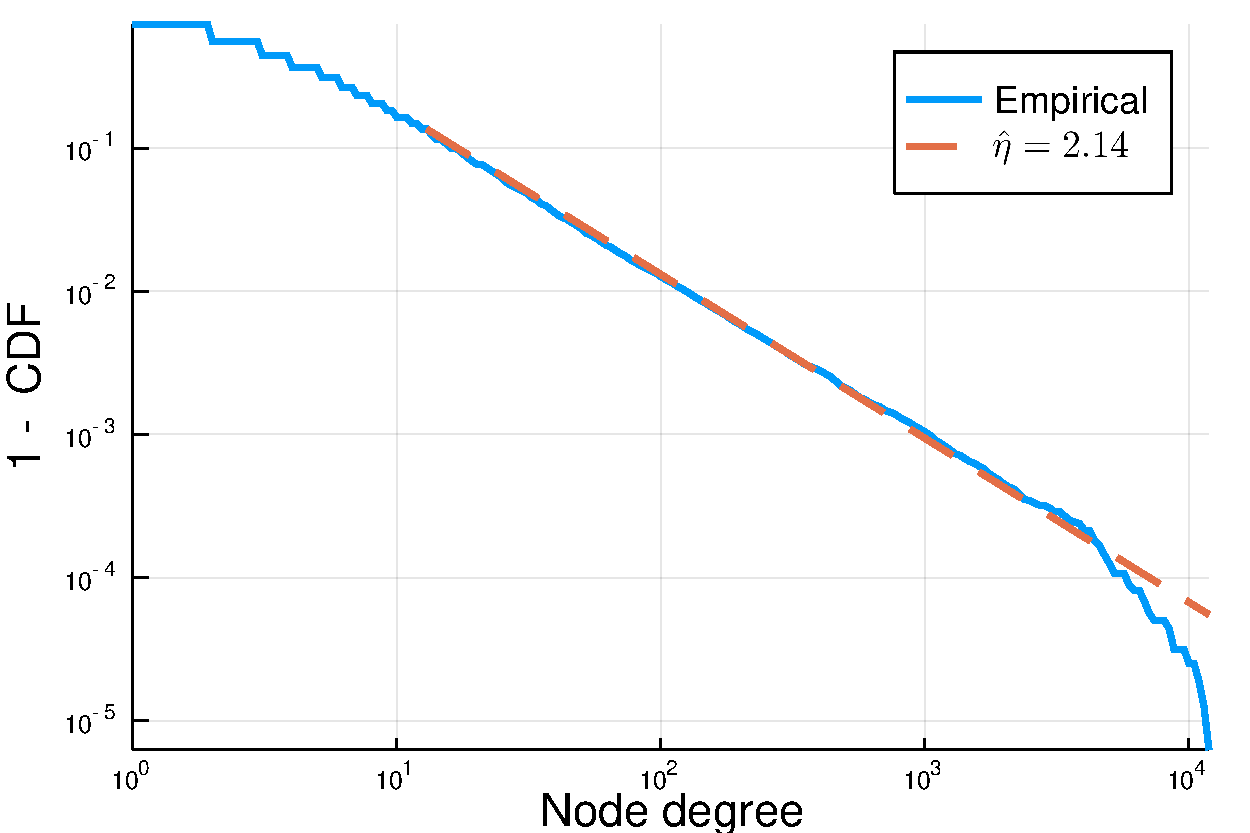
\includegraphics[width=0.8\textwidth]{fig/nodes_degre_power_law_askubuntu.pdf}
%	\end{figure}
%	
%	$\hat{\eta} = 2.14$ estimated using technique of \cite{clauset}
%	
%\end{frame}


\begin{frame}
	\frametitle{Models}
	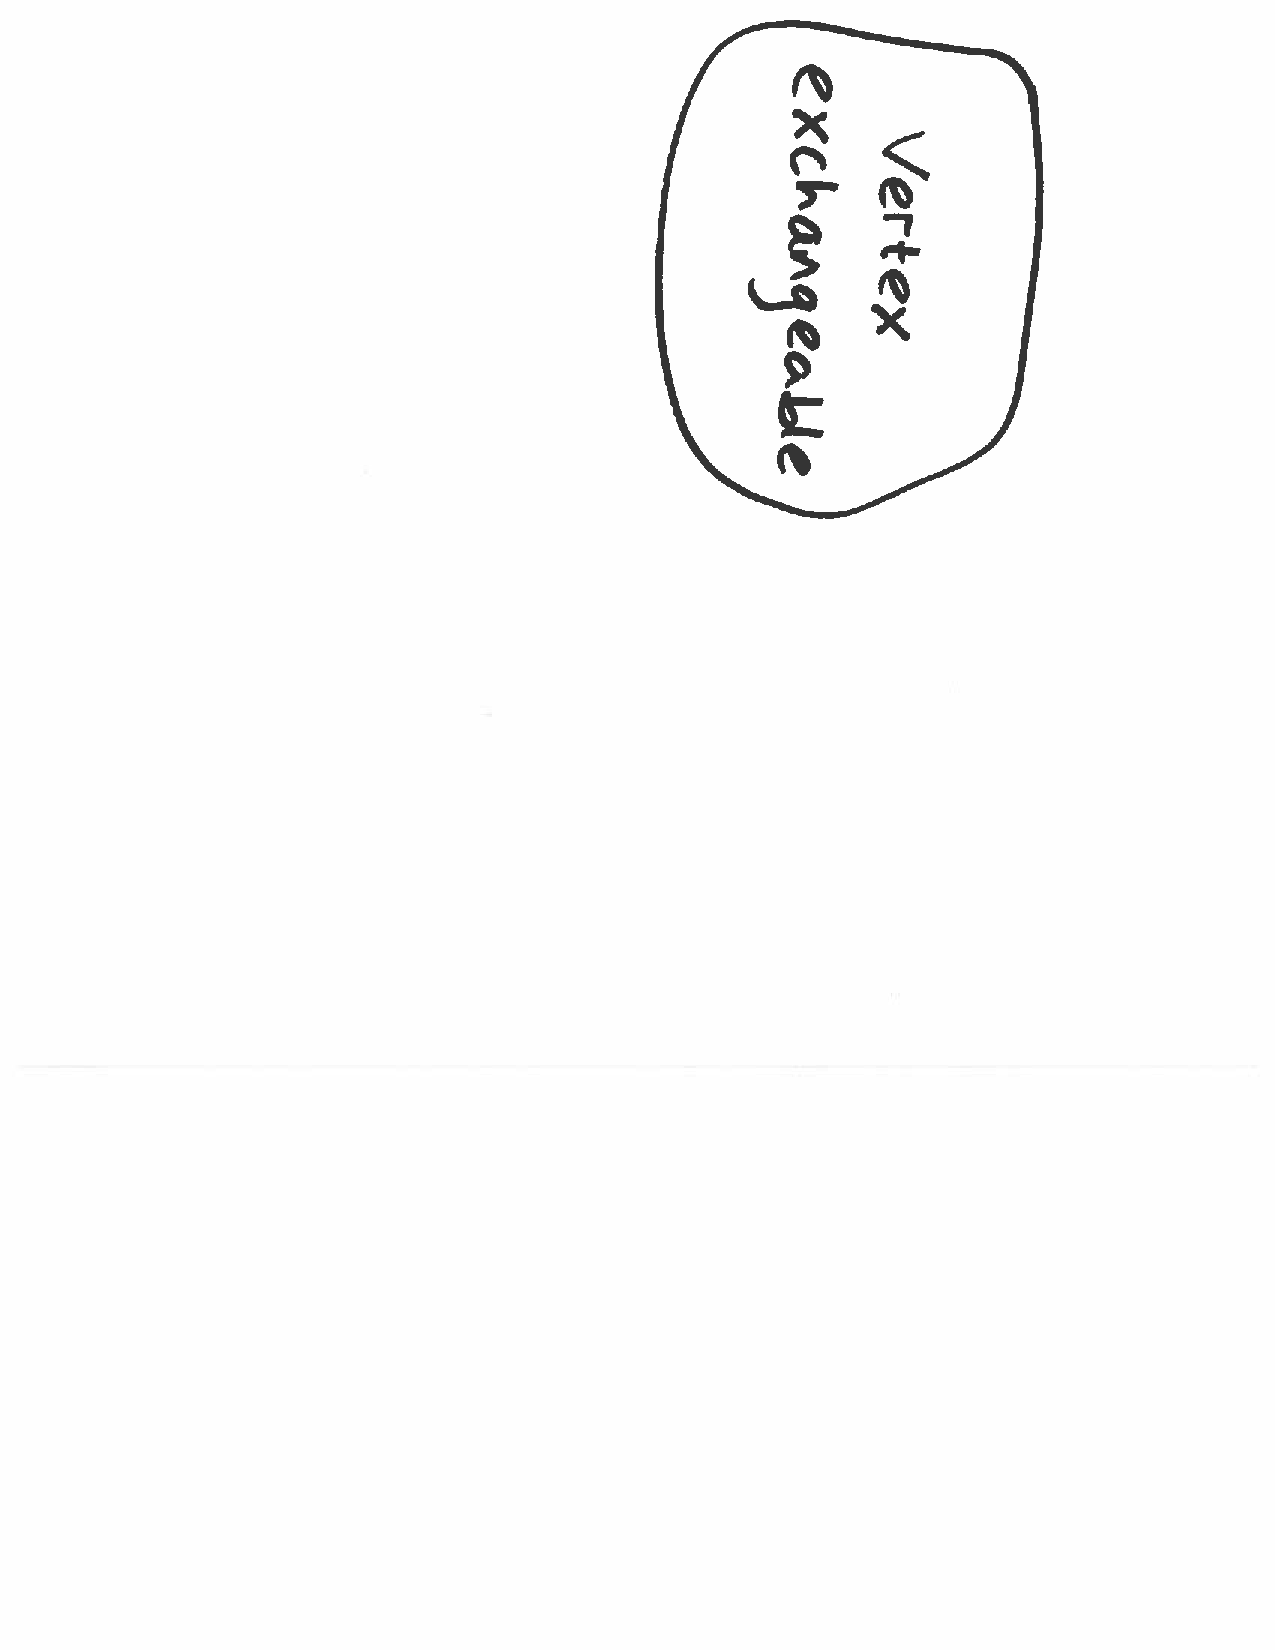
\includegraphics[angle=90,origin=c,scale=0.4]{fig/models1}
\end{frame}

\begin{frame}
	\frametitle{Models}
	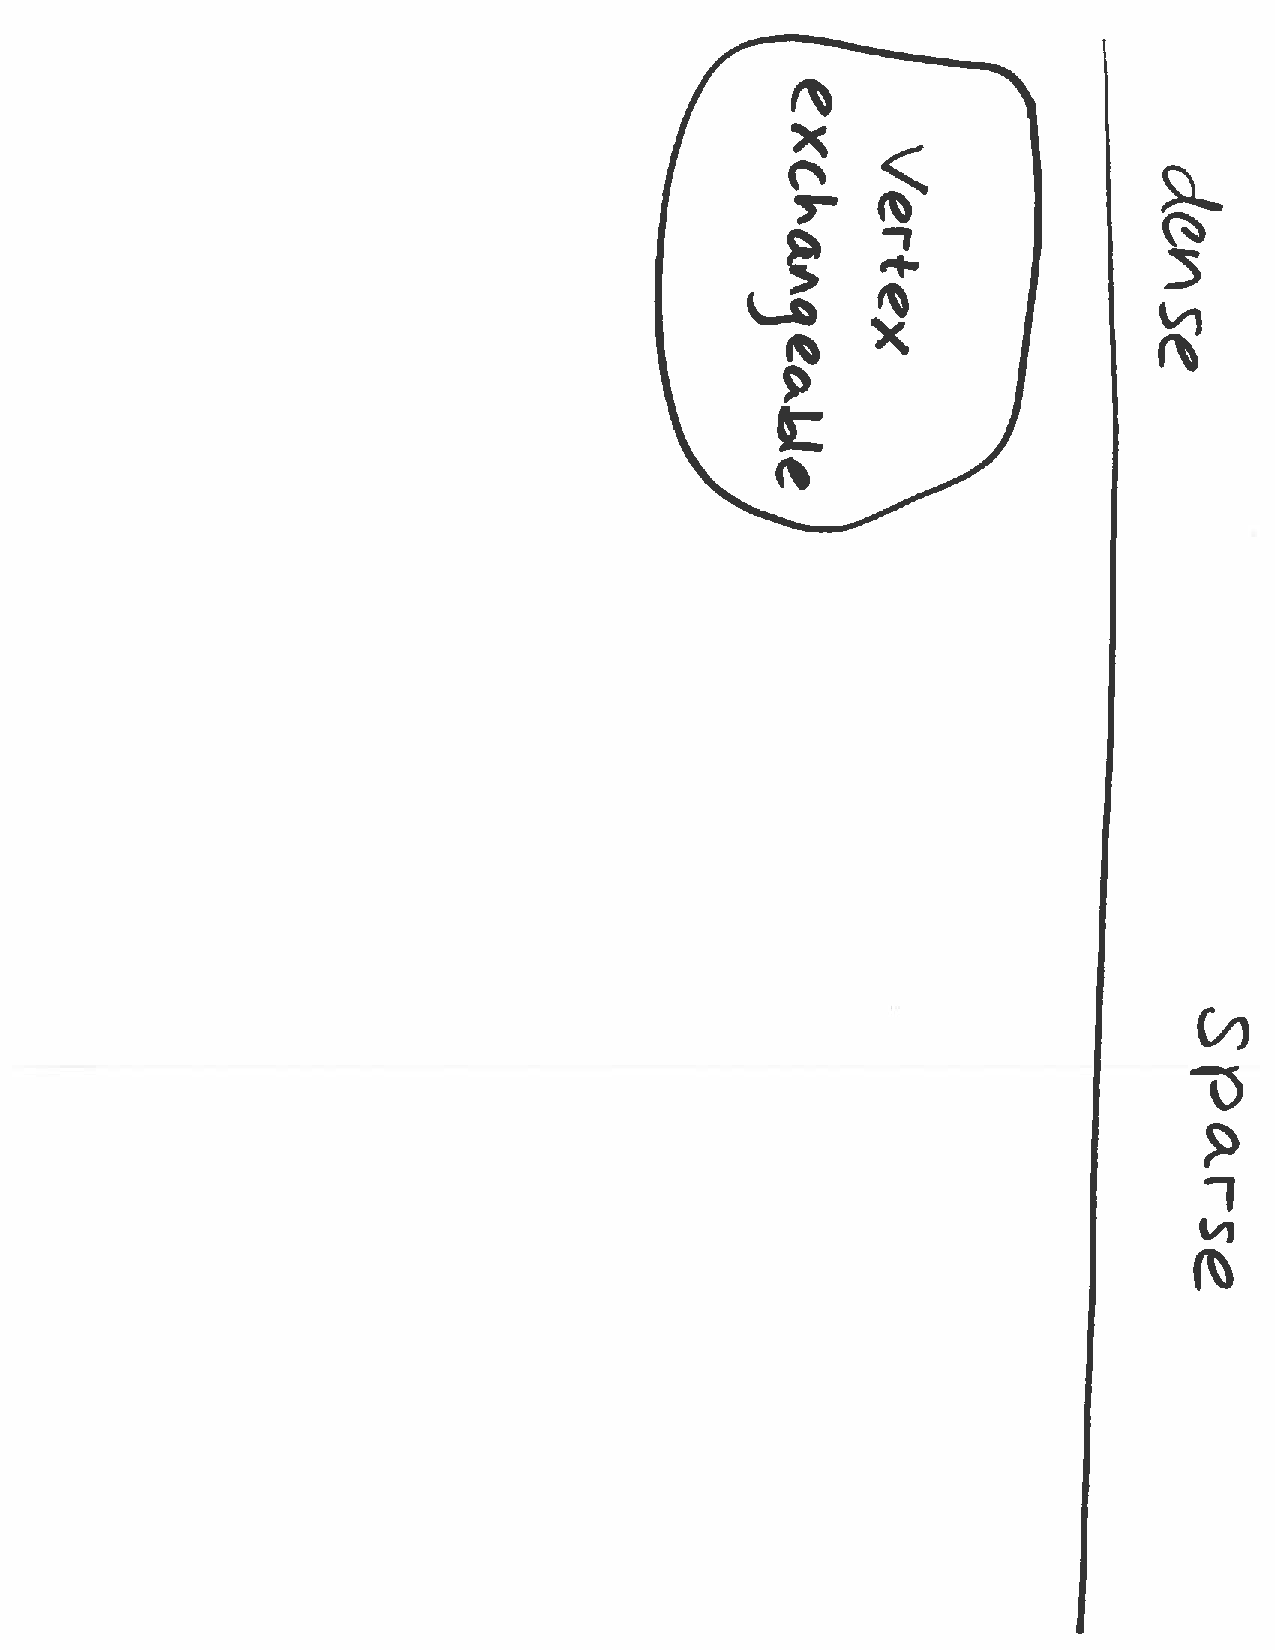
\includegraphics[angle=90,origin=c,scale=0.4]{fig/models2}
\end{frame}

\begin{frame}
	\frametitle{Models}
	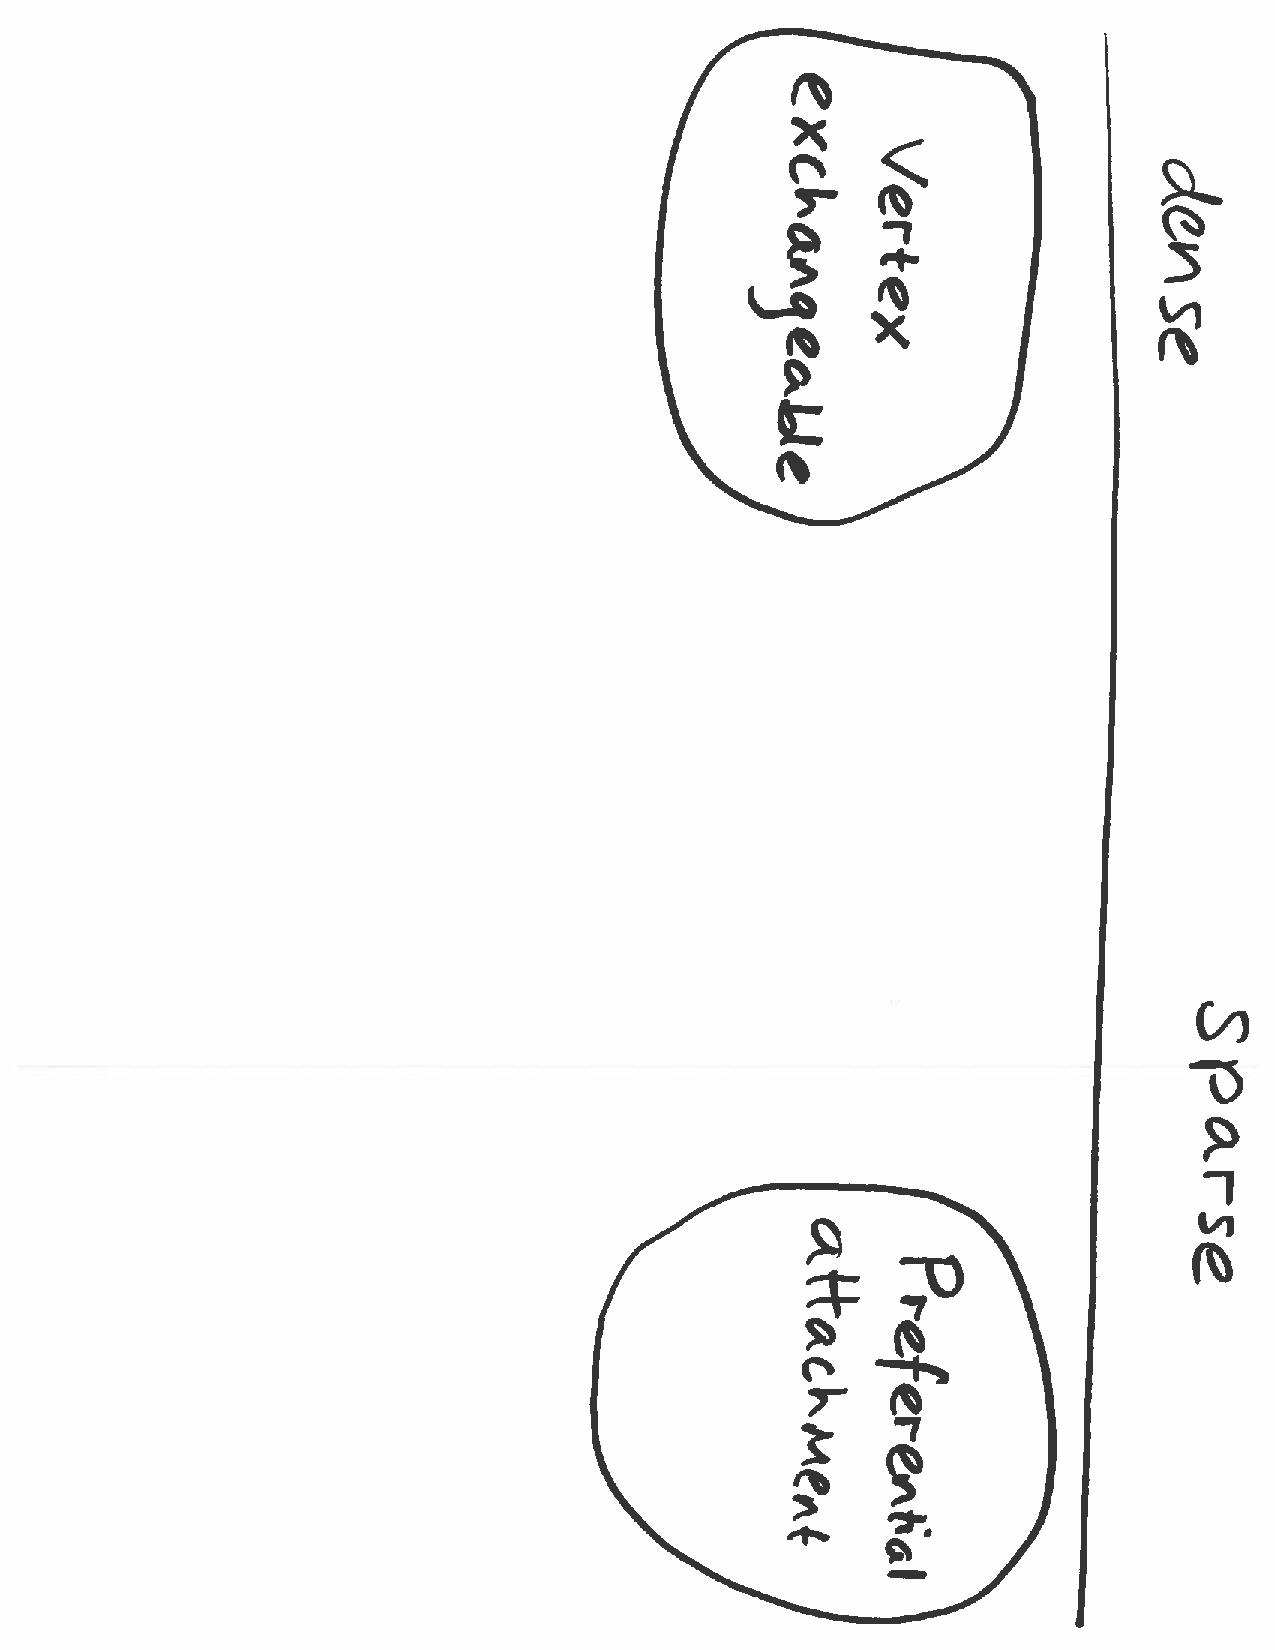
\includegraphics[angle=90,origin=c,scale=0.4]{fig/models3}
\end{frame}

\begin{frame}
	\frametitle{Models}
	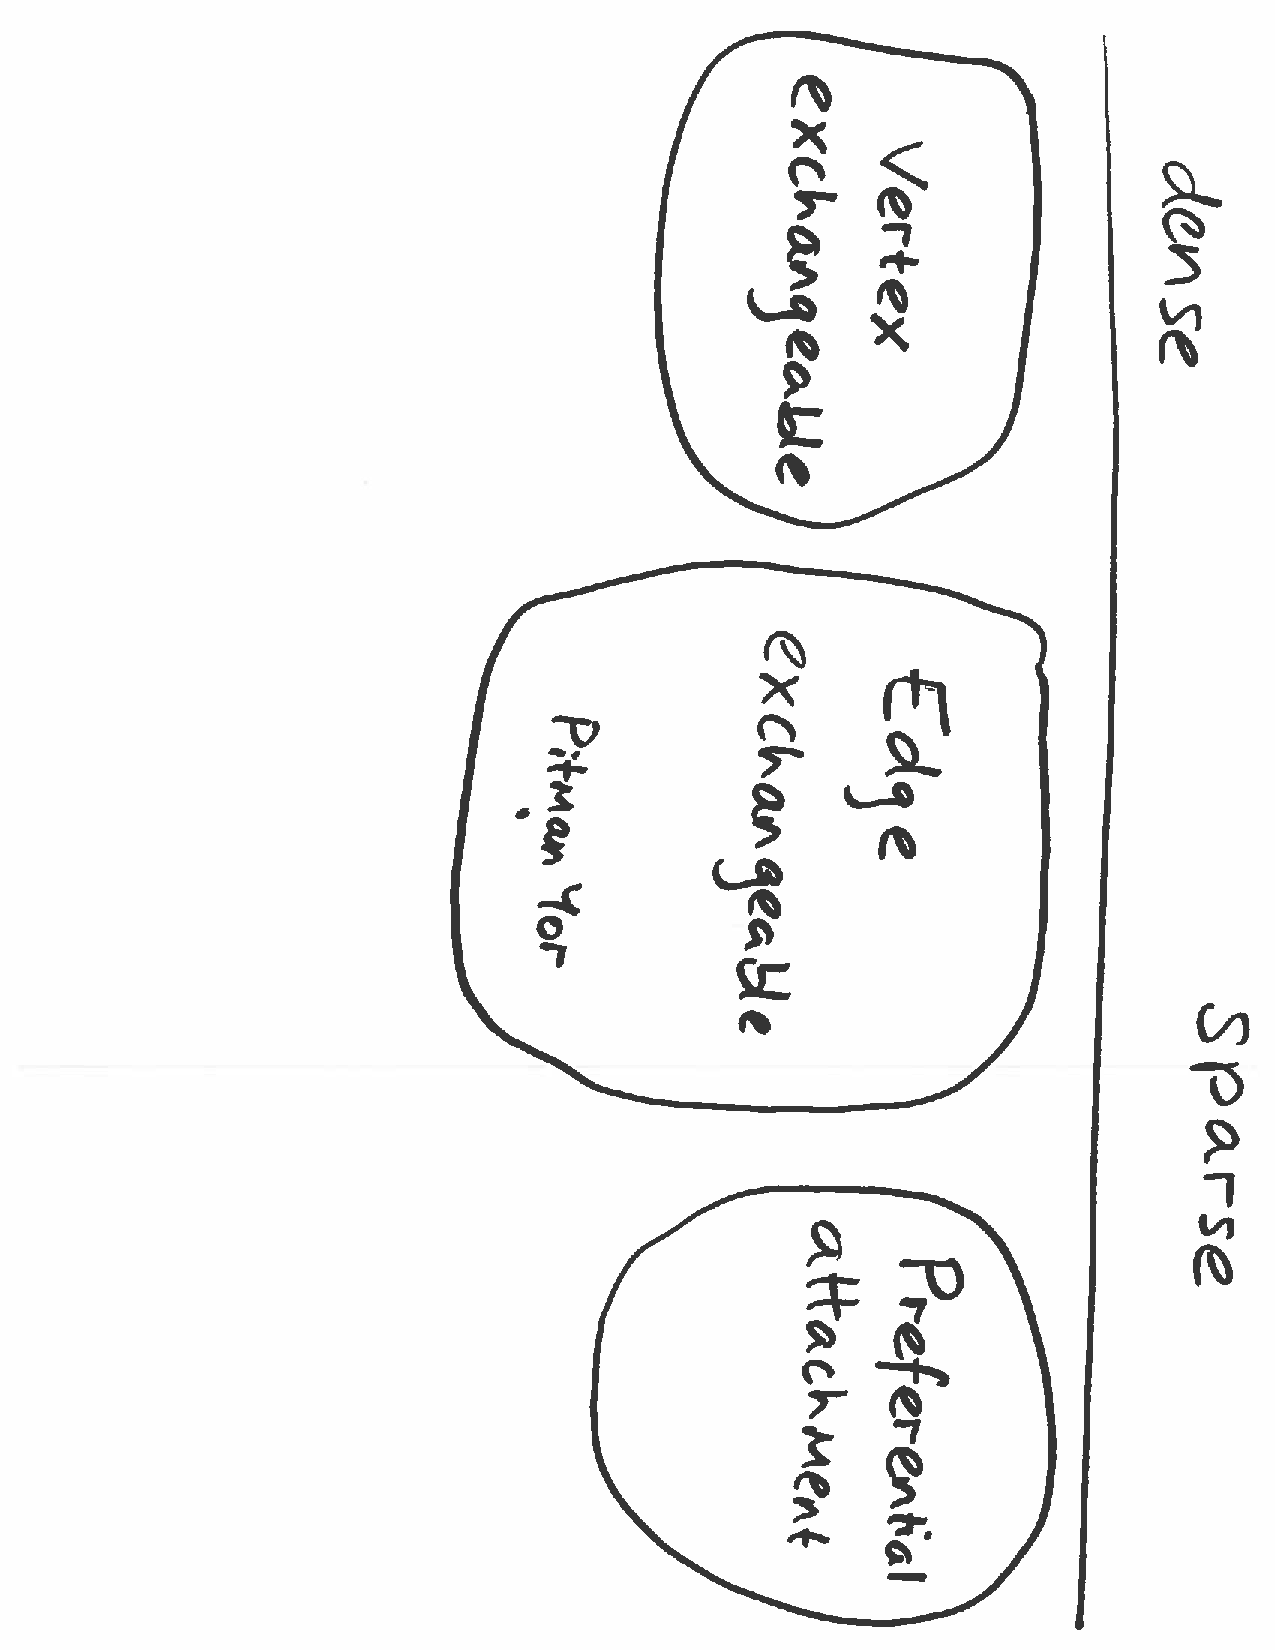
\includegraphics[angle=90,origin=c,scale=0.4]{fig/models4}
\end{frame}

\begin{frame}
	\frametitle{Edge exchangeable models \cite{cai2016}, \cite{CraneDempsey2017}}
	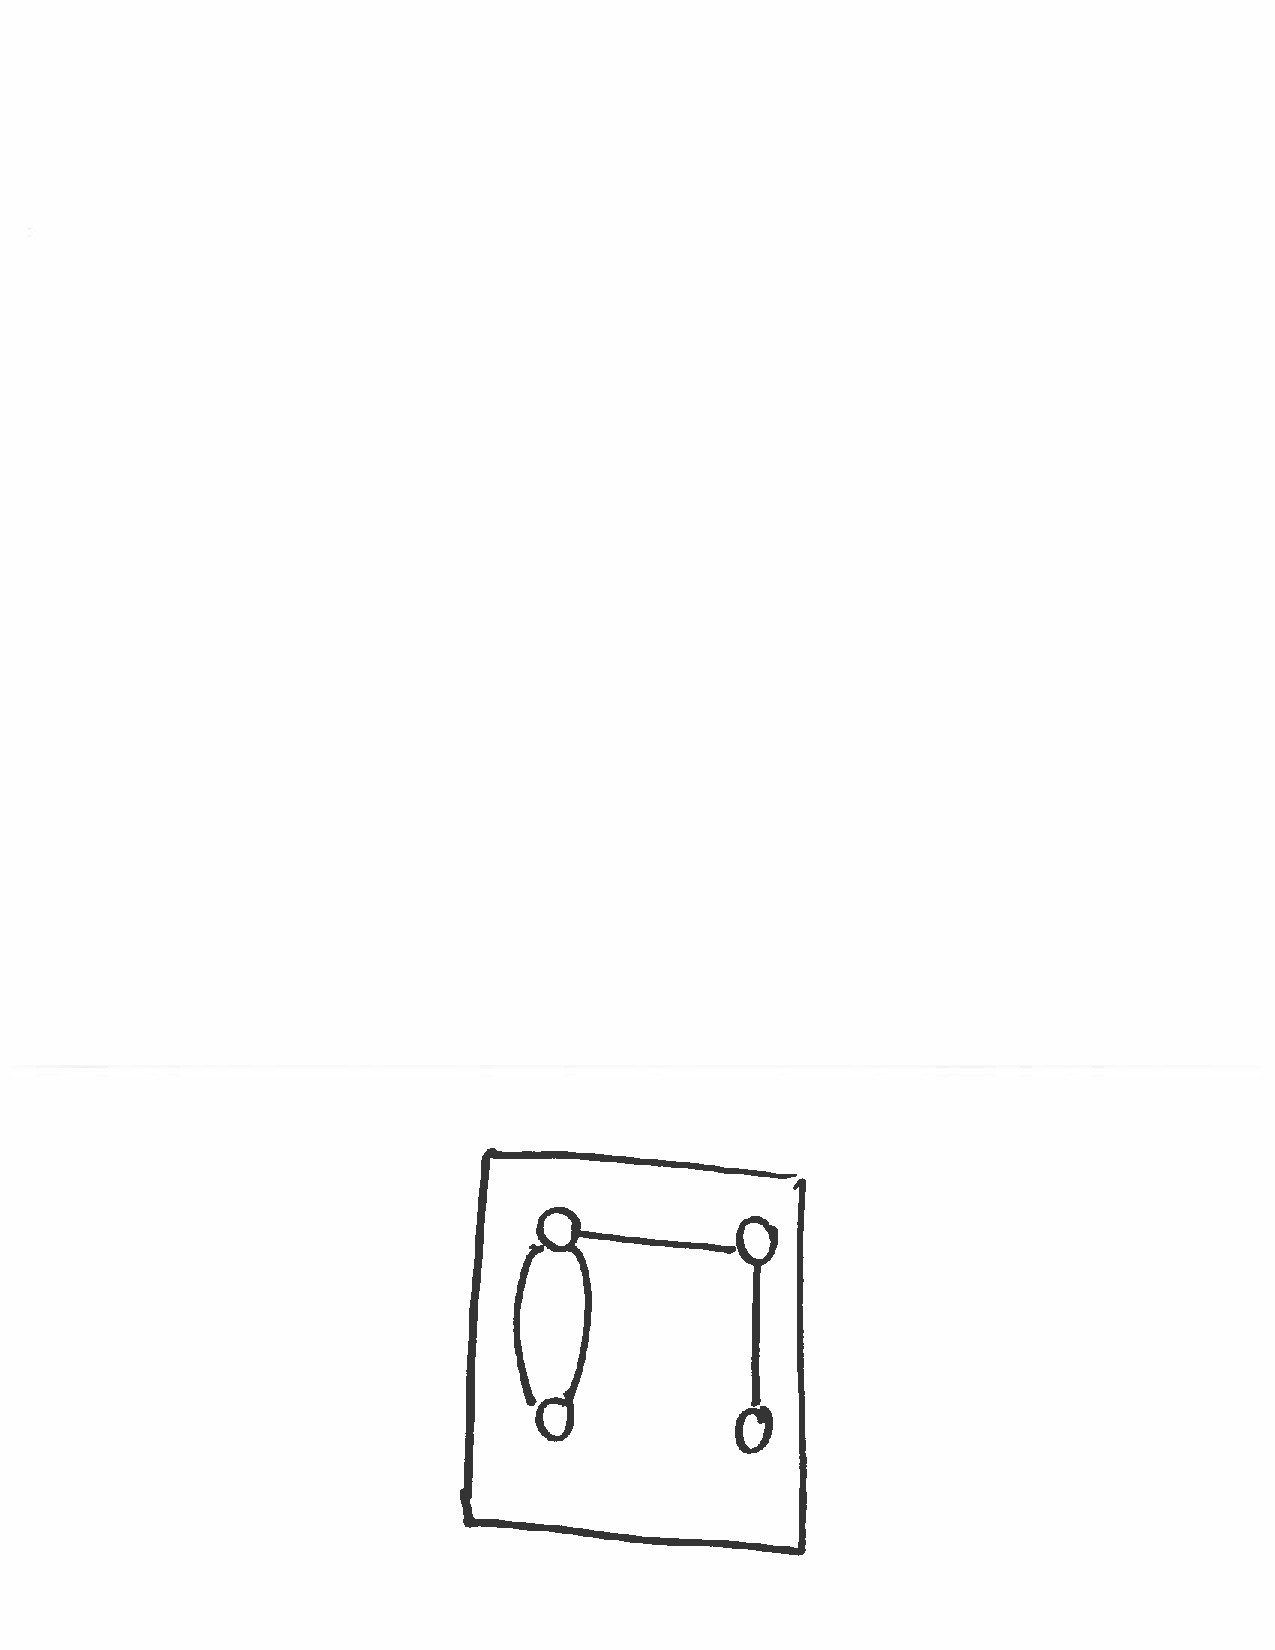
\includegraphics[angle=90,origin=c,scale=0.4]{fig/ee1}
\end{frame}

\begin{frame}
	\frametitle{Edge exchangeable models \cite{cai2016}, \cite{CraneDempsey2017}}
	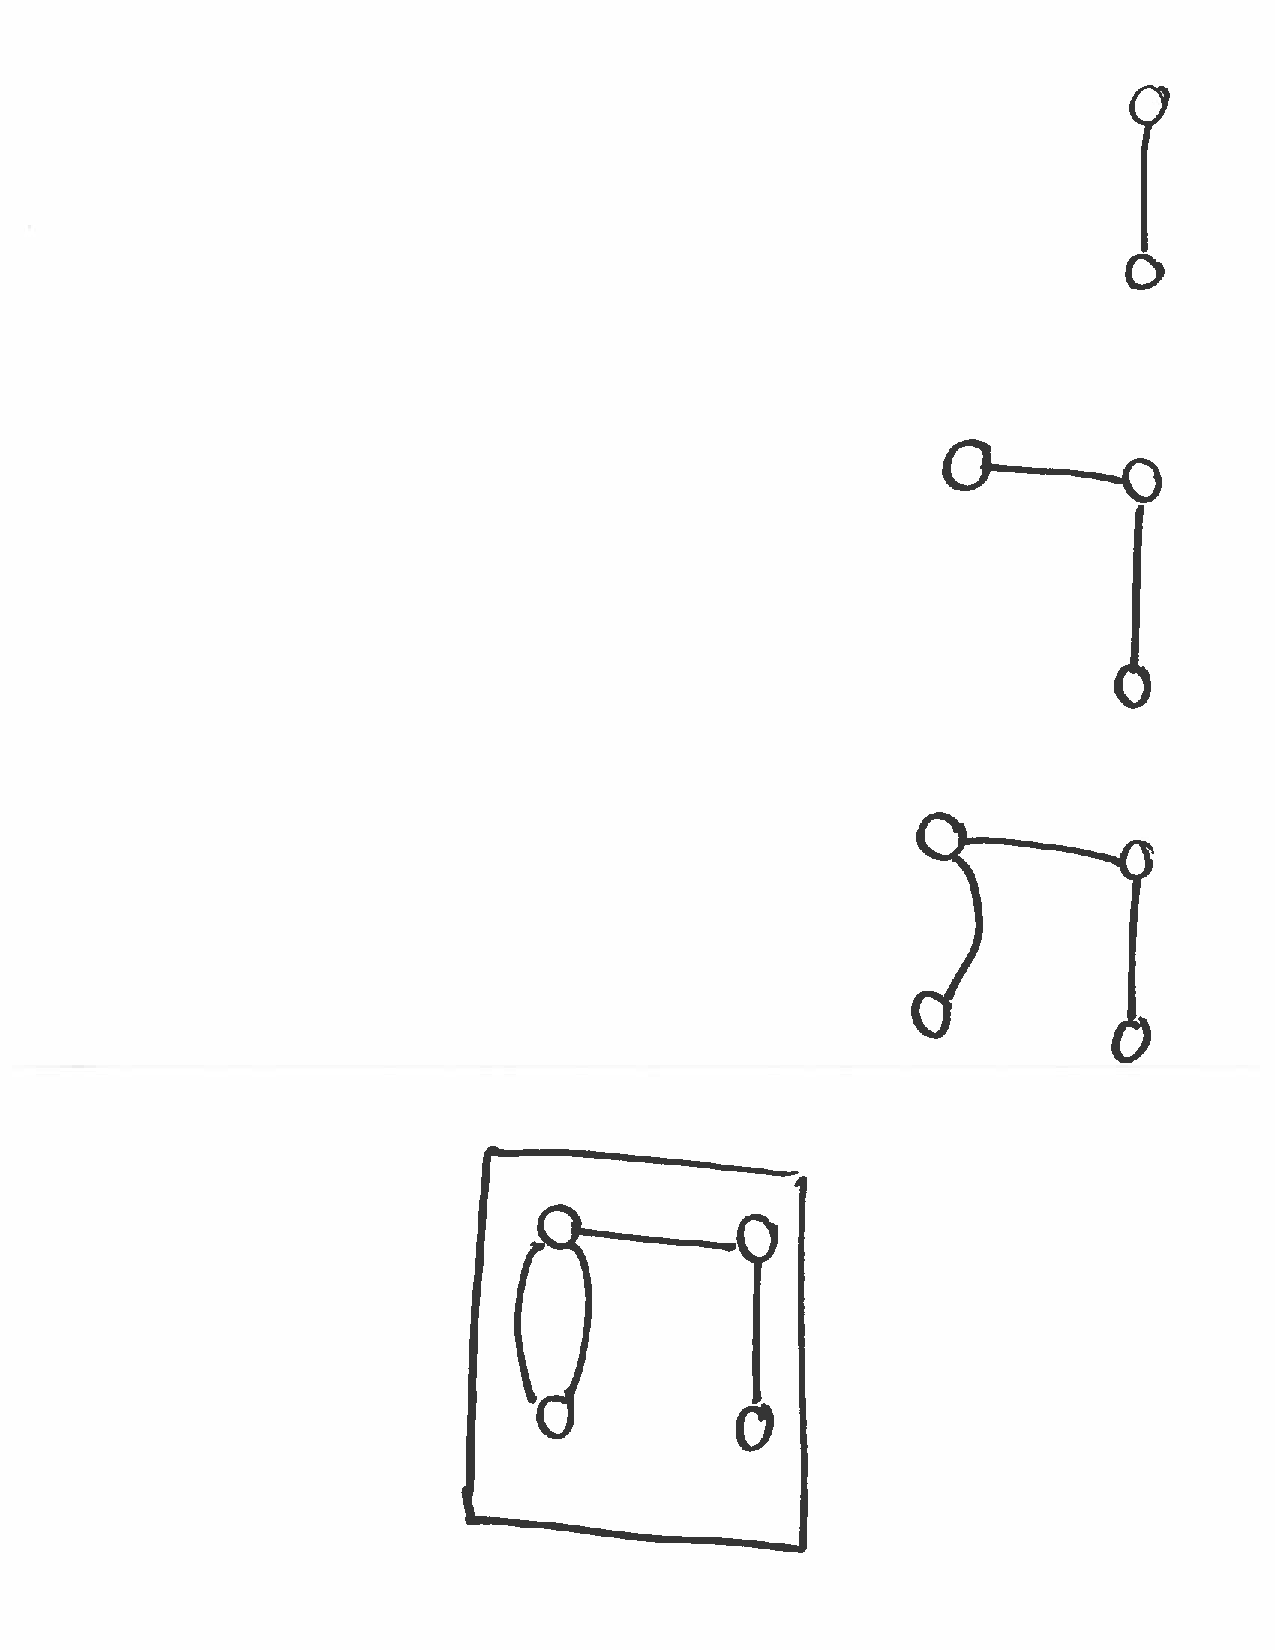
\includegraphics[angle=90,origin=c,scale=0.4]{fig/ee2}
\end{frame}

\begin{frame}
	\frametitle{Edge exchangeable models \cite{cai2016}, \cite{CraneDempsey2017}}
	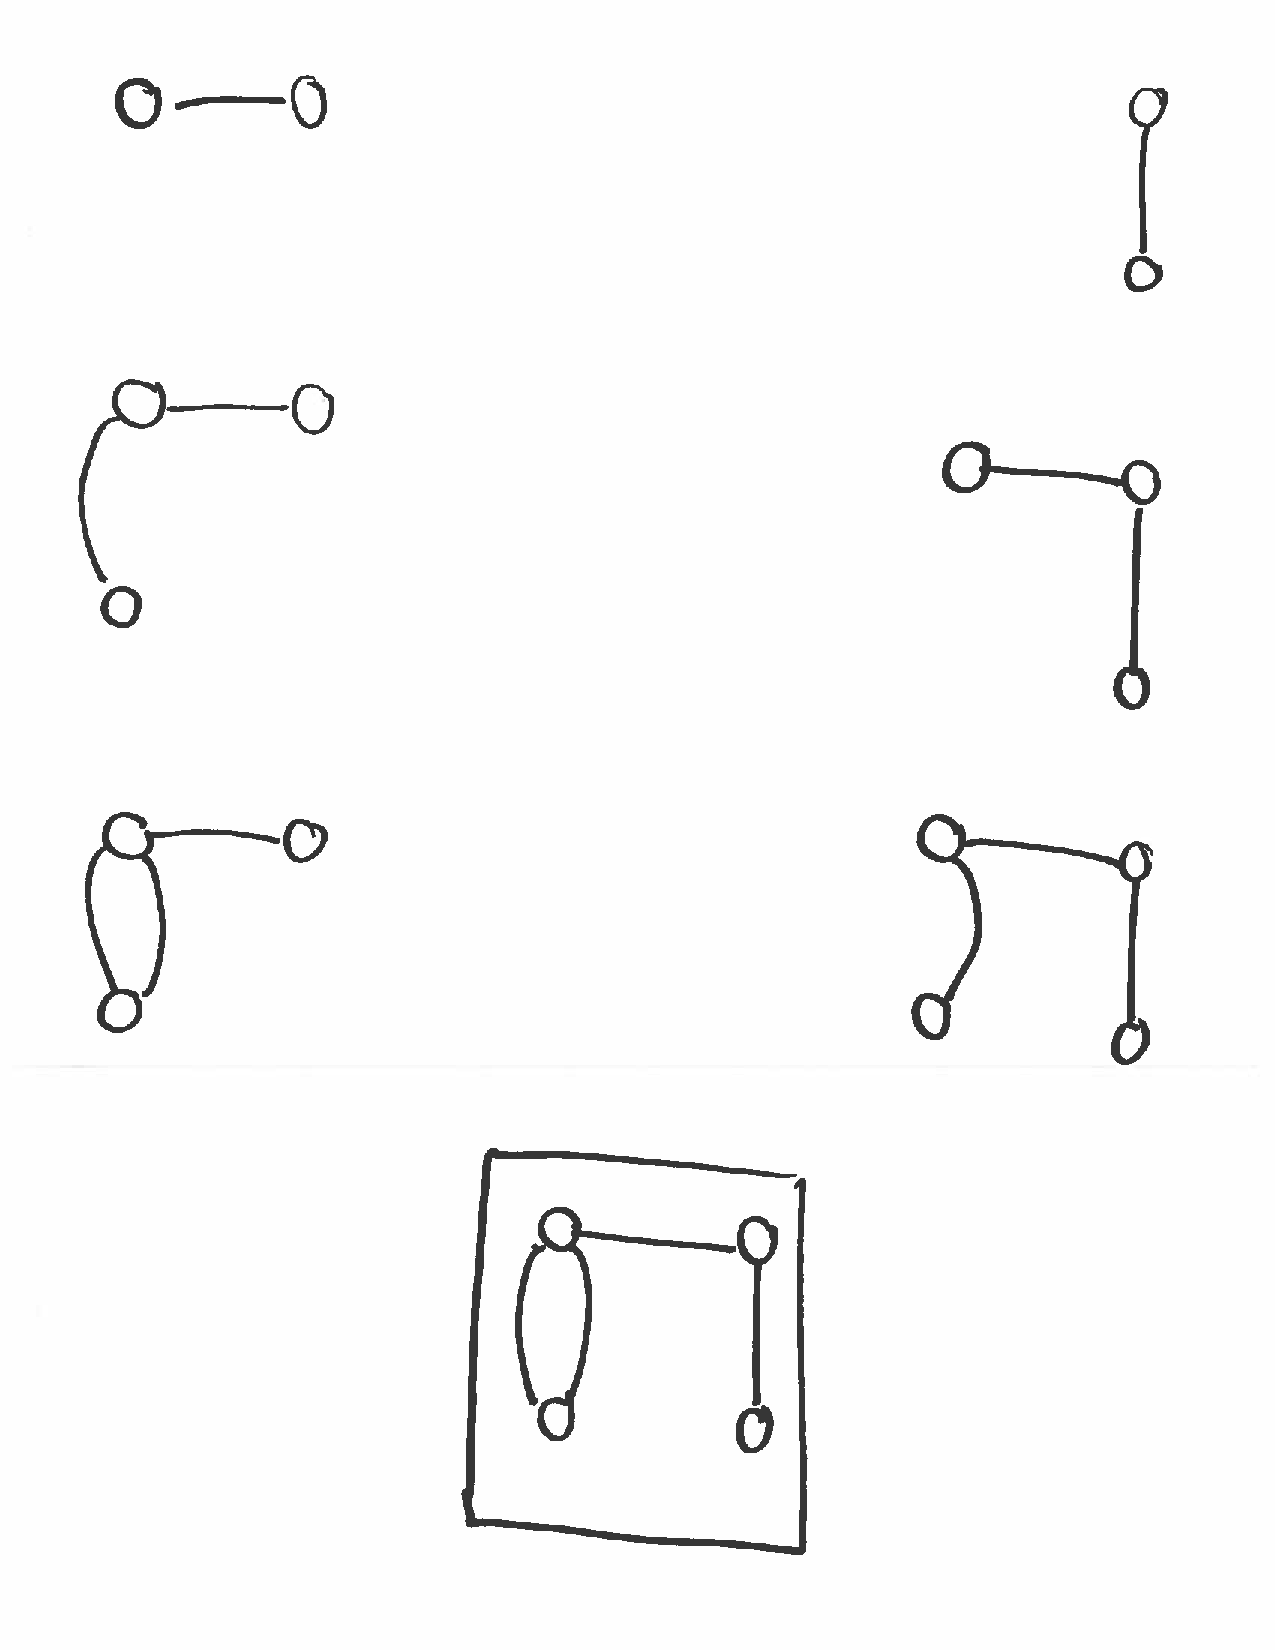
\includegraphics[angle=90,origin=c,scale=0.4]{fig/ee3}
\end{frame}

\begin{frame}
	\frametitle{Factorizable (``rank one'') paintbox representation}
	% 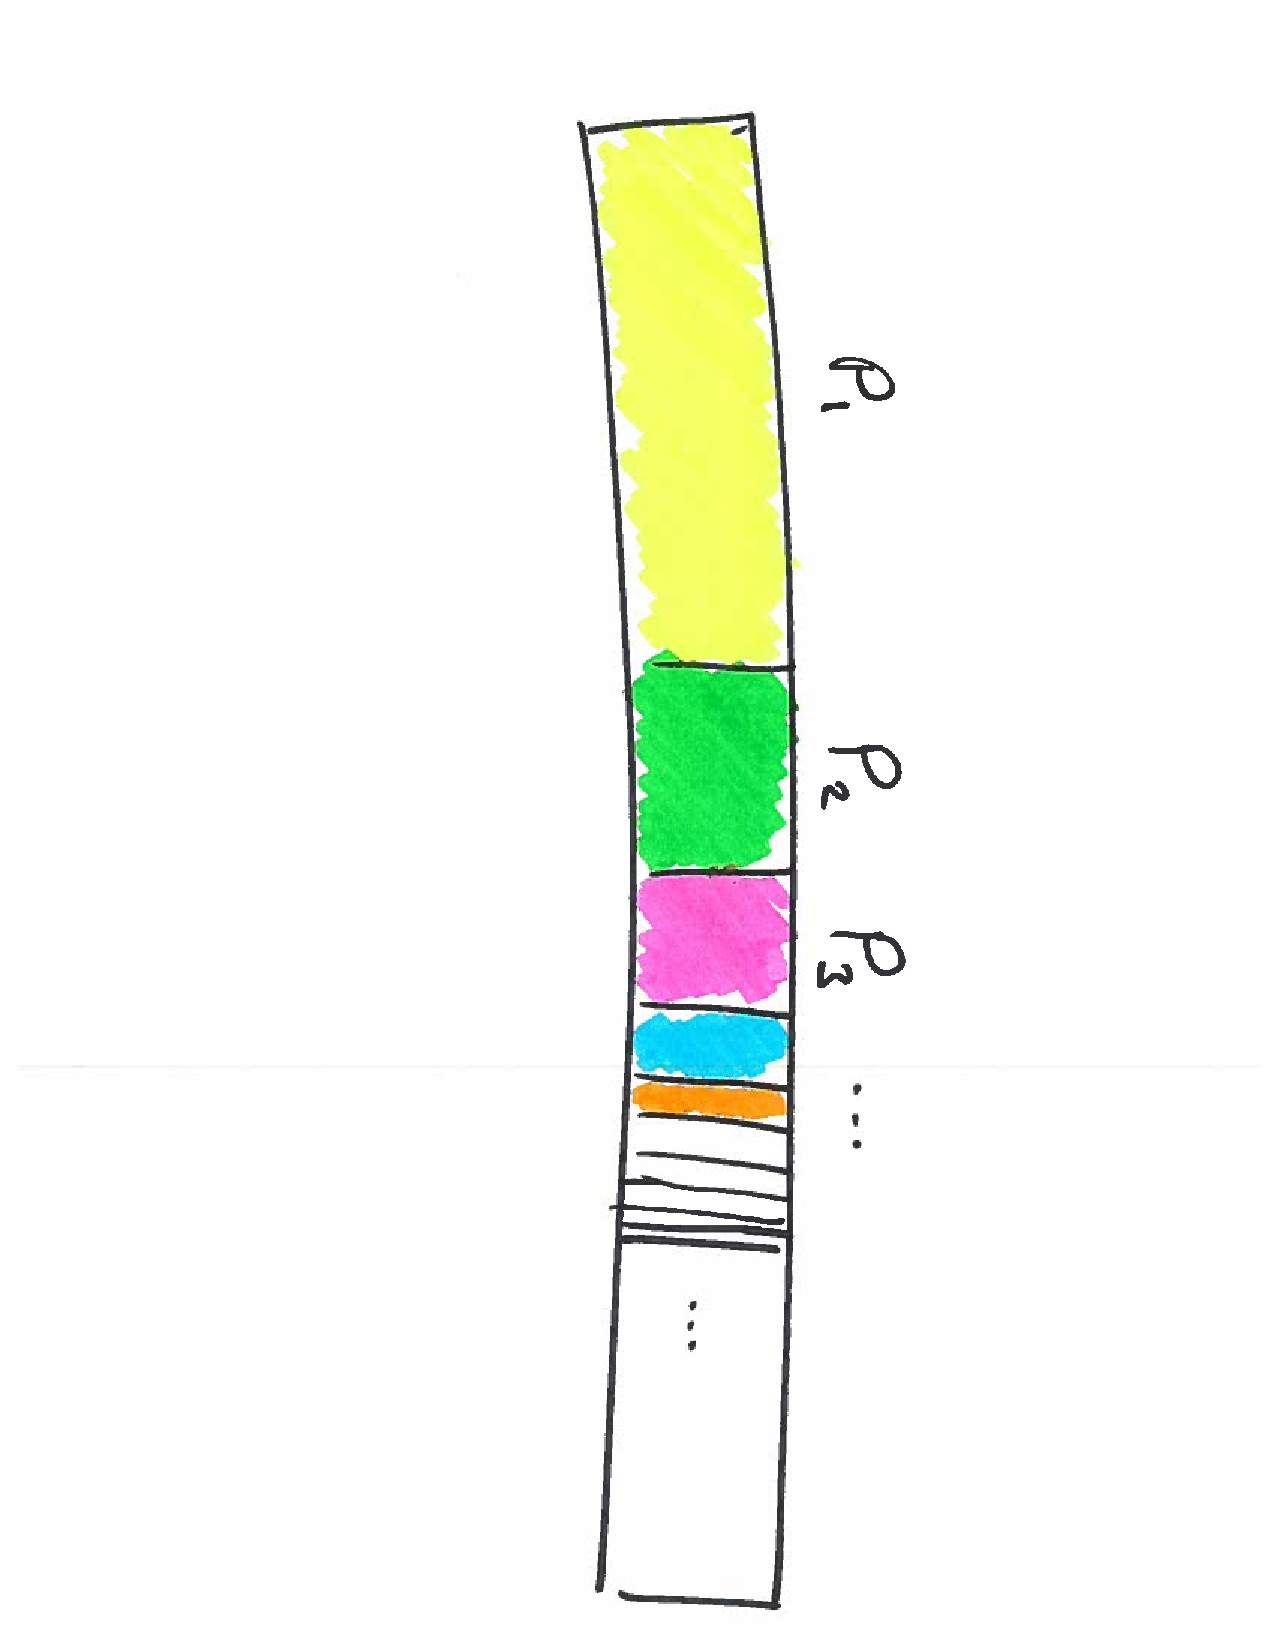
\includegraphics[angle=90,origin=c,scale=0.4]{fig/paintbox}
	\begin{center}
	  \resizebox{\textwidth}{!}{
		\begin{tikzpicture}
			% boundary of paintbox
			\coordinate (origin) at (0,0);
			\coordinate (xmax) at (8,0);
			\coordinate (xymax) at (8,1);
			\coordinate (ymax) at (0,1);
			% dummy to make math work
			\coordinate (yoff) at (0,1);

			% interval x coords
			\coordinate (int1) at (1.75,1);
			\coordinate (int1b) at (1.75,0);
			\coordinate (int2) at (2.75,1);
			\coordinate (int2b) at (2.75,0);
			\coordinate (int3) at (4.1,1);
			\coordinate (int3b) at (4.1,0);
			\coordinate (int4) at (5.1,1);
			\coordinate (int4b) at (5.1,0);
			\coordinate (int5) at (6.0,1);
			\coordinate (int5b) at (6.0,0);
			\coordinate (int6) at (6.7,1);
			\coordinate (int6b) at (6.7,0);
			\coordinate (int7) at (7.4,1);

			% draw paintbox
			\draw (origin) -- (xmax) -- (xymax) -- (ymax) -- cycle;
			\fill[blueClj] (origin) rectangle (int1);
			\fill[orangeClj] (int1b) rectangle (int2);
			\fill[darkgreenClj] (int2b) rectangle (int3);
			\fill[grayClj] (int3b) rectangle (int4);
			\fill[purpleClj] (int4b) rectangle (int5);
			\fill[cyanClj] (int5b) rectangle (int6);
			\fill[redClj] (int6b) rectangle (int7);

			% interval labels
			\node at (origin) [color=darkblue,label=below:{\Large $0$}]{};
			\node at (xmax) [color=darkblue,label=below:{\Large $1$}]{};
			\node at ($0.5*(int1)-0.5*(ymax)+(yoff)$) [color=darkblue,label=above:{\Large $P_1$}]{};
			\node at ($0.5*(int1)+0.5*(int2)$) [color=darkblue,label=above:{\Large $P_2$}]{};
			\node at ($0.5*(int2)+0.5*(int3)$) [color=darkblue,label=above:{\Large $P_3$}]{};
			\node at ($0.5*(int3)+0.5*(int4)$) [color=darkblue,label=above:{\Large $P_4$}]{};
			\node at ($0.5*(int4)+0.5*(int5)$) [color=darkblue,label=above:{\Large $P_5$}]{};
			\node at ($0.5*(int5)+0.5*(int6)$) [color=darkblue,label=above:{\Large $P_6$}]{};
			\node at ($0.5*(int6)+0.5*(int7)$) [color=darkblue,label=above:{\Large $P_7$}]{};
			\node at ($0.5*(int7)+0.5*(xymax)$) [color=darkblue,label=above:{\Large $\dotsc$}]{};

			% uniform r.v.'s
			\foreach \x/\xn/\xco in {3.0/1/darkgrayClj, 6.4/2/darkgrayClj, 1.3/3/darkgrayClj, 5.3/4/darkgrayClj,0.6/5/darkgrayClj,7.1/6/darkgrayClj}
			{
				\fill[color=\xco] (\x,-1.0) circle (2pt) node[anchor=north,color=darkblue]{$U_{\xn}$} ;
				\draw[dashed,color=darkblue] ($(\x,-1.0)+(0,0.1)$) -- (\x,1.25);
			}

		\end{tikzpicture}
	  }
	  Sequence of edges: $((3,6),(1,5),(1,7))$
	  \vspace{0.5cm}

	  \only<2>{
	    \resizebox{0.75\textwidth}{!}{
		  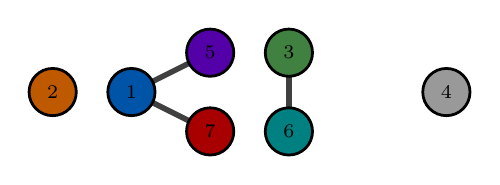
\begin{tikzpicture}
			% vertices
		  	\Vertex[label=1, color=blueClj, x=0, y=0]{v1}
		  	\Vertex[label=2, color=orangeClj, x=-1, y=0]{v2}
		  	\Vertex[label=3, color=darkgreenClj, x=2, y=0.5]{v3}
		  	\Vertex[label=4, color=grayClj, x=4, y=0]{v4}
		  	\Vertex[label=5, color=purpleClj, x=1, y=0.5]{v5}
		  	\Vertex[label=6, color=cyanClj, x=2, y=-0.5]{v6}
		  	\Vertex[label=7, color=redClj, x=1, y=-0.5]{v7}

		  	% edges
		  	\Edge[lw=2](v3)(v6)
		  	\Edge[lw=2](v1)(v5)
		  	\Edge[lw=2](v1)(v7)
		  \end{tikzpicture}
	    }
	  }
	\end{center}
\end{frame}

\begin{frame}
	\frametitle{Paintbox representation}
	Consequences for edge exchangeable models:
	\begin{itemize}
		\item Rate of vertex arrival gets slower and slower \\
			$\Rightarrow$ sublinear sparsity: \#vertices $=o(\text{\#edges})$
		\item Edges pile up \\
			$\Rightarrow$ linear scaling of degrees: $d_{j,n}=\Theta(n)$
	\end{itemize}
\end{frame}

\begin{frame}
	\frametitle{Models}
	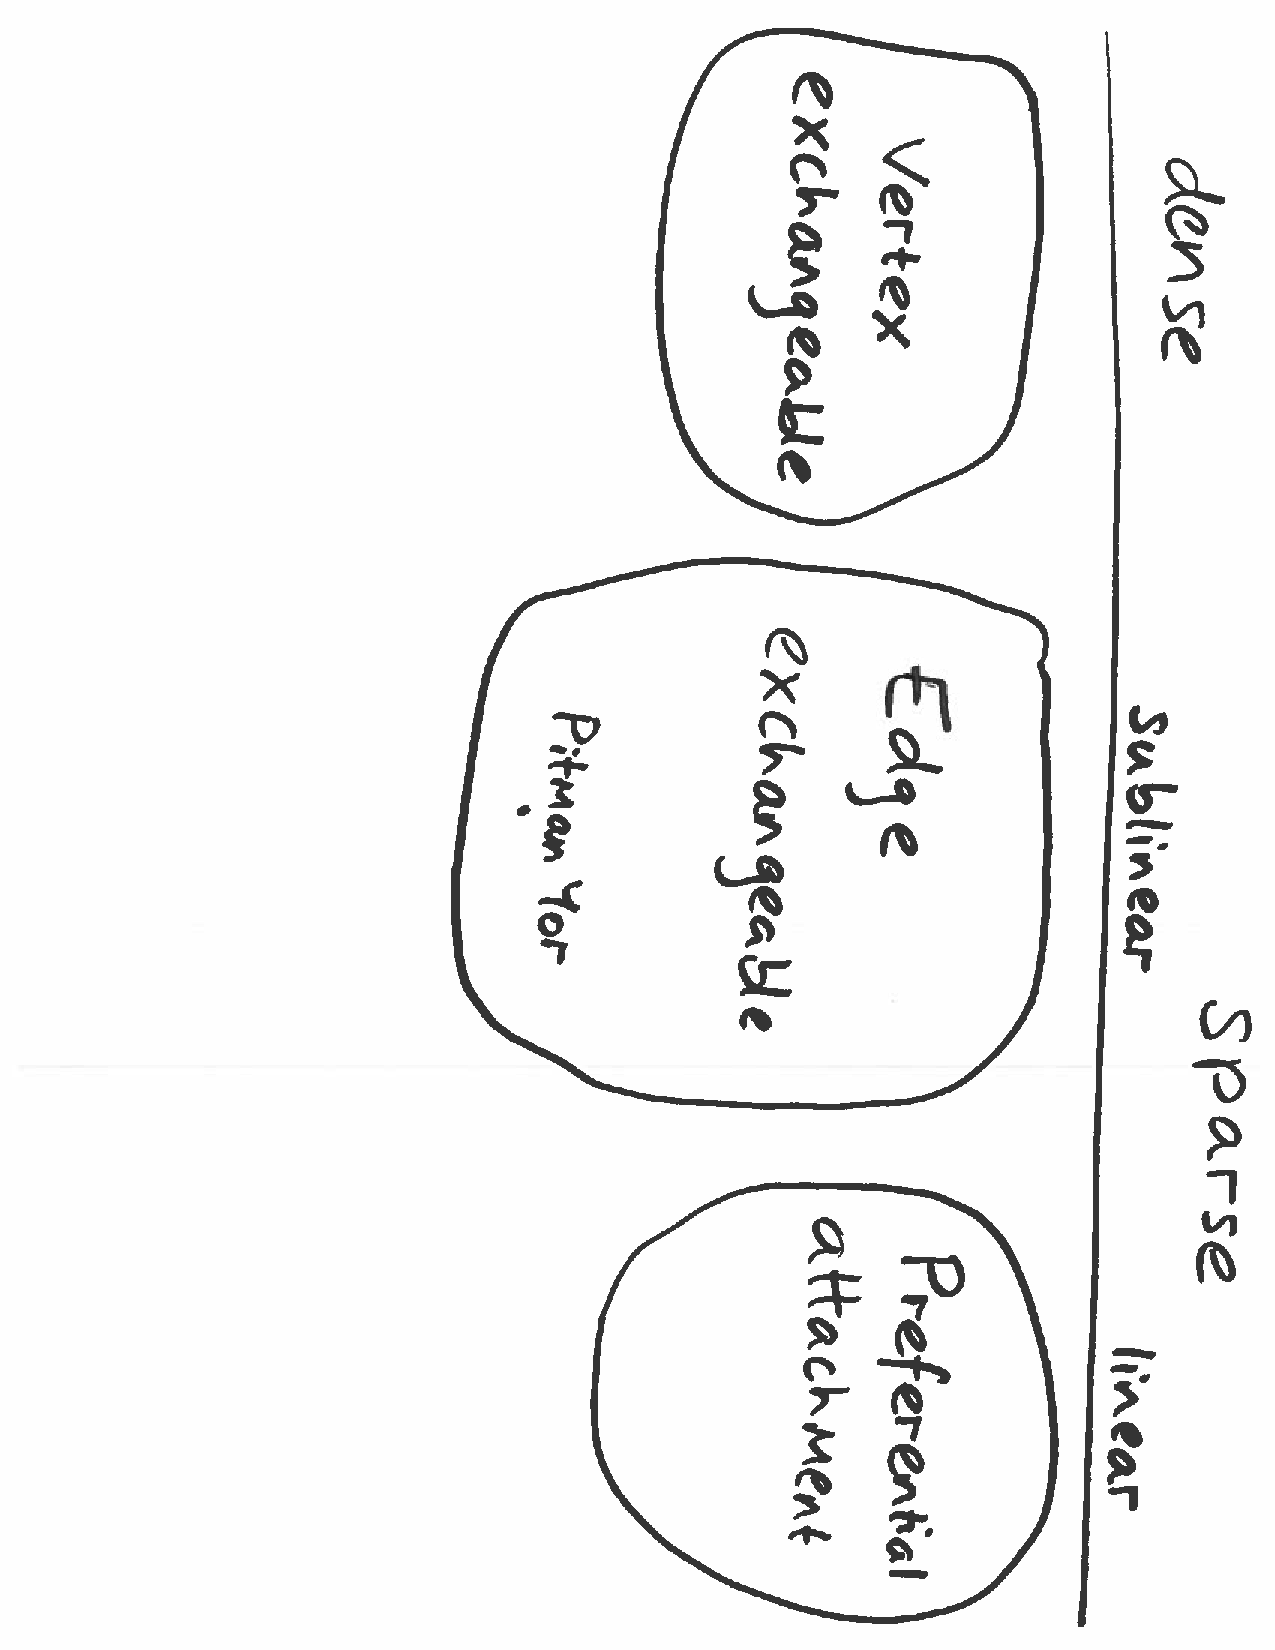
\includegraphics[angle=90,origin=c,scale=0.4]{fig/models5}
\end{frame}

\begin{frame}
	\frametitle{Models}
	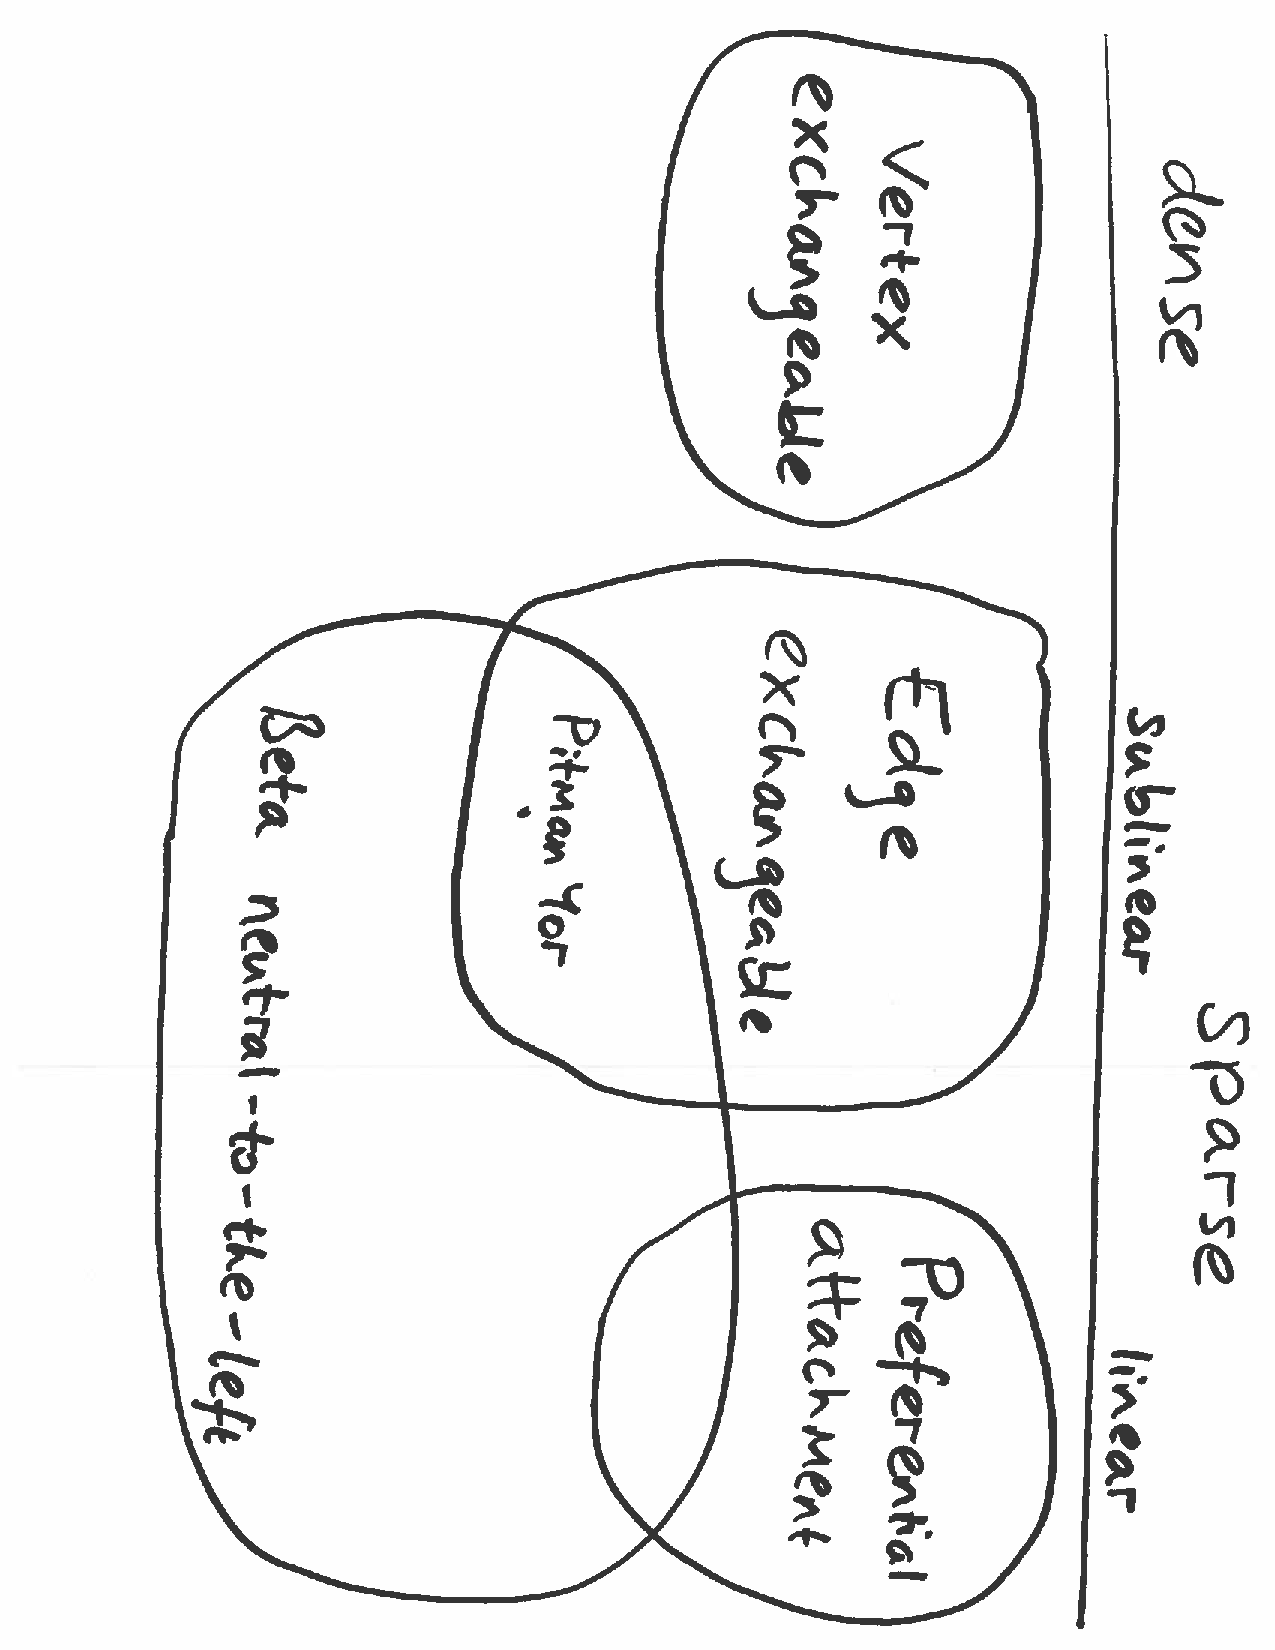
\includegraphics[angle=90,origin=c,scale=0.4]{fig/models6}
\end{frame}

\begin{frame}
	\frametitle{Models}
	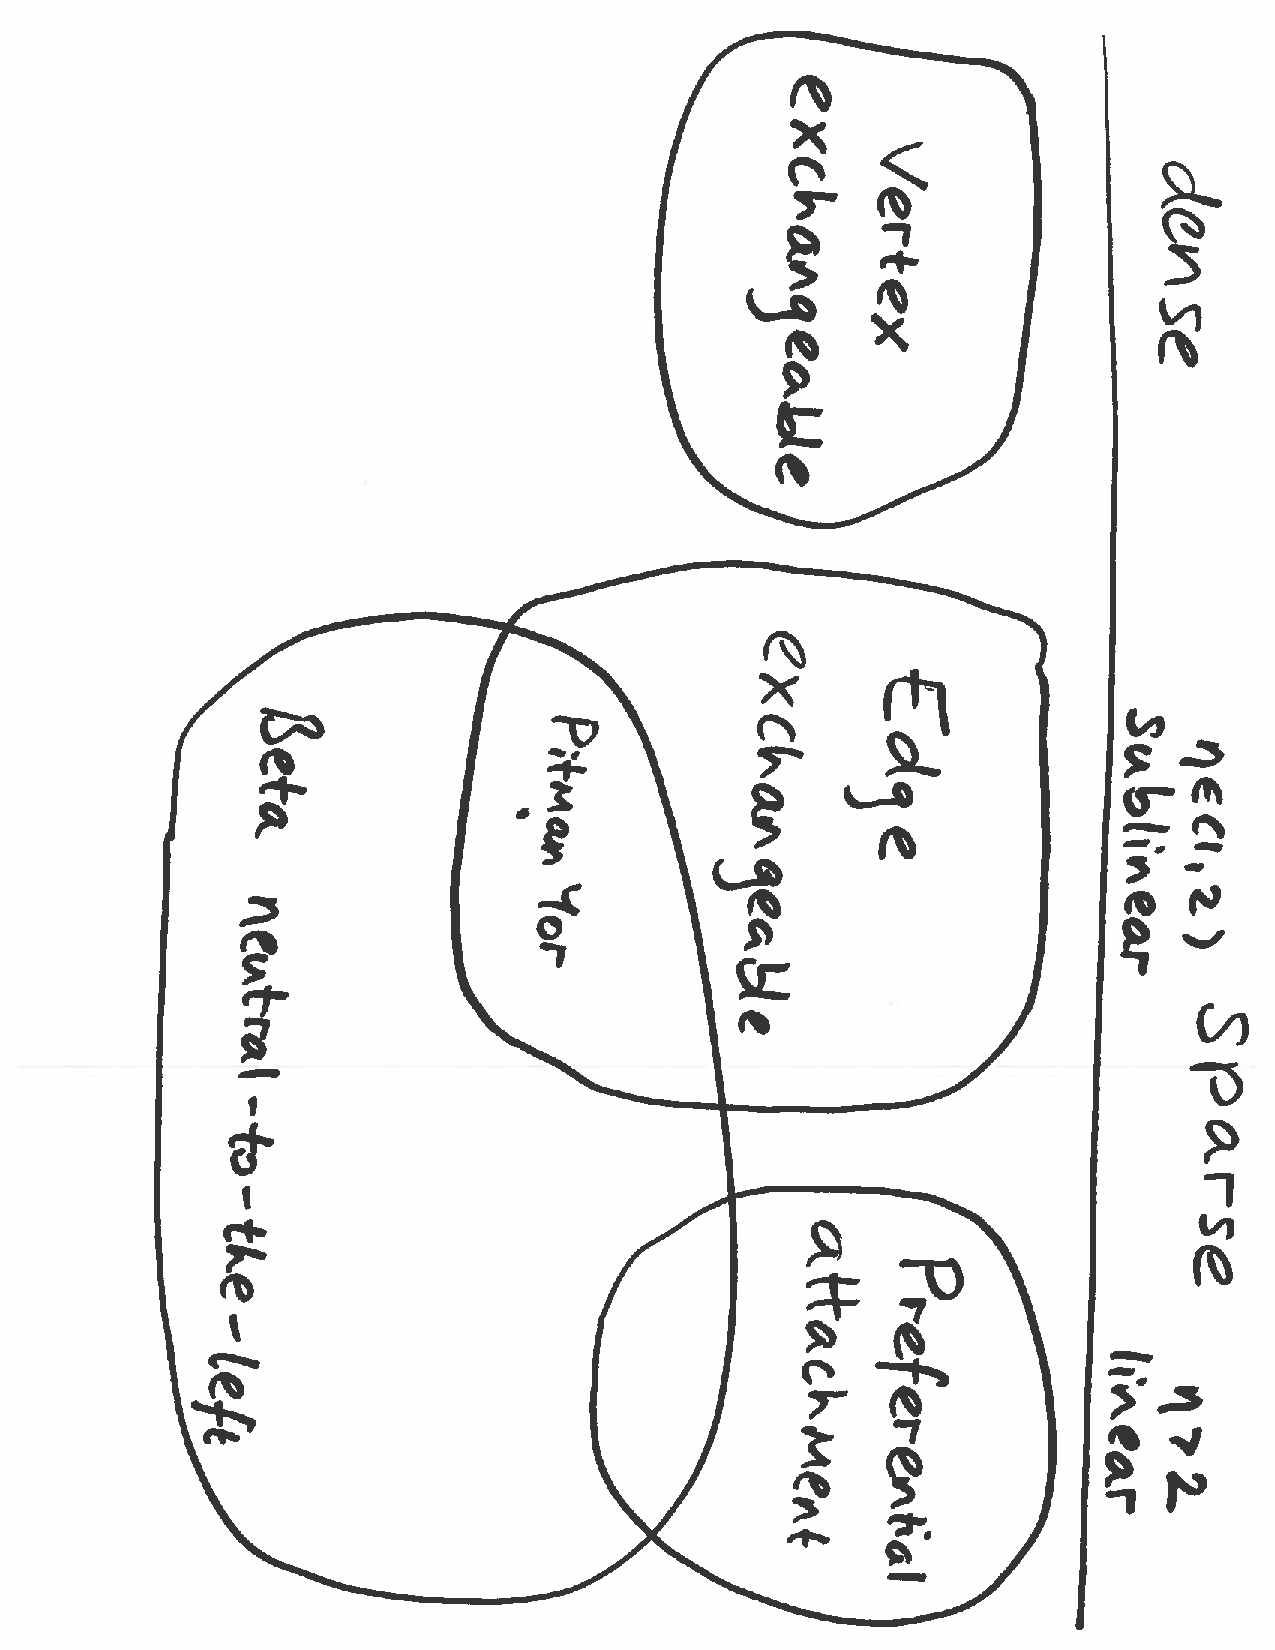
\includegraphics[angle=90,origin=c,scale=0.4]{fig/models7}
\end{frame}

\begin{frame}
	\frametitle{Beta Neutral-to-the-left Model \cite{Bloem2017}}
	% \vspace{2pt}
	% 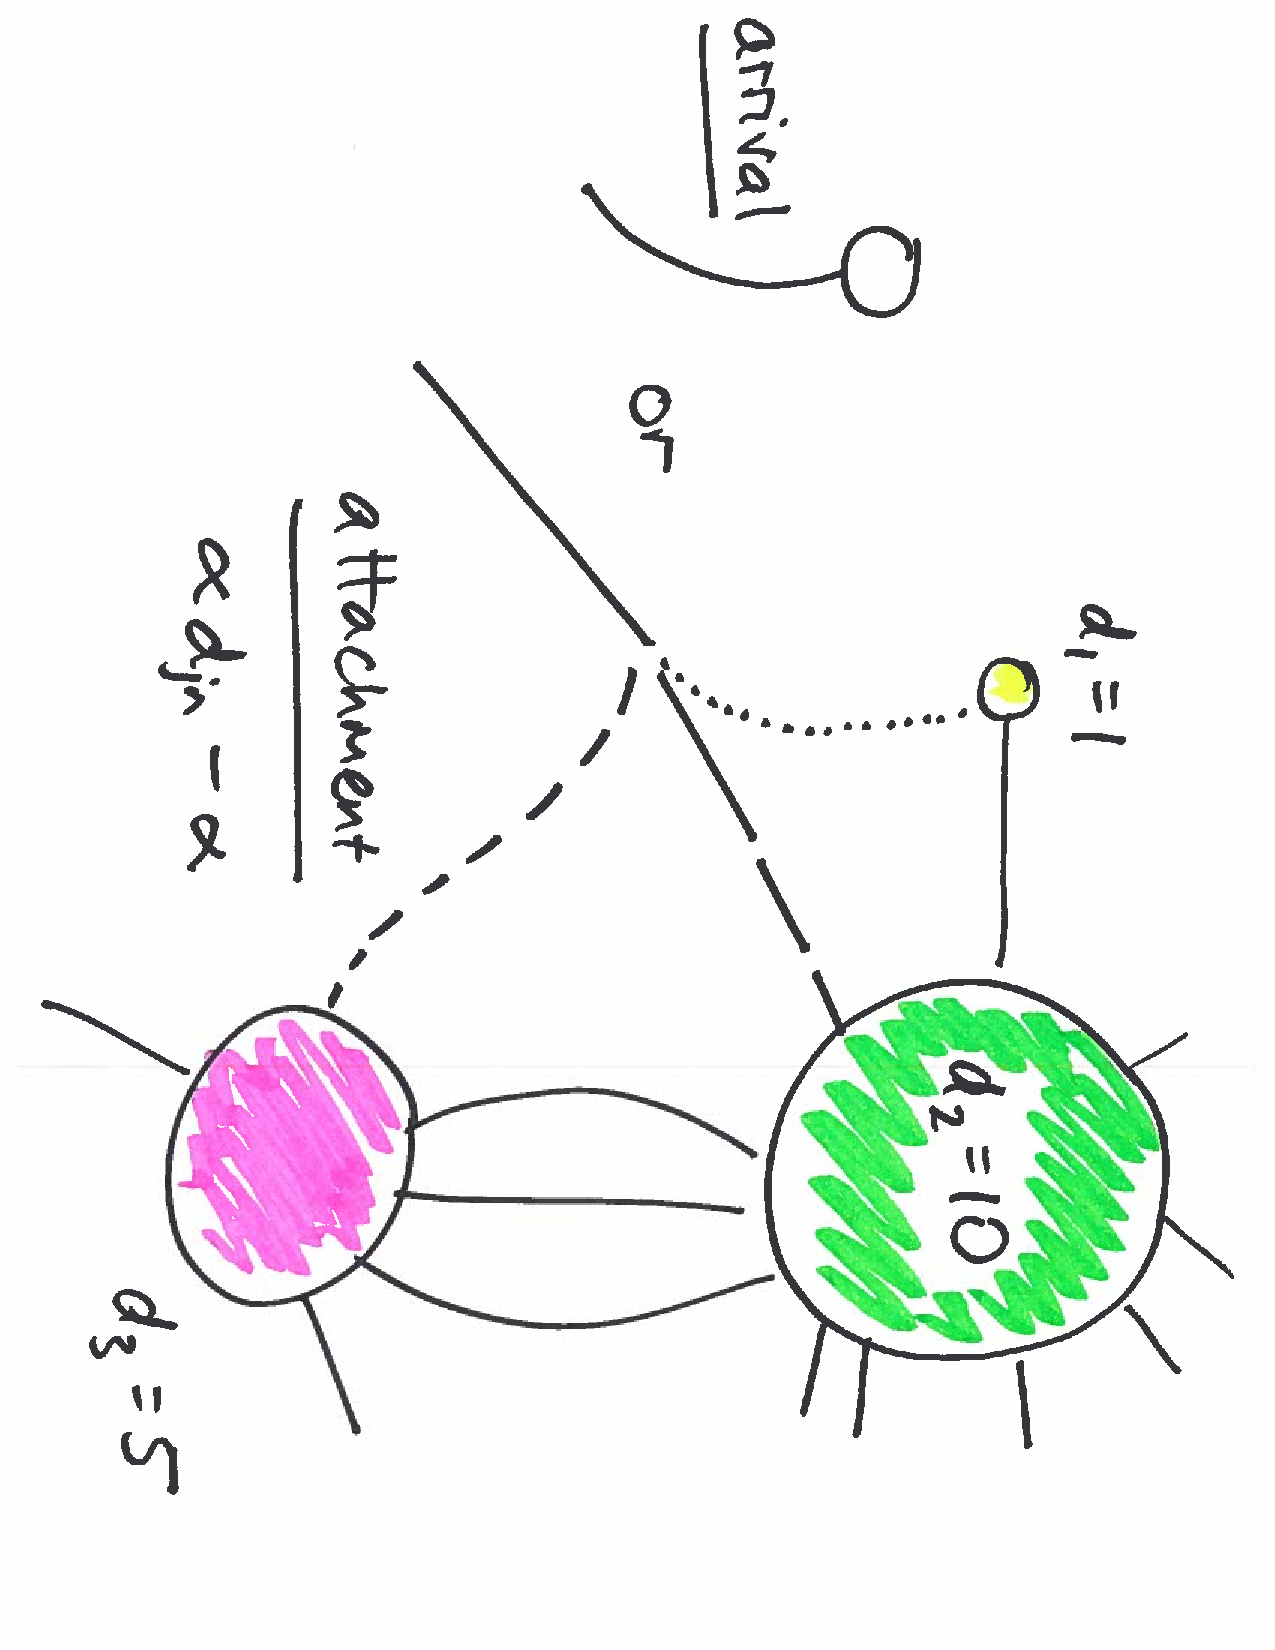
\includegraphics[angle=90,origin=c,scale=0.37]{fig/bntl}
	\begin{enumerate}
		\item Generate arrival times $1=T_1< T_2 < T_3 < \dotsc$ in any way.
		\item Generate ends of edges sequentially:
	\end{enumerate}
	\begin{center}
	\makebox[\textwidth][c]{
	  \resizebox{1.1\textwidth}{!}{
		\begin{tikzpicture}
			% G_n
			\Vertex[size=0.5,color=blueClj,x=0,y=0]{v1}
			\Vertex[size=0.5,color=orangeClj,x=2,y=0]{v2}
			\Vertex[size=0.5,color=darkgreenClj,x=1,y=1]{v3}
			\Vertex[size=0.5,color=grayClj,x=1,y=-1.2]{v4}
			\Vertex[Pseudo,label={\Large ?},x=1,y=-0.4]{ps}
			\Edge[lw=2](v1)(v2)
			\Edge[lw=2,loopposition=180](v1)(v1)
			\Edge[lw=2,bend=30](v2)(v3)
			\Edge[lw=2,bend=-30](v2)(v3)
			\Edge[lw=2,bend=60](v4)(ps)
			\Text[x=3,y=0]{\Large $G_n$}

			% split on arrival time
			\Text[x=1,y=-2]{Is the next arrival time equal to $n+1$?}
			\Vertex[x=1,y=-2,Pseudo]{vtext}
			\Vertex[x=-1,y=-3,Pseudo,label={\normalsize yes}]{vyes}
			\Vertex[x=3,y=-3,Pseudo,label={\normalsize no}]{vno}
			\Edge[Direct,color=darkblue,bend=20](vtext)(vyes)
			\Edge[Direct,color=darkblue,bend=-20](vtext)(vno)

			% G_{n+1} with new vertex
			\Vertex[size=0.5,color=blueClj,x=-4,y=-4]{v1n}
			\Vertex[size=0.5,color=orangeClj,x=-2,y=-4]{v2n}
			\Vertex[size=0.5,color=darkgreenClj,x=-3,y=-3]{v3n}
			\Vertex[size=0.5,color=grayClj,x=-3,y=-5]{v4n}
			\Vertex[size=0.5,color=purpleClj,x=-4,y=-5]{v5n}
			\Edge[lw=2](v1n)(v2n)
			\Edge[lw=2,loopposition=180](v1n)(v1n)
			\Edge[lw=2,bend=30](v2n)(v3n)
			\Edge[lw=2,bend=-30](v2n)(v3n)
			\Edge[lw=2,bend=60](v4n)(v5n)
			\Text[x=-5.5,y=-4]{\Large $G_{n+1}$}
			\Text[x=-3,y=-6]{\Large $\text{New vertex}$}

			% G_{n+1} without new vertex
			\Vertex[size=0.5,color=blueClj,x=4,y=-4]{v1nn}
			\Vertex[size=0.5,color=orangeClj,x=6,y=-4]{v2nn}
			\Vertex[size=0.5,color=darkgreenClj,x=5,y=-3]{v3nn}
			\Vertex[size=0.5,color=grayClj,x=5,y=-5]{v4nn}
			% \Vertex[size=0.5,color=purpleClj,x=-4,y=-5.2]{v5n}
			\Edge[lw=2](v1nn)(v2nn)
			\Edge[lw=2,loopposition=180](v1nn)(v1nn)
			\Edge[lw=2,bend=30](v2nn)(v3nn)
			\Edge[lw=2,bend=-30](v2nn)(v3nn)
			\Edge[lw=2](v4nn)(v2nn)
			\Text[x=7,y=-4]{\Large $G_{n+1}$}
			\Text[x=5,y=-6]{\Large $\prob[\rightarrow j] \propto \text{deg}_{j,n}-\alpha$}

		\end{tikzpicture}
	  }
	}
	\end{center}
\end{frame}

%\begin{frame}
%	\frametitle{Hierarchical representation of BNTL process}
%	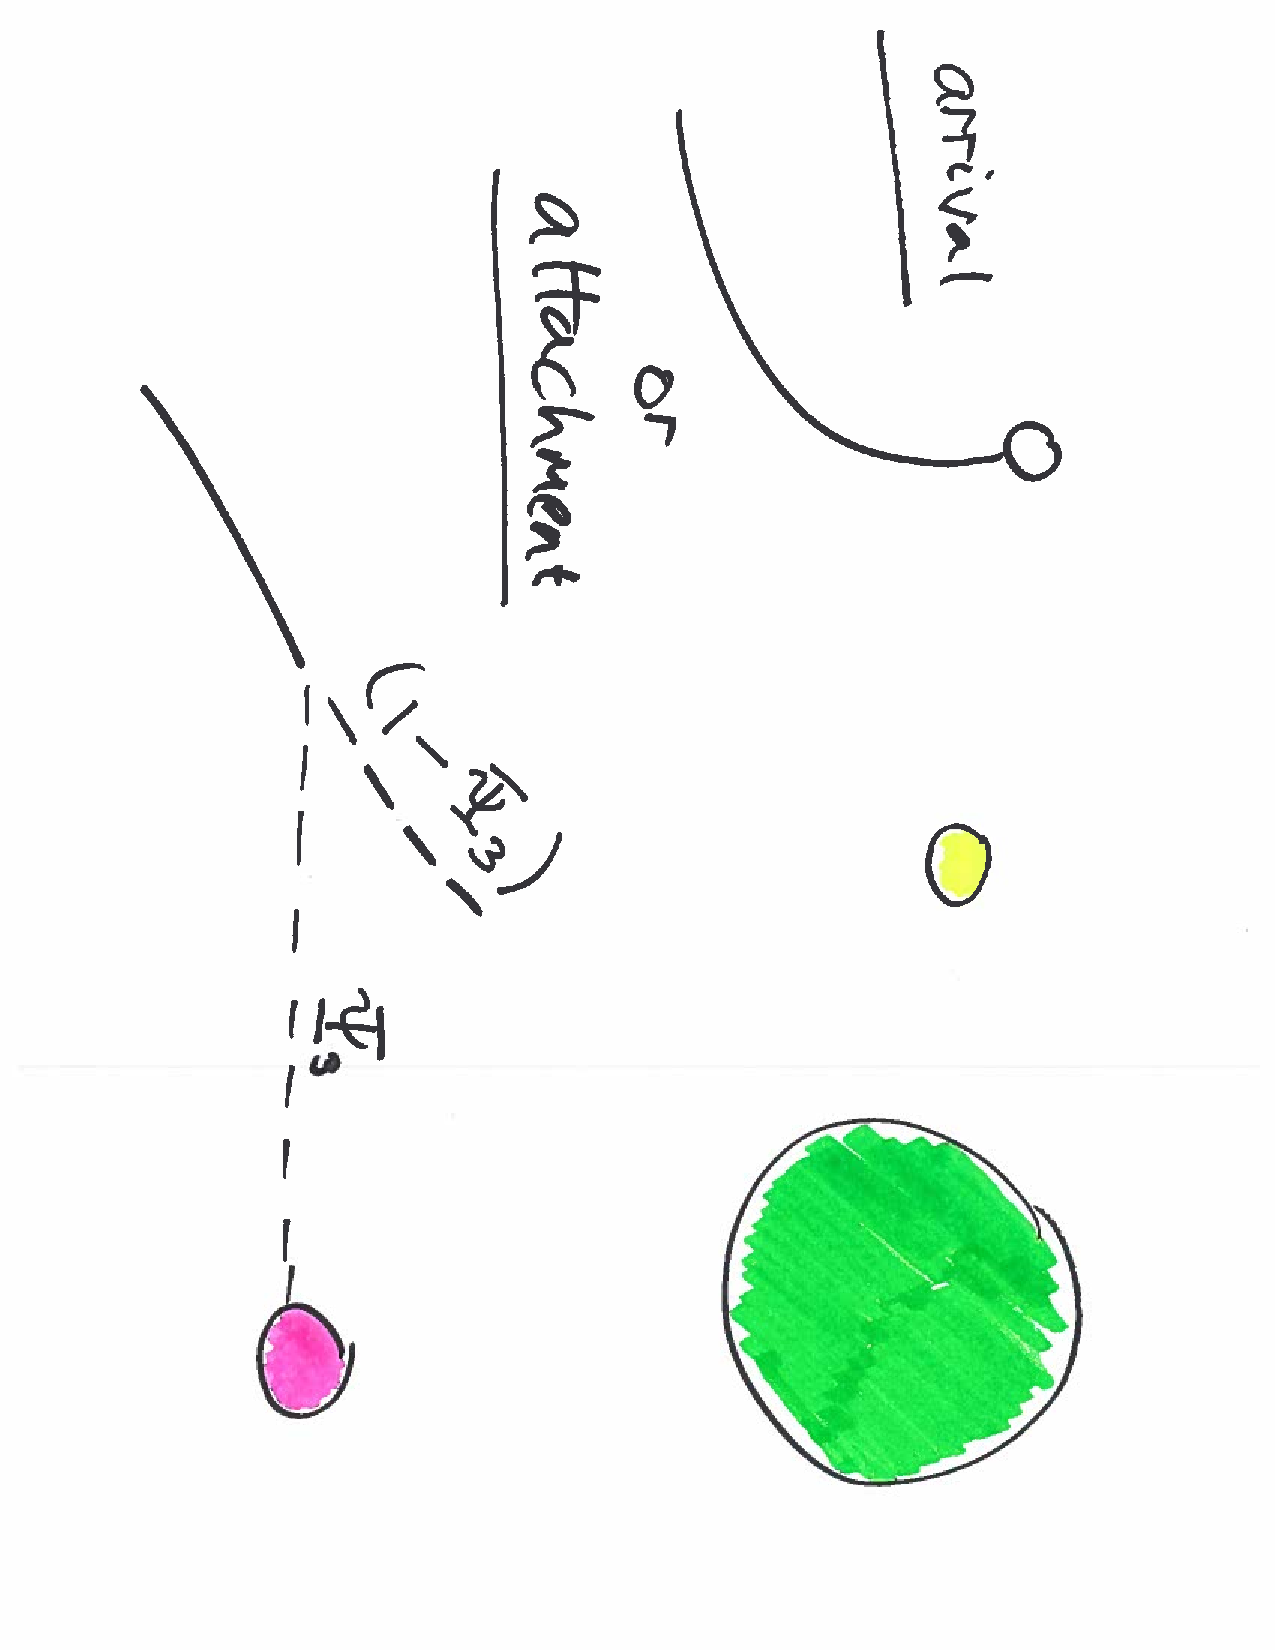
\includegraphics[angle=90,origin=c,scale=0.4]{fig/bntllatent1}
%\end{frame}
%
%\begin{frame}
%	\frametitle{Hierarchical representation of BNTL process}
%	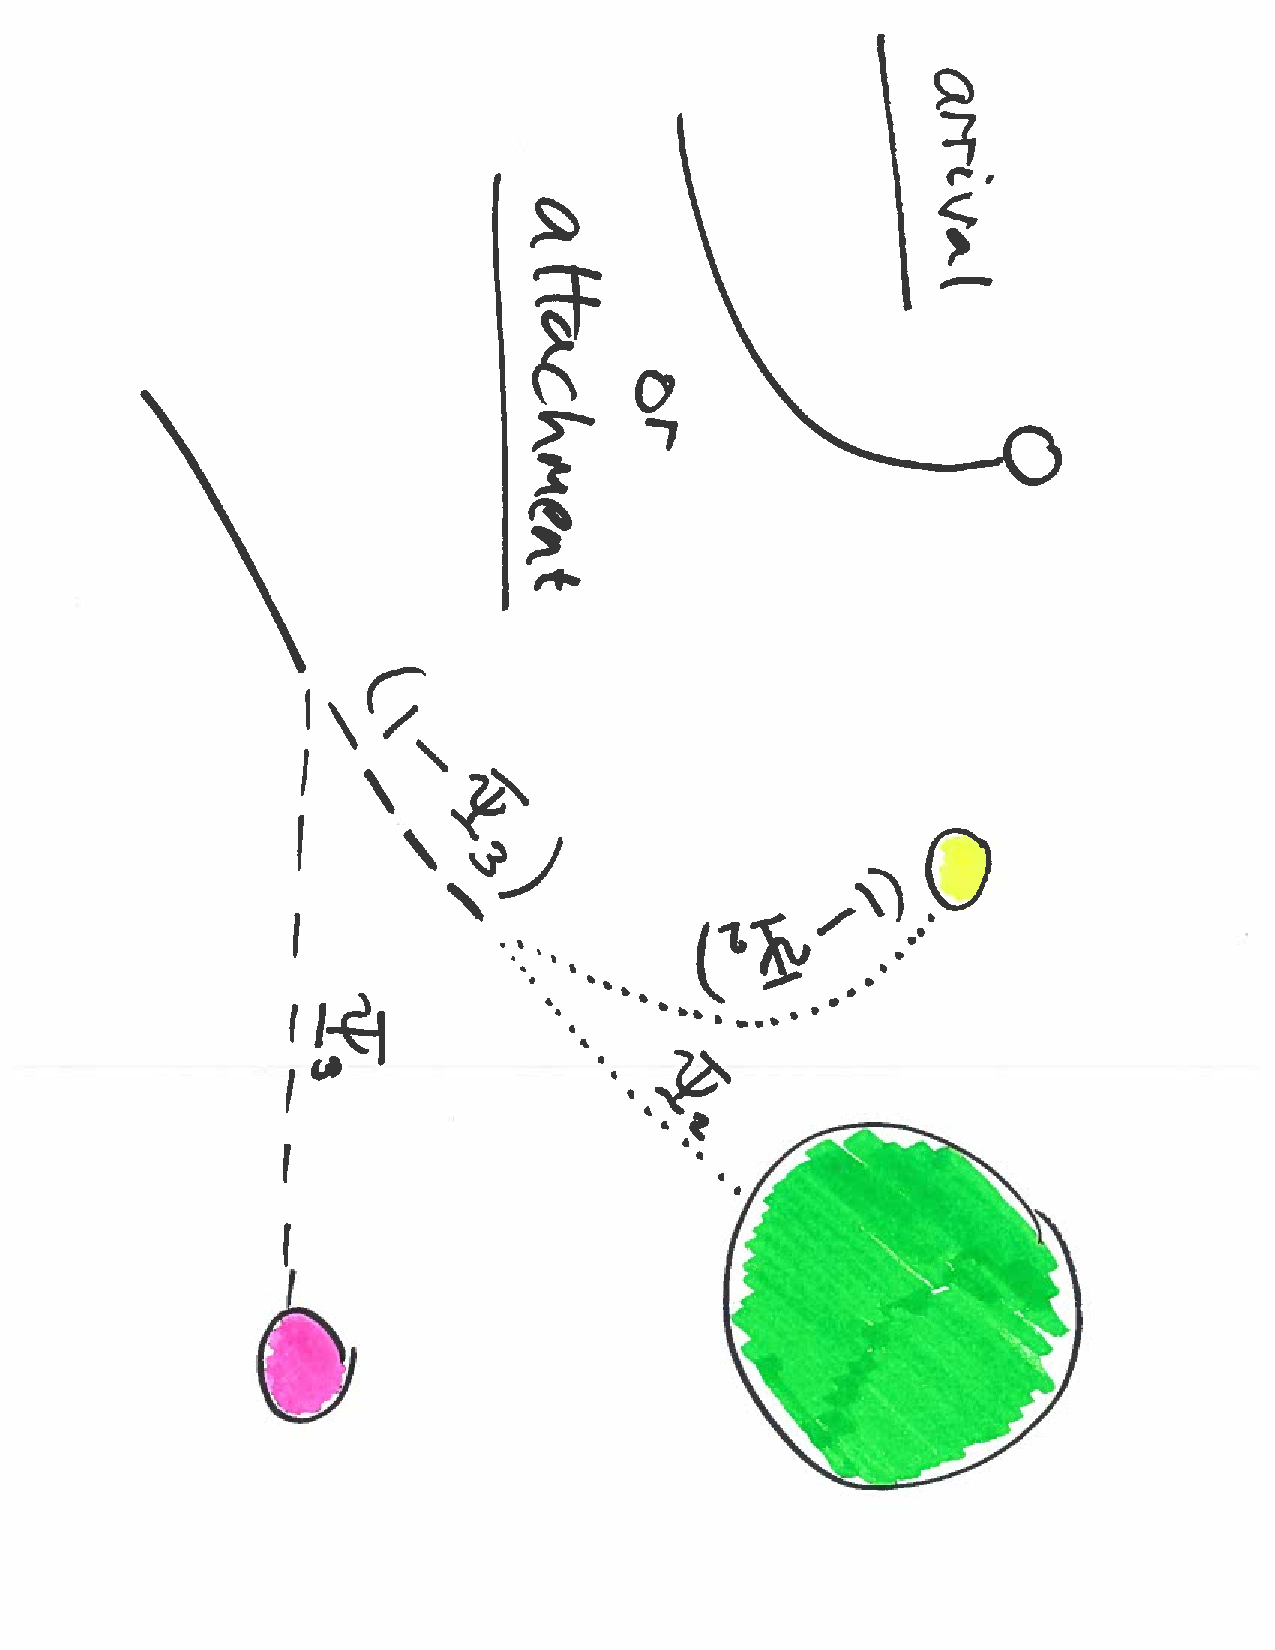
\includegraphics[angle=90,origin=c,scale=0.4]{fig/bntllatent2}
%\end{frame}

% \definecolor{darkgreenClj}{rgb}{0.25,.5,0.25}
% \definecolor{blueClj}{rgb}{0,0.33,0.66}
% \definecolor{redClj}{rgb}{0.66,0.0,0.0}
% \definecolor{purpleClj}{rgb}{0.33,0,0.66}
% \definecolor{cyanClj}{rgb}{0.0,0.5,0.5}
% \definecolor{orangeClj}{rgb}{0.75,0.35,0.0}
% \definecolor{grayClj}{rgb}{0.6,0.6,0.6}
% \definecolor{darkgrayClj}{rgb}{0.3,0.3,0.3}

\begin{frame}
	\frametitle{Sequence of paintboxes representation}
	% 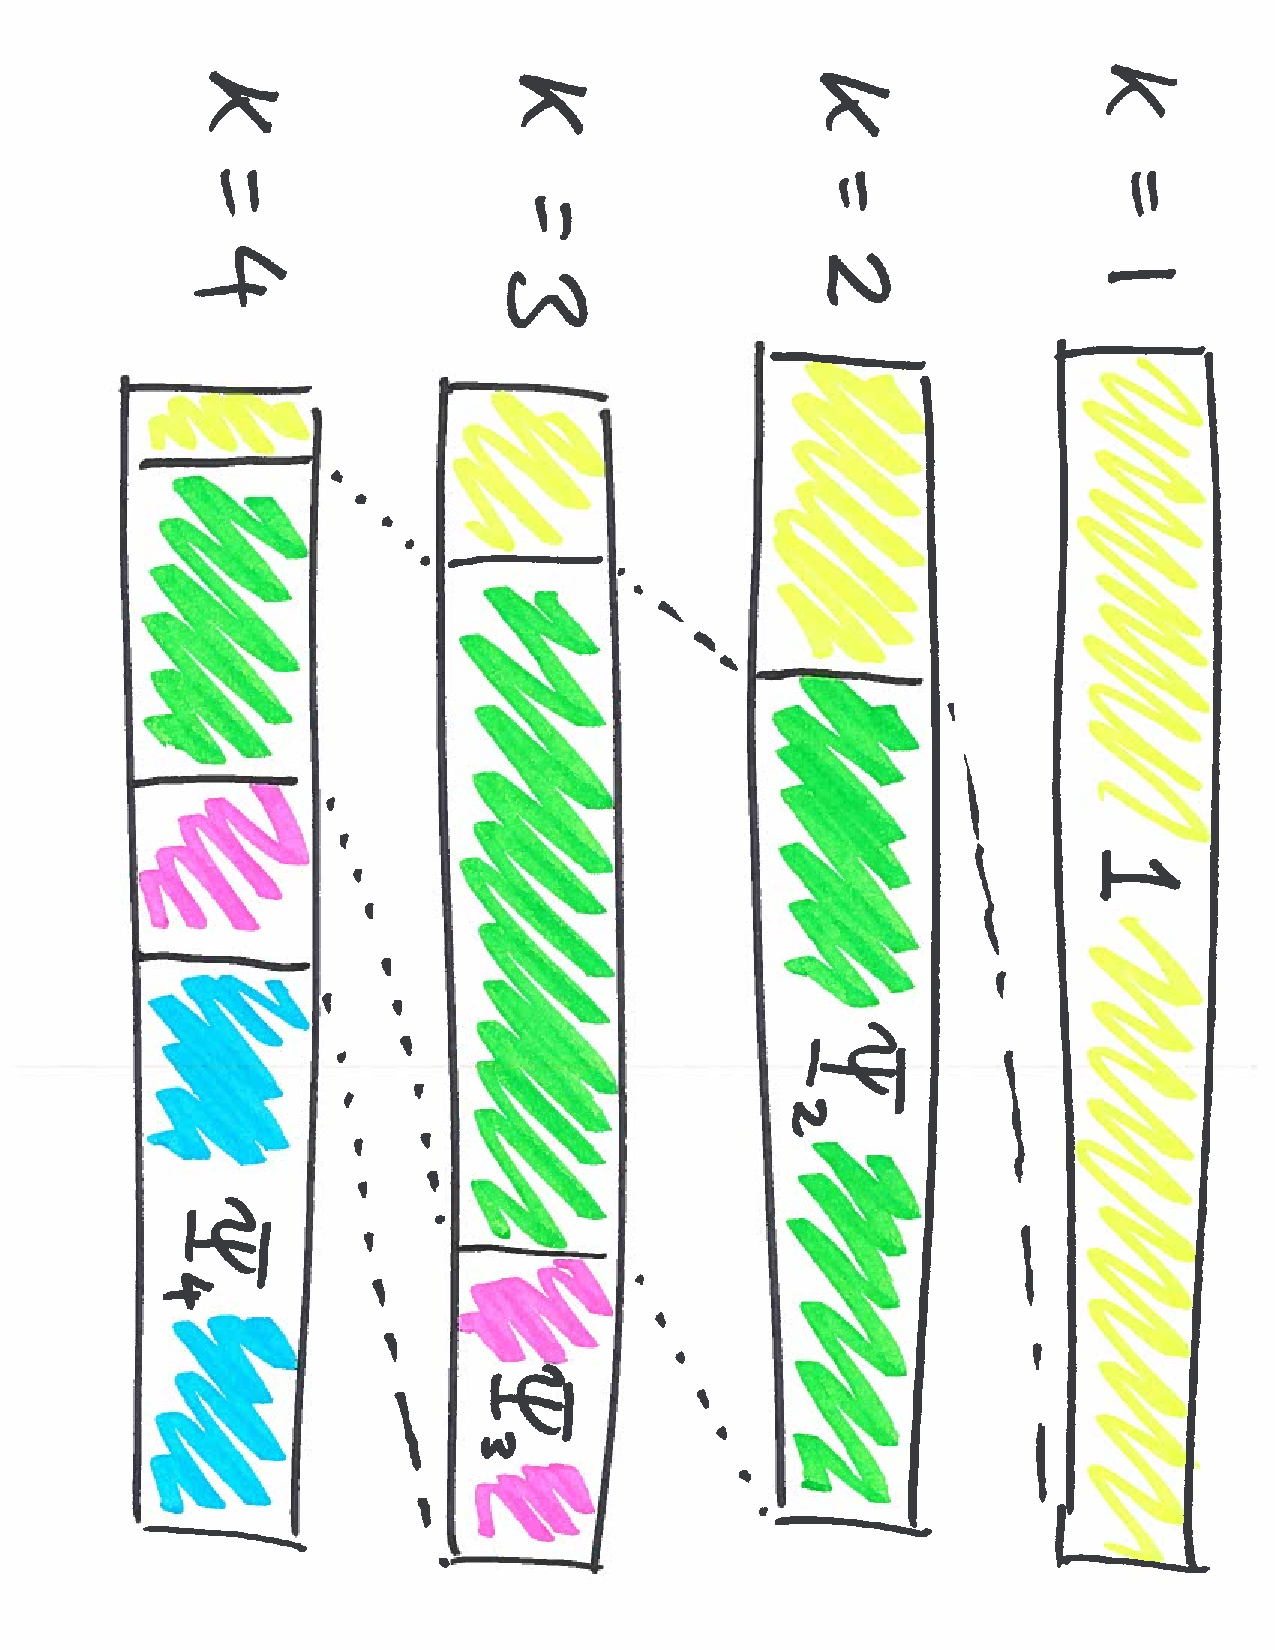
\includegraphics[angle=90,origin=c,scale=0.4]{fig/recursivescaling}
	% \vspace{-0.5cm}
	\begin{center}
	\makebox[\textwidth][c]{
	  \resizebox{0.95\textwidth}{!}{
	  	\begin{tikzpicture}

			% y offset for paintboxes
			\coordinate (pboff) at (0,-3);

			% draw paintboxes
			\def\psipic{{0.0,0.6,0.7}}%,0.9}} % these are (1-\psi_j)
			\def\blockcolors{{"0,0.33,0.66","0.75,0.35,0.0","0.25,.5,0.25"}}%,"0.6,0.6,0.6"}} % these are block colors
			\def\nrands{{3,3,6}}%,5}}
			\foreach \nouter in {0,...,2}{
				\draw ($(0,0)+\nouter*(pboff)$) -- ($(8,0)+\nouter*(pboff)$) -- ($(8,1)+\nouter*(pboff)$) -- ($(0,1)+\nouter*(pboff)$) -- cycle;
				\pgfmathparse{int(\nouter+1)};
				\let\nverts\pgfmathresult;
				\pgfmathparse{int(\nouter+2)};
				\let\nextnverts\pgfmathresult;
				\pgfmathparse{int(\nouter)};
				\let\prevnverts\pgfmathresult;
				\node at ($(-1.5,0.5)+\nouter*(pboff)$) {$T_{\nverts} < n < T_{\nextnverts}$};
				% \ifnum \nouter>0
				% 	\node at ($(10.0,1.0)+\nouter*(pboff)$) {$P_{j,\nverts}=P_{j,\prevnverts}(1-\Psi_{\nverts})$};
				% 	\node at ($(10.0,0.0)+\nouter*(pboff)$) {$P_{\nverts,\nverts}=\Psi_{\nverts}$};
				% \fi

				\edef\tmplower{1.0};
				\foreach \ninner in {0,...,\nouter}{
					% update color
					\pgfmathparse{\blockcolors[\nouter-\ninner]};
					\let\tmpcol\pgfmathresult;
					\definecolor{tmpcol}{rgb}{\tmpcol};
					% \node at ($(0.25*\nouter,-1*\ninner)$) [color=tmpcol] {\small \tmpcol};

					% update x coordinates
					\edef\tmpupper{\tmplower};
					\pgfmathparse{\psipic[\nouter-\ninner]*\tmplower};
					\global\let\tmplower\pgfmathresult;

					\pgfmathparse{int(\nouter-\ninner+1)};
					\let\tmpidx\pgfmathresult;
						% for testing
						% \node at ($(8*\tmpupper,0)+\nouter*(pboff)$) {u: \tmpupper, \ninner};
						% \node at ($(8*\tmplower,0)+\nouter*(pboff)$) {l: \tmplower, \ninner};
					% draw block
					\fill[color=tmpcol] ($(8*\tmplower,0)+\nouter*(pboff)$) rectangle ($(8*\tmpupper,1)+\nouter*(pboff)$);
					\node at ($(4*\tmplower+4*\tmpupper,0.5)+\nouter*(pboff)$) {$P_{\tmpidx,\nverts}$};
					\ifnum \ninner=\nouter
						\ifnum \nouter=0
							\node[anchor=south] at ($(4*\tmplower+4*\tmpupper,1)+\nouter*(pboff)$) {$P_{1,\nverts}=1$};
						\else
							\node[anchor=south] at ($(4*\tmplower+4*\tmpupper,1)+\nouter*(pboff)$) {$P_{1,\nverts}=P_{1,\prevnverts}(1-\Psi_{\nverts})$};
						\fi
					\fi

					\ifnum \ninner=0
						\ifnum \nouter>0
							\node[anchor=south] at ($(4*\tmplower+4*\tmpupper,1)+\nouter*(pboff)$) {$P_{\nverts,\nverts}=\Psi_{\nverts}$};
						\fi
					\fi
				}
				\pgfmathparse{\nrands[\nouter]};
				\let\numdots\pgfmathresult;
				\foreach \nunif [count=\i] in {1,...,\numdots}{
					\pgfmathparse{random()};
					\let\tmprnd\pgfmathresult;
					% \edef\tmprnd{rand}
					\fill[color=darkgrayClj] ($(8*\tmprnd,-0.3)+\nouter*(pboff)$) circle (2pt);% node[anchor=north,color=darkblue]{$U_{T_{\nverts}+\i}$};
					\draw[dashed,color=darkblue] ($(8*\tmprnd,-0.2)+\nouter*(pboff)$) -- ($(8*\tmprnd,1.0)+\nouter*(pboff)$);
				}
			}
	  	\end{tikzpicture}
	  }
	}
	\end{center}
\end{frame}


\section{Sampling and inference}
\begin{frame}
	\frametitle{Sampling and inference}
	Why a paper on sampling and inference for BNTL models?
	\pause
	\begin{itemize}
		\item Inference is notoriously difficult for \textit{non-exchangeable} structures
		\item Need to identify \textit{exchangeable substructures}
	\end{itemize}
\end{frame}

\begin{frame}
	\frametitle{Exchangeable substructure}
	\begin{center}
		\resizebox{\textwidth}{!}{\begin{tikzpicture}[>=stealth]%[transform canvas={xshift=-0.5cm}]
    % \node[font=\scriptsize] at (-8.5,0.5) {$t$} ;
    % row 1
    \draw[shift={(-8.0,0)}] (-4pt,0) node[anchor=east,font=\scriptsize] {$1$} -- (4pt,0) {};
    % \draw[dotted,shift={(-8.0,0.0)},color=gray] (0,0) -- (8.0,0) {};
    \draw[densely dashed] (-8.0,0.5) node[anchor=south,font=\scriptsize] {$T_1=1$} -- (-8.0,-3.5) ;
    \foreach \x/\xtext/\xco in {0.0//red, 0.1//red, 0.2//red, 0.3//red, 0.6//red, 0.9//red, 1.3//red, 1.5//red, 1.7//red, 1.9//red, 2.2//red}
    	\fill[color=\xco] (-8.0+3*\x,0) circle (2pt) node[anchor=south,font=\scriptsize,color=black] {$\xtext$};
    \draw[densely dotted,color=red] (0.1,0.25) -- (-8.1,0.25) -- (-8.1,-0.25) -- (0.1,-0.25) ;
    % row 2
    \draw[shift={(-8.0,-1.0)}] (-4pt,0) node[anchor=east,font=\scriptsize] {$2$} -- (4pt,0) {};
    % \draw[dotted,shift={(-8.0,-1.0)},color=gray] (0,0) -- (8.0,0) {};
    \draw[densely dashed] (-8.0+1.2,0.5) node[anchor=south,font=\scriptsize] {$T_2$} -- (-8.0+1.2,-3.5) ;
    \foreach \x/\xtext/\xco in {0.4//blue, 0.5//blue, 0.7//blue, 0.8//blue, 1.1//blue, 1.4//blue, 1.8//blue, 2.1//blue, 2.4//blue}
    	\fill[color=\xco] (-8.0+3*\x,-1.0) circle (2pt) node[anchor=south,font=\scriptsize,color=black] {$\xtext$};
    \draw[densely dotted,color=blue] (-8.1+1.4,0.25) -- (-8.1+1.4,-1.25) -- (0.1,-1.25) ;
    % row 3
    \draw[shift={(-8.0,-2.0)}] (-4pt,0) node[anchor=east,font=\scriptsize] {$3$} -- (4pt,0) {};
    % \draw[dotted,shift={(-8.0,-2.0)},color=gray] (0,0) -- (8.0,0) {};
    \draw[densely dashed] (-8.0+3.0,0.5) node[anchor=south,font=\scriptsize] {$T_3$} -- (-8.0+3.0,-3.5) ;
    \foreach \x/\xtext/\xco in {1.0//green, 1.2//green, 2.3//green}
    	\fill[color=\xco] (-8.0+3*\x,-2.0) circle (2pt) node[anchor=south,font=\scriptsize,color=black] {$\xtext$};
    \draw[densely dotted,color=green] (-8.1+3.2,0.25) -- (-8.1+3.2,-2.25) -- (0.1,-2.25) ;
    % row 4
    \draw[shift={(-8.0,-3.0)}] (-4pt,0) node[anchor=east,font=\scriptsize] {$4$} -- (4pt,0) {};
    % \draw[dotted,shift={(-8.0,-3.0)},color=gray] (0,0) -- (8.0,0) {};
    \draw[densely dashed] (-8.0+4.8,0.5) node[anchor=south,font=\scriptsize] {$T_4$} -- (-8.0+4.8,-3.5) ;
    \foreach \x/\xtext/\xco in {1.6//magenta, 2.0//magenta}%, 2.4//magenta}
    	\fill[color=\xco] (-8.0+3*\x,-3.0) circle (2pt) node[anchor=south,font=\scriptsize,color=black] {$\xtext$};
    \draw[densely dotted,color=magenta] (-8.1+5.0,0.25) -- (-8.1+5.0,-3.25) -- (0.1,-3.25) ;
\end{tikzpicture}}
	\end{center}
\end{frame}

\begin{frame}
	\frametitle{Gibbs structure}
	The joint probability has \textbf{Gibbs structure} due to left-neutrality
	\begin{equation*}
	P(\text{graph}|\bfT) = \prod_{j=1}^K P(\text{choose }j\ d_j-1\text{ times out of } n - T_j \text{ trials })
	\end{equation*}
	\begin{itemize}
		\item $K$ = \#vertices
		\item $n$ = \#edges
		\item $d_j$ = degree of vertex $j$
		\item $T_j$ = arrival time of vertex $j$
	\end{itemize}
\end{frame}

\begin{frame}
	\frametitle{Gibbs structure}
	Explicitly,
	\begin{equation*}
	p(\text{graph}|\bfT) = \frac{\Gamma(d_1 - \alpha)}{\Gamma(n - K\alpha)}\prod_{j=2}^K \frac{\Gamma(T_j - j\alpha)\Gamma(d_j - \alpha)}{\Gamma(T_j - 1 - (j-1)\alpha)\Gamma(1-\alpha)}
	\end{equation*}
	\begin{itemize}
		\item $K$ = \#vertices
		\item $n$ = \#edges
		\item $d_j$ = degree of vertex $j$
		\item $T_j$ = arrival time of vertex $j$
	\end{itemize}
\end{frame}

\begin{frame}
	\frametitle{Available data}
	\begin{center}
		\begin{tabular}{ll}
			\textbf{Observation} & \textbf{Unobserved variables} \\
			\hline
			Entire history & $\alpha,\phi,\bfPsi$ \\
			Degrees in arrival order & $\alpha,\phi,\bfPsi, \bfT$ \\
			Snapshot & $\alpha,\phi,\bfPsi,\bfT,\sigma$
		\end{tabular}
	\end{center}
	\begin{itemize}
		\item $\alpha$ = BTNL parameter $\in (-\infty, 1)$
		\item $\phi$ = arrival distribution parameters
		\item $\bfPsi$ = latent sociabilities
		\item $\bfT$ = arrival times
		\item $\sigma$ = arrival order
	\end{itemize}
\end{frame}

\begin{frame}
	\frametitle{Gibbs sampler}
	\begin{center}
		\begin{tabular}{l|l}
			\textbf{Variable} & \textbf{Gibbs sampling scheme} \\
			\Xhline{4\arrayrulewidth}
			\rule{0pt}{3ex}
			$\alpha$ & MCMC, e.g. slice sampling \\
			\hline
			\rule{0pt}{3ex}
			$\phi$ & Depends on arrival dist. family $\Lambda_\phi$ \\
			\hline
			\rule{0pt}{3ex}
			$\mathbf{\Psi}$ & $\Psi_j | \text{graph}, \mathbf{\Psi}_{\setminus j} \sim \text{Beta}(d_{j} - \alpha, \bar{d}_{j-1} - (j-1)\alpha)$ \\
			& \quad where $\bar{d}_{j} = \sum_{i=1}^j d_{j}$ \\
			& \quad can marginalise out $\bfPsi$ \\
			\hline
			\rule{0pt}{3ex}
			$\mathbf{T}$ & Simple update for $T_j$, can't move past neighbours \\
			\hline
			\rule{0pt}{3ex}
			$\sigma$ & Initialise in descending degree order \\
			& \quad use M-H with adjacent swap proposal $\sigma_j \leftrightarrow \sigma_{j+1}$\\
			& \quad fast to compute due to Gibbs structure
		\end{tabular}
	\end{center}
\end{frame}

%\begin{frame}
%	\frametitle{Sampling $\bfPsi$}
%	Beta prior on $\Psi_j$, plus Gibbs structure, give
%	\begin{equation*}
%	\Psi_j \mid \text{graph}, \bfPsi_{\setminus j} \sim \text{Beta}(d_{j} - \alpha, \bar{d}_{j-1} - (j-1)\alpha) \;,
%	\end{equation*}
%	\small{where $\bar{d}_j = \sum_{i=1}^j d_i$}
%\end{frame}
%
%\begin{frame}
%	\frametitle{Sampling $\alpha,\phi$}
%	\begin{itemize}
%		\item One-dimensional unnormalized density for $\alpha$
%		\item For $\phi$ depends on arrival distribution family
%	\end{itemize}
%
%\end{frame}
%
%\begin{frame}
%	\frametitle{Sampling $\bfT$}
%	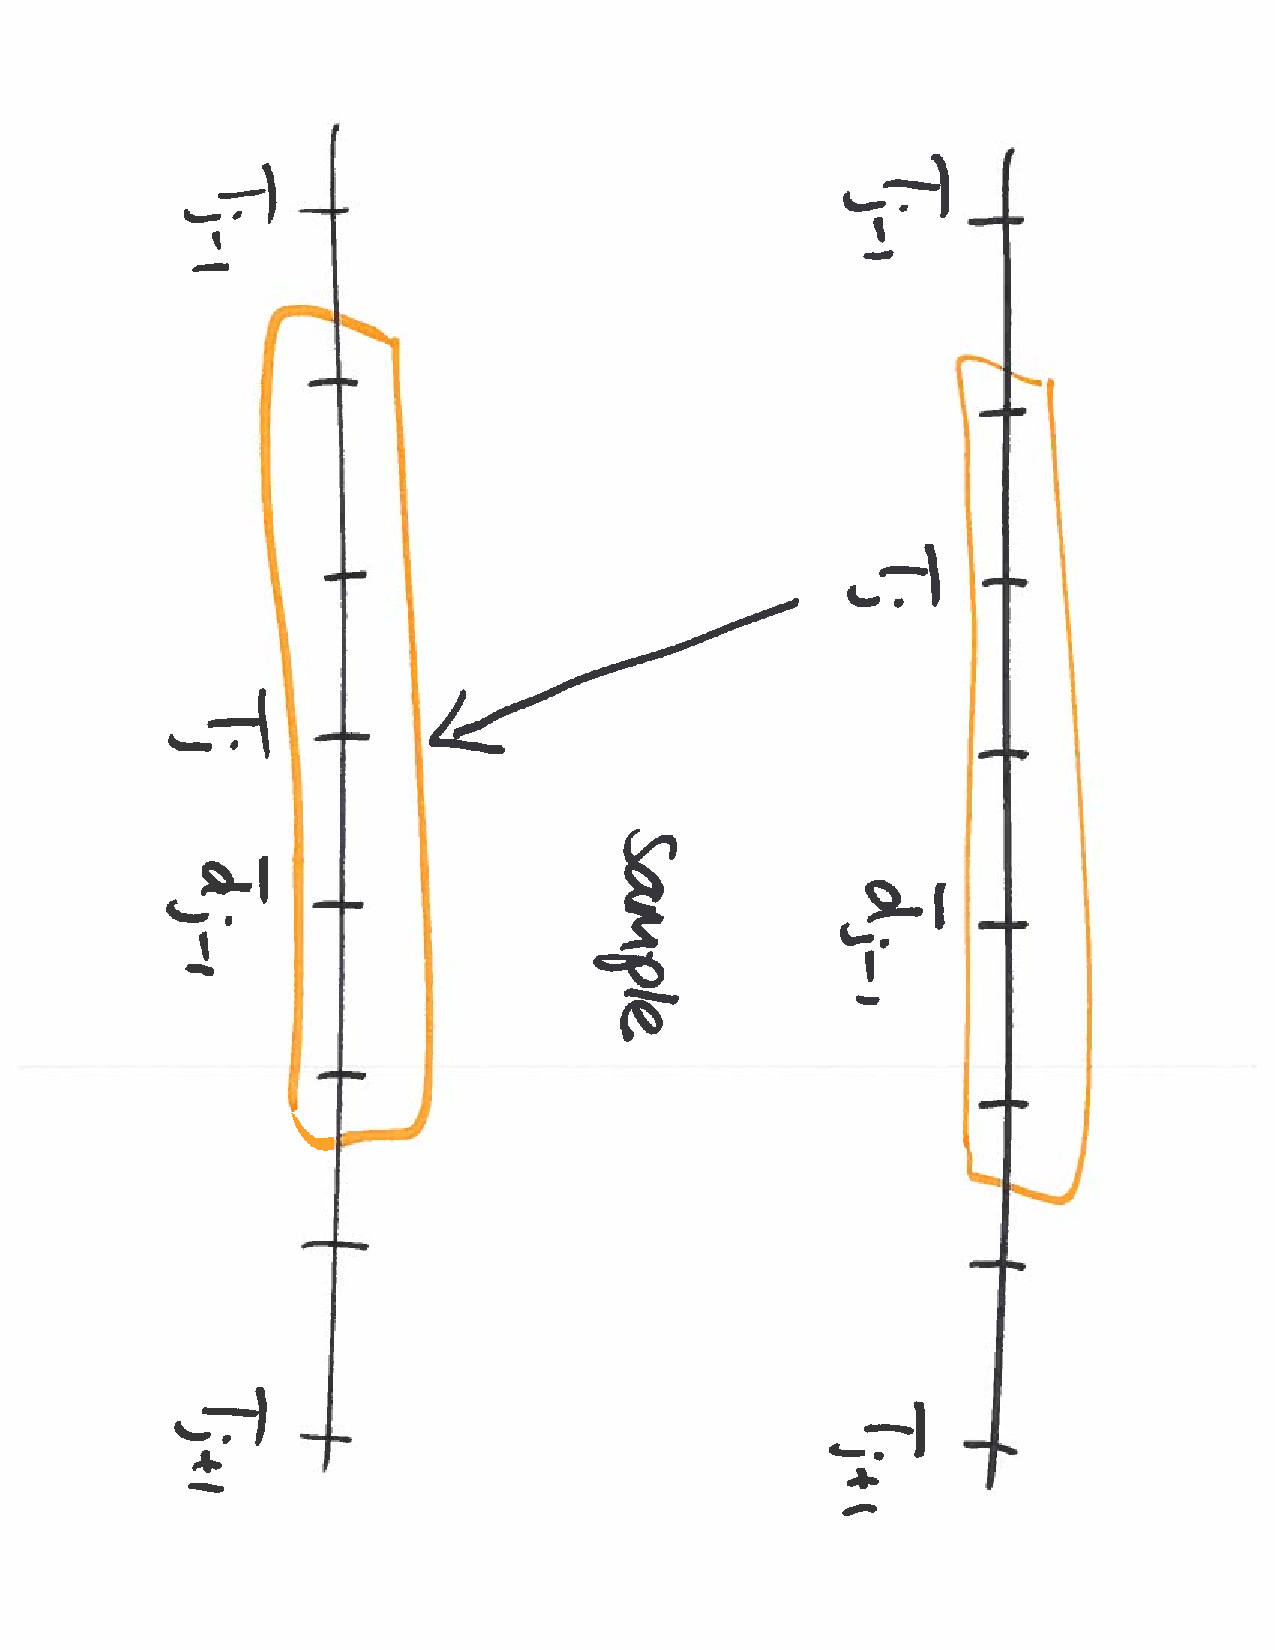
\includegraphics[angle=90,origin=c,scale=0.4]{fig/tsampling}
%\end{frame}
%
%\begin{frame}
%	\frametitle{Sampling $\sigma$}\
%
%	\begin{itemize} 
%	\item Initialise in descending degree order
%	\item Use Metropolis-Hastings with adjacent swap proposal $\sigma_j \leftrightarrow \sigma_{j+1}$
%	\end{itemize}
%\end{frame}

\begin{frame}
	\frametitle{Point estimation}
	If entire history observed,\textbf{maximum a posterior} (or \textbf{maximum likelihood}) estimates for $\alpha, \phi$ computable
\end{frame}

\section{Experiments}
\begin{frame}
	\frametitle{Experiments}
	\begin{itemize}
		\item Gibbs: parameter recovery
		\item Gibbs: scalability
		\item Point estimation with massive graphs
	\end{itemize}
\end{frame}

\begin{frame}
	\frametitle{Parameter recovery}
	\begin{itemize}
		\item Simulate 500 edges with fixed $\alpha$ 
		\item Arrivals either $\PYP$ or $\Geom$
		\item Observe final snapshot of the graph
	\end{itemize}
	\begin{table}[h]
		%  \caption{Results of Gibbs sampling experiments on synthetic data $(\alpha^* = 0.75)$. The top four rows show results from each of four different BNTL models fit to a synthetic graph with 500 edges generated by the coupled $\PYP$ BNTL model; the bottom four rows show the same BNTL models fit to a synthetic graph with $\Geom(0.25)$-distributed interarrivals.}
		\label{tab:ess}
		\vspace*{-0.75\baselineskip}
		\begin{center}
			\resizebox{1.0\textwidth}{!}{
				\begin{tabular}{lllll}
					Gen. arrival distn. & Inference model & $|\hat{\alpha} - \alpha^*|$ & Pred. log-lik.  \\
					\hline
					$\PYP(1.0,0.75)$ &  $(\tau,\PYP(\theta,\tau))$ &  \textbf{0.046 $\pm$ 0.002}   & -\textbf{2637.0 $\pm$ 0.1}  \\ 
					
					$\PYP(1.0,0.75)$  &  $(\alpha,\Geom(\beta))$  &  {0.049 $\pm$ 0.004} & -2660.5 $\pm$ 0.7  \\ 
					\hline
					
					$\Geom(0.25)$ & $(\tau,\PYP(\theta,\tau))$ &  0.086 $\pm$ 0.002   & -2386.8 $\pm$ 0.1  \\  
					
					$\Geom(0.25)$ & $(\alpha,\Geom(\beta))$ &  \textbf{0.043 $\pm$ 0.003}  & -\textbf{2382.6 $\pm$ 0.2}  \\ 
					
					\end{tabular}
					}
				\end{center}
			\end{table}
			
% where $\mathbf{S} := \frac{1}{K_n - 1} \sum_{j>1} (\bar{d}_{j-1} - T_j)$
\end{frame}

\begin{frame}
	\frametitle{Scalability}
	\begin{itemize}
		\item Simulate with fixed $\alpha$ and $\Geom(\beta)$ arrivals
	\end{itemize}
	
	\begin{table}[t]
		\label{tab:ess:scale:n}
		\vspace*{-0.25\baselineskip}
		\begin{center}
			%  \resizebox{0.6\textwidth}{!}{
			\begin{tabular}{l  ll}
				& $100$ edges &  $10000$ edges \\ 
				\hline
				$|\hat{\alpha} - \alpha^*|$ & 0.12 $\pm$ 0.01 &  0.01 $\pm$ 0.00 \\ 
				
				$|\hat{\beta} - \beta^*|$ &  0.02 $\pm$ 0.00  &    0.00 $\pm$ 0.00  \\ 
				
				Effective Sample Size &  0.90 $\pm$ 0.04  &   0.75 $\pm$ 0.08  \\  
				
				Runtime (s) &  21 $\pm$ 0   &  2267 $\pm$ 2  \\ 
				
			\end{tabular}
			%}
		\end{center}
	\end{table}
	\begin{itemize}
		\item Runtime linear in \#edges
		\item Most expensive Gibbs update is for $\bfT$
	\end{itemize}
\end{frame}

\begin{frame}
	\frametitle{MLEs for SNAP datasets}
	\begin{itemize}
		\item SNAP datasets
		\item Fit point estimates for $\alpha, \phi$
		\item Fit: coupled $\PYP$, uncoupled $\PYP$ and $\Geom(\beta)$ arrivals
	\end{itemize}
\end{frame}

\begin{frame}
	\frametitle{MLEs for SNAP datasets}
	Ask Ubuntu
	\begin{itemize}
		\item Estimates of $\PYP$ parameters vary significantly between coupled and uncoupled
		\begin{itemize}
			\item $\hat{\theta}, \hat{\alpha} = 18080, 0.25$
			\item $\hat{\theta}, \hat{\alpha}, \hat{\tau} = -0.99, -2.54, 0.99$
		\end{itemize}
		\item Edge exchangeable models misspecified ($\eta > 2$)
		\item Using $\Geom$ estimates $\eta$ well
	\end{itemize}
\end{frame}
	
%\begin{frame}
%	\frametitle{MLEs for SNAP datasets}
%	Though not for all datasets
%	\begin{table}[!ht]
%		\begin{center}
%			\color{lightgray}{
%				\resizebox{1.05\textwidth}{!}{
%					\begin{tabular}{llll | lllllll}
%						\multirow{2}{*}{Dataset} & \multicolumn{3}{c}{Coupled $\PYP(\theta,\alpha)$}  & &  \multicolumn{2}{c}{Uncoupled $\PYP(\theta,\tau)$} &  & \multicolumn{3}{c}{$\Geom(\geom)$}                             \\
%						\cline{2-4} \cline{6-7} \cline{9-11}
%						& $(\hat{\theta},\hat{\alpha})$ & $\hat{\eta}$           & Pred. l-l.            & $\hat{\alpha}$    & $(\hat{\theta},\hat{\tau})$ & Pred. l-l.     &     & $\hat{\beta}$  & $\hat{\eta}$   & Pred. l-l.                             \\
%						\hline
%						Ask Ubuntu  & (18080, 0.25) & 1.25   & -3.707e6              & -2.54            & (-0.99, 0.99)    & -3.678e6  &   &  0.083 & 2.32    & \textbf{-3.678e6}                         \\
%						UCI social network & (320.4, 4.4e-11) & --   & -1.600e5            & -4.98             & (5.50, 0.52)     & \textbf{-1.595e6}   &  & 0.016  & 2.10  & -1.596e5                    \\
%						EU email   & (113.6, 2.5e-14)  & --    & \textbf{-8.06e5}              & -1.86              & (113.6, 9.2e-10)      & \textbf{-8.06e5}  &   & 0.001  & 2.00   & -8.07e5                     \\
%						Math Overflow & (2575, 0.15) & 1.15  & -1.685e6              & -6.62           & (-0.97, 0.997)    & -1.670e6 &    & 0.025  & 2.19   & \textbf{-1.670e6}                \\
%						Stack Overflow & (297600, 0.11) & 1.11 & -3.358e8             & -8.94            & (-1.0, 1.0)      &  -3.333e8  &    &  0.020  & 2.21   & \textbf{-3.333e8}                 \\
%						Super User  & (20640, 0.24) & 1.24  & -5.855e6            & -4.19          & (-0.996, 1.0)      &  \textbf{-5.775e6}   &  & 0.067 & 2.37    & -5.775e6              \\
%						Wikipedia talk pages  & (14870, 0.54) & 1.54  & -3.074e7          & -0.25            & (-1.0, 1.0)   & \textbf{-3.066e7}  &   & 0.073  & 2.10   & -3.066e7                   
%					\end{tabular}
%				}}
%			\end{center}
%			\vspace*{-\baselineskip}
%		\end{table}
%	\end{frame}

\begin{frame}
	\frametitle{Conclusion}
	\begin{itemize}
		\item BNTL models are \textit{flexible}
		\item BNTL models are \textit{tractable}
	\end{itemize}
\end{frame}

\begin{frame}
	\frametitle{References}
	\tiny{\bibliographystyle{unsrt}
	\bibliography{refs}}
\end{frame}

\end{document}
